%\documentclass[a4papper, 12pt, titlepage]{book}
\documentclass[a4papper, 12pt, parskip, headsepline]{book}

\usepackage[utf8]{inputenc}
\usepackage[T1]{fontenc}
\usepackage[normalem]{ulem}
\usepackage[francais,english]{babel}% langue principale = english
\usepackage{graphicx}
\usepackage[labelfont=bf]{caption}
\usepackage{subcaption}
%\usepackage{a4wide}
\usepackage{ulem}
\usepackage{enumerate}
\usepackage{array}
\usepackage{amsmath}
\usepackage{amssymb}
\usepackage{mathrsfs}
\usepackage{esvect}
\usepackage{textcomp}
\usepackage{mathtools}
\usepackage{verbatim}
\usepackage{listings}
\usepackage{url}
\usepackage{moreverb}
\usepackage{placeins} 
%\usepackage[table]{xcolor}
\usepackage{array,multirow,makecell}
\usepackage{lettrine}
\usepackage{oldgerm}
\usepackage{import}
\usepackage{hyperref}
%\usepackage[Bjornstrup]{fncychap}
\usepackage{tabulary}
\usepackage{pdfpages}
\newcolumntype{K}[1]{>{\centering\arraybackslash}p{#1}}

%\usepackage{titlesec}
%\makeatletter
%\@addtoreset{chapter}{part}
%\makeatother
%\titleformat{\part}[display]
%{\normalfont\LARGE\bfseries\centering}{}{0pt}{}

\usepackage[tight]{shorttoc}
\usepackage{todonotes}
\usepackage{minitoc}
\usepackage{helvet}
\usepackage{mathabx} % For degrees
\usepackage{float}
\usepackage{rotating} % To rotate huge tables
\usepackage{feynmp}
%\usepackage{feynman}
\usepackage{ifpdf}
\ifpdf
  \DeclareGraphicsRule{*}{mps}{*}{}
\fi
%\usepackage{fancyhdr}
%\pagestyle{fancy}
%%\fancyhead{}
%%\fancyhead[RO,LE]{\thsection}
%%\fancyfoot{}
%%\fancyfoot[LE,RO]{\thepage}
%%\fancyfoot[LO,CE]{Chapter \thechapter}
%%\fancyfoot[CO,RE]{Author Name}
%\fancyhead[LE,RO]{\slshape \rightmark}
%\fancyhead[LO,RE]{\slshape \leftmark}
%\fancyfoot[C]{\thepage}
\renewcommand{\chaptermark}[1]{%
 \markboth{\MakeUppercase{%
 \chaptername}\ \thechapter:%
 \ #1}{}}

\hypersetup{
  backref=true, %permet d'ajouter des liens dans... pagebackref=true,%...les bibliographies
  hyperindex=true, %ajoute des liens dans les index.
  colorlinks=true, %colorise les liens
  breaklinks=true, %permet le retour à la ligne dans les liens trop longs urlcolor= blue, %couleur des hyperliens
  linkcolor= blue, %couleur des liens internes
  bookmarks=true, %créé des signets pour Acrobat
  bookmarksopen=true,
  pdftitle={Intelligent detection layers for tracking in high energy physics}, 
  pdfauthor={Benjamin BOITRELLE},
  pdfsubject={Mac OS X}
}

\newcommand{\sommaire}{\shorttoc{Sommaire}{1}}

% \usepackage{fullpage}

%\usepackage[style=long,nonumberlist,toc,xindy,acronym,nomain]{glossaries}

%\usepackage{geometry}
%\geometry{hmargin=2.5cm}

 \definecolor{light-gray}{gray}{0.85}
 %\newcolumntype{M}[1]{>{\raggedright}m{#1}}
 \newcolumntype{M}[1]{>{\centering\arraybackslash}m{#1}} % To center text in table
 
\renewcommand{\baselinestretch}{0.9}
%\newcommand{\noyau}[3]{\prescript{#2}{#3}{\mathrm{#1}}}

\lstset{language=c++,numbers=left,tabsize=2,breaklines=true}

\makeatletter
\def\clap#1{\hbox to 0pt{\hss #1\hss}}%
\def\ligne#1{%
    \hbox to \hsize{%
\vbox{\centering #1}}}%
\def\haut#1#2#3{%
    \hbox to \hsize{%
        \rlap{\vtop{\raggedright #1}}%
        \hss
        \clap{\vtop{\centering #2}}%
        \hss
\llap{\vtop{\raggedleft #3}}}}%
\def\bas#1#2#3{%
    \hbox to \hsize{%
        \rlap{\vbox{\raggedright #1}}%
        \hss
        \clap{\vbox{\centering #2}}%
        \hss
\llap{\vbox{\raggedleft #3}}}}%
\def\maketitle{%
    \thispagestyle{empty}\vbox to \vsize{%
        \haut{}{\@blurb}{}
        \vfill
        \vspace{3cm}
        \begin{center}
            \usefont{OT1}{ptm}{m}{n}
            \huge \@title
        \end{center}
        \par
        \hrule height 4pt
        \par
        \begin{flushright}
            \usefont{OT1}{phv}{m}{n}
            \Large \@author
            \par
        \end{flushright}
        \vspace{1cm}
        \vfill
        \vfill
        \bas{}{\@location, \@date}{}
        \vspace{1cm}
        %\includegraphics[scale = 0.1]{Logos/LogoUCBL}
        %\hfill
        %\includegraphics[scale = 0.2]{Logos/logo_IPHC_10cm}
        %\hfill
        %\includegraphics[scale = 0.15]{Logos/CNRS_logo}
        %\hfill
    }%
    \cleardoublepage
}
\def\date#1{\def\@date{#1}}
\def\author#1{\def\@author{#1}}
\def\title#1{\def\@title{#1}}
\def\location#1{\def\@location{#1}}
\def\blurb#1{\def\@blurb{#1}}
\date{}
\author{}
\title{}
\location{DESY - Hamburg}\blurb{}
\makeatother
\title{Intelligent detection layers for tracking in high energy physics}
\author{Benjamin \textsc{Boitrelle}}

\location{DESY - Hamburg}
%\blurb{%
%    Université de Strasbourg\\
%    École Doctorale de Physique et Chimie-Physique (ED182) \\ 
%    \textbf{Thèse}\\[1em]
%Directeur de thèse : Jérôme \textsc{Baudot}\\ % 
%Co-directeur de thèse : Ingrid \textsc{Maria Gregor}\\ }% 

\usepackage[nottoc, notlof, notlot]{tocbibind}
\usepackage[toc,acronym,nomain,indexonlyfirst]{glossaries}
\makeglossaries
\setacronymstyle{long-short}
\renewcommand*{\glslinkcheckfirsthyperhook}{% To make a reference only for the first glossary entry
  \ifglsused{\glslabel}%
  {%
    \setkeys{glslink}{hyper=false}%
  }%
  {}%
}
\renewcommand*{\glstextformat}[1]{\textcolor{black}{#1}} % To make glossary black and not blue

\newcommand*{\glswriteentry}[2]{%  
  \ifglsindexonlyfirst  
    \ifglsused{#1}{}{#2}%  
  \else  
    #2%  
  \fi  
}
\setlength{\parskip}{1ex plus 0.5ex minus 0.2ex}

\newenvironment{dedication}
  {\clearpage           % we want a new page
   \thispagestyle{empty}% no header and footer
   \vspace*{\stretch{1}}% some space at the top 
   \itshape             % the text is in italics
   \raggedleft          % flush to the right margin
  }
  {\par % end the paragraph
   \vspace{\stretch{3}} % space at bottom is three times that at the top
   \clearpage           % finish off the page
  }


% Better page layout for A4 paper, see memoir manual.
%\settrimmedsize{297mm}{210mm}{*}
%\setlength{\trimtop}{0pt} 
%\setlength{\trimedge}{\stockwidth} 
%\addtolength{\trimedge}{-\paperwidth} 
%\settypeblocksize{634pt}{448.13pt}{*} 
%\setulmargins{4cm}{*}{*} 
%\setlrmargins{*}{*}{1.5} 
%\setmarginnotes{17pt}{51pt}{\onelineskip} 
%\setheadfoot{\onelineskip}{2\onelineskip} 
%\setheaderspaces{*}{2\onelineskip}{*} 
%\checkandfixthelayout

\begin{document}
    
  \frontmatter
    \includepdf[pages=-]{coverThesis}
    %\maketitle
    \input{aknowledgements.tex}
    %\setcounter{page}{1}

    \dominitoc
    \tableofcontents
    \listoffigures
    \listoftables
    %\listoftodos
%	\sommaire

%----------------------------------------------------------------------------------------
%	DEDICATION
%----------------------------------------------------------------------------------------

%\begin{dedication}
%  À ma famille, mes amis, Frédéric Courant et Jamy Gourmaud.
%\end{dedication}
    
    \newacronym{SM}{SM}{Standard Model}
\newacronym{EM}{EM}{electromagnetic interaction}
\newacronym{QED}{QED}{Quantum Electrodynamic}
\newacronym{QCD}{QCD}{Quantum Chromodynamics}
\newacronym{QFT}{QFT}{Quantum Field Theory}
\newacronym{LHC}{LHC}{Large Hadron Collider}
\newacronym{LEP}{LEP}{Large Electron Positron collider}
\newacronym{ILD}{ILD}{International Large Detector}
\newacronym{SiD}{SiD}{Silicon Detector}
\newacronym{PFA}{PFA}{Particle Flow Algorithm}
\newacronym{TPC}{TPC}{Time-Projection-Chamber}
\newacronym{ILC}{ILC}{International Linear Collider}
\newacronym{CLIC}{CLIC}{Compact LInear Collider}
\newacronym{SRF}{SRF}{Superconducting Radio-Frequency}
\newacronym{DC}{DC}{Direct-current}
\newacronym{BDS}{BDS}{Beam Delivery System}
\newacronym{RTML}{RTML}{Ring To the Main Linac}
\newacronym{IR}{IR}{interaction region}
\newacronym{IP}{IP}{interaction point}
\newacronym{VXD}{VXD}{Vertex Detector}
\newacronym{SIT}{SIT}{Silicon Internal Tracker}
\newacronym{SET}{SET}{Silicon External Tracking}
\newacronym{ETD}{ETD}{End-cap Tracking Detector}
\newacronym{FTD}{FTD}{Forward Tracking Detector}
\newacronym{ECAL}{ECAL}{Electromagnetic CALorimeter}
\newacronym{HCAL}{HCAL}{HAdronic CALanalogue HCALorimeter}
\newacronym{AHCAL}{AHCAL}{Analogue HCAL}
\newacronym{SDHCAL}{SDHCAL}{Semi-Digital HCAL}
\newacronym{GRPC}{GRPC}{Glass Resistive Plate Chamber}
\newacronym{LHCAL}{LHCAL}{Low angle Hadron CALorimeter}
\newacronym{PLUME}{PLUME}{Pixelated Ladder with Ultra-low Material Embedding}
\newacronym{CMOS}{CMOS}{Complementary Metal Oxide Semi-conductor}
\newacronym{FPCCD}{FPCCD}{Fine Pixels Charged Coupled-Device}
\newacronym{CCD}{CCD}{Charged Coupled-Device}
\newacronym{ASIC}{ASIC}{Application-Specified Integrated Circuit}
\newacronym{DEPFET}{DEPFET}{Depleted P- Channel Field Effect Transistor}
\newacronym{MIMOSA}{MIMOSA}{Minimum Ionizing MOS Active pixel sensor}
\newacronym{APS}{APS}{Active Pixel Sensor}
\newacronym{MAPS}{MAPS}{Monolithic Active Pixel Sensor}
\newacronym{MIP}{MIP}{Minimum Ionizing Particle}
\newacronym{DAQ}{DAQ}{Data AcQuisition}
\newacronym{FPN}{FPN}{Fixed Pattern Noise}
\newacronym{TN}{TN}{Temporal Noise}
\newacronym{SiC}{SiC}{Silicon Carbide}
\newacronym{OKF}{OKF}{Optiprint-Kapton-Flex-cable}
\newacronym{JTAG}{JTAG}{Joint Test Action Group}
\newacronym{ZIF}{ZIF}{Zero Insertion Force}
\newacronym{SUZE}{SUZE}{Suppression de zéro}
\newacronym{CDS}{CDS}{Correlated Double Sampling}
\newacronym{SNR}{SNR}{Signal to Noise ratio}
\newacronym{TAF}{TAF}{TAPI Analysis Framework}
\newacronym{LCIO}{LCIO}{Linear Collider I/O}
\newacronym{Marlin}{Marlin}{Modular Analysis and Reconstruction for the LINear collider}
\newacronym{GEAR}{GEAR}{GEometry Api for Reconstruction}
\newacronym{ISR}{ISR}{Initial State Radiation}
\newacronym{DUT}{DUT}{Device Under Test}
\newacronym{DESY}{DESY}{Deutsches Elektronen-Synchrotron}
\newacronym{GBL}{GBL}{General Broken Lines}
\newacronym{TLU}{TLU}{Trigger Logic Unit}
\newacronym{PMT}{PMT}{Photomultiplier Tube}

    

  \mainmatter
    
    \chapter*{Introduction\markboth{INTRODUCTION}{INTRODUCTION}} \addcontentsline{toc}{chapter}{\protect\numberline{}Introduction}

\minitoc
The thesis is organised as followed:
Chapter~\ref{chap:SM} presents the theoretical context, with an overview of the \gls{SM} and theories beyond the \gls{SM}.
Chapter~\ref{chap:ILC} describes the experimental context of the thesis, by describing the future linear collider \gls{ILC} and focusing especially on one of the experiment, the \gls{ILD}.
Chapter~\ref{chap:phyics} introduced the different physics studies that will be performed at the \gls{ILC} and focus especially on a possible analysis of the $\nu\overline{\nu}H$ channel at the \gls{ILC}.
In chapter~\ref{chap:vxd}, the different \gls{VXD} for the \gls{ILD} are presented, as well as a description of the \gls{PLUME} collaboration and the status of the detectors produced.
The three last chapters are devoted to the studies performed during this thesis.
In chapter~\ref{chap:labTests}, the validation in the laboratory of the different \gls{PLUME} modules are reported.
Chapter~\ref{chap:deformation} is presenting the observation of the ladder deformation during a test beam campaign which was done in 2011 at CERN. 
It also shows the benefits of a double-sided measurement compared to a single-sided ladder.
Chapter~\ref{chap:X0} deals with the measurement of the radiation length of the first fully working \gls{PLUME} ladder, which has a weighted material budget ($\rm{X_0}$) estimated to be $0.65~\%~\rm{X_0}$.
Finally, the conclusion summarises the work performed during the thesis and the outlook is discussed.

    
    \chapter{The secrets of nature}
\label{chap:SM}

  This chapter attempts to understand the world around us using a mathematical framework which describes the matter and its interaction.
  Firstly, the laws that rule the Universe will be presented.
  Then, it will focus on the mathematical framework itself with the description of three interactions: the \gls{EM}, the weak and the strong interaction.
  Afterward, a framework that unifies the \gls{EM} and weak interaction, as well as the spontaneous symmetry breaking will be studied.
  Finally, the limits of this theory and the possible solution to overcome these issues will be tackled.
 
  \minitoc
  %\clearpage
  
  \section{The Standard Model}

    \subsection{Introduction}
     
    \begin{figure}[!h]
    \centering
      \includegraphics[width = 10cm]{Pictures/SM/elementaryParticles.jpg}
    %\missingfigure{Particles and boson}
    \caption{Summary of the Standard Model particles with their interactions \cite{SM}.}
    \label{fig:partInterac}
    \end{figure}   
    
    The \acrfull{SM} is a theory describing the elementary structure of the matter. 
    It is one of the most successful achievements in modern physics.
    The elegant theoretical framework of the \gls{SM} is explaining experimental results but predicts also a wide variety of phenomena.
    It depicts the interactions between the fundamental constituents of matter, called elementary particles.
    A quantum formalism describes an elementary particle with a set of quantum numbers.
    This quantum numbers are the spin, the intrinsic angular momentum, the parity P, the electric charge, etc.
    They are used to distinguish the 'matter' particles from the 'force carrier' particles.
    
    The half-integer spin particles obey to the Fermi-Dirac statistics and are submitted to the Pauli exclusion principle: they cannot occupy the same quantum state at the same time.
    These particles, that are the constituents of the matter, are called fermions and they are to the number of twelve types.
    The fermions are divided into two categories: the leptons and the quarks. 
    
    They are six lepton types: three charged particles and three neutral ones, called neutrino $\nu$.
    At the end of the $19^{\rm{th}}$ century, the first fundamental particles, the electron ($e^{-}$) was discovered by Thomson.
    The two other charged leptons were discovered in 1937 for the muon ($\mu$) and in 1975 for the tau ($\tau$).
    Three neutrinos are associated to the three flavored leptons: the electron neutrino ($\nu_e$) discovered in 1953, the muon neutrino ($\nu_{\mu}$) in 1962 \cite{Erwin1961} and the tau neutrino ($\nu_{\tau}$) discovered in 2000 \cite{DONUT2000}.

    The quarks are to the number of six.
    They cannot be found alone in nature.
    They are carrying a quantum number: the color.
    The color quantum numbers are green, blue and red (and the anti-color associated).
    They are always in a bounded state to form composite particles that are colorless and are called hadrons.
    A quark and an anti-quark form an integer spin composite particle, called a meson.
    Three quarks bounded together are called baryons. The most known baryons are the proton and the neutron.
    They are made of the up quarks ($u$) and the down quarks ($d$).
    The other quarks were discovered in the second half of the $20^{\rm{th}}$ century.
    The strange quark ($s$) was discovered in 1968, followed by the charm quark ($c$) in 1974.
    Then, the bottom quark or beauty quark ($b$) was discovered in 1977.
    The last quark discovered was the top quark ($t$) in 1995.  

    Depending on the particle's mass, the fermions are divided into three categories called generation.
    The first generation of particles forms the ordinary matter and is composed of the electron, the electron neutrino, the $u$ and $d$ quarks. 
    The two other generations are particles found in cosmic rays or in collisions with accelerators.
    All the fermions and their properties are summarised in table~\ref{tab:fermions}.

    \begin{table}[!h]
      \begin{center}
        \begin{tabular}{c c c c c c c}
        \hline %----------------------------
        Type & Family & Particle  & L & B & $\rm{Q}_e$ & Mass (MeV)  \tabularnewline
        \hline %----------------------------
        \hline %----------------------------
        \multirow{6}*{Leptons} & \multirow{2}*{1$^{st}$}    & $e$       & 1 & 0 & -1    & 0.511 \tabularnewline
                               & & $\nu_e$   & 1 & 0 & 0     & $< 2 \times 10^{-6}$ \tabularnewline
                               & \multirow{2}*{2$^{nd}$}    & $\mu$     & 1 & 0 & -1    & 105.66 \tabularnewline
                               & & $\nu_{\mu}$ & 1 & 0 & 0   & $< 2 \times 10^{-6}$ \tabularnewline
                               & \multirow{2}*{3$^{rd}$}    & $\tau$   & 1 & 0 & -1     & $1.78 \times 10^{3}$ \tabularnewline
                               & & $\nu_{\tau}$ & 1 & 0 & 0  & $< 2 \times 10^{-6}$ \tabularnewline
        \hline %----------------------------
        \hline %----------------------------
        \multirow{6}*{Quarks} & \multirow{2}*{1$^{st}$} & $u$ & 0 & 1 & 2/3 & $2.3^{+0.7}_{-0.5}$\tabularnewline
                              & & $d$ & 0 & 1 & -1/3 & $4.8^{+0.5}_{-0.3}$\tabularnewline
                              & \multirow{2}*{2$^{nd}$} & $s$ & 0 & 1 & -1/3 & $ 95\pm 5 $ \tabularnewline
                              & & $c$ & 0 & 1 &  2/3 & $1.275 \times 10^{3} \pm 2.5$ \tabularnewline
                              &\multirow{2}*{3$^{rd}$} & $b$ & 0 & 1 & -1/3 & $4.66 \times 10^{3} \pm 30 $ \tabularnewline
                              & & $t$ & 0 & 1 & 2/3 & $ 173.21 \times 10^{3} \pm 511 \pm 711$\tabularnewline
        \hline %----------------------------        
        \end{tabular}
      \end{center}
        \caption{Summary of the 12 types fermions. L is a quantum number associated to the leptons. Its value is 1 for leptons and -1 for anti-leptons. B is a quantum number associated to the baryons. It is equal to 1 for a baryon and to -1 for an anti-baryon \cite{Agashe:2014kda}. }
        \label{tab:fermions}
    \end{table}

    There is a second type of particles called bosons or gauge bosons.
    They have an integer spin and are following the Bose-Einstein statistics.
    Contrary to the fermions, the bosons are not limited to a single state occupancy.
    The bosons are the mediators of the four fundamental interactions, which are the followings:
    
    \begin{description}
      \item[\gls{EM} interaction:] It describes the interaction between two charges particles. 
      It is mediated by the photon $\gamma$, a massless and chargeless spin 1 particle.

      \item[Weak interaction:] It is the interaction responsible for the $\beta$ radioactive decay (a nucleon decays into another one with the emission of a lepton and a neutrino).
       The mediators of the weak interaction are the neutral electrical charged boson ($Z^0$) and two electrical charged bosons ($W^+$ and $W^-$).

      \item[Strong interaction:] It is responsible for the cohesion of the atom's nucleus, as well as the hadrons' cohesion.
      There are eight mediators called gluons.

      \item[Gravitational interactional:] It is not described by the \gls{SM}, but a quantum theory intends to associate a spin 2 boson, called graviton to the gravitational force.
      Nevertheless, finding a framework describing the equation of the general relativity and the equation of the quantum numbers is a difficult challenge.
    \end{description}

    %The interaction between two charges particles are mediated by the photon $\gamma$, a massless and chargeless spin 1 particle.
    %This interaction is called \gls{EM}.
    %The \gls{EM} is mediated by the photon $\gamma$, a massless and chargeless particle of spin 1.
    %The \gls{EM} is responsible for the interaction between two charged particles.
    %The weak interaction is responsible for the $\beta$ radioactive decay (a nucleon decays into another one with the emission of a lepton and a neutrino).
    %The mediators of the weak interaction are the neutral electrical charged boson $Z^0$, and two electrical charged gauge bosons: the $W^+$ and $W^-$.
    %The strong interaction is mediated by eight gauge bosons: the gluons.
    %The cohesion of the hadrons and the cohesion of the atom's nucleus is lead by the strong interaction.
    %The last force is the gravitational interaction but it is not included into the \gls{SM}.
    %Trying to find a framework where the equation of the general relativity used to describe the macroscopic world and the equation of the quantum mechanics describing the microscopic world is a difficult challenge.
    %A quantum theory intends to associate a boson to the gravitational force. 
    %This boson is a spin 2 particle and is called graviton.

    Another boson is predicted by the \gls{SM} but is not associated to a fundamental interaction, rather to the mass generation mechanism.
    It is the Higgs boson ($H$) that has been discovered in 2012 at the \gls{LHC} \cite{Aad2012}\cite{Chatrchyan2012}.
    The mass generation mechanism of particles is presented in section~\ref{sec:higgsMechanism}.
    

  \begin{table}[b]
    \begin{center}
        \begin{tabular}{c c c c c}
        \hline %----------------------------
        Force & Gauge bosons & Mass ($\rm{GeV/c}^2$) & Electric charge & Range \tabularnewline
        \hline %----------------------------
        \hline %----------------------------
        Electromagnetic & $\gamma$ & $0$ & $0$ & $\infty$\tabularnewline  
        \hline %----------------------------
        \multirow{2}*{Weak} & $Z^0$ & $91.1876 \pm 0.0021$ & $0$ & \multirow{2}*{$10^{-18}~\rm{m}$} \tabularnewline
             & $W^{\pm}$ & $80.3980 \pm 0.0250$ & $\pm 1$  &\tabularnewline 
        \hline %----------------------------
        Strong & g (8 gluons) & $0$ & $0$ & $10^{-15}~\rm{m}$ \tabularnewline
        \hline %----------------------------
        \hline %----------------------------
            & $H$ & $125~\rm{GeV}$ & $0$ & \tabularnewline
        \hline %----------------------------
        \end{tabular}
    \end{center}
    \caption{Summary of the interactions and the bosons defined in the Standard Model \cite{Agashe:2014kda}. The range corresponds to the distance on which the interaction is still effective. As the gravitational interaction is not part of the SM, the graviton is not included in this table.}
    \label{tab:bosons}
  \end{table}
    
    Table~\ref{tab:bosons} summarises the different bosons of the \gls{SM}.

    \subsection{Quantum Field Theory}

    The \gls{SM} is based on a mathematical framework called \gls{QFT}.
    It is a gauge theory, in which a Lagrangian describes an interaction following a particular symmetry.
    A symmetry is a transformation applied to a system that leaves it invariant.
    In 1918, Emmy Noether has demonstrated that all continuous symmetries of a system implies the conservation of a quantity during its evolution \cite{Noether1918}.
    For examples, symmetries under space translation and time translation imply respectively conversation of linear momentum and conversation of energy.

    In \gls{QFT}, the interactions are described by following gauge group:
    
      \begin{equation}
        \rm{SU}_{\rm{C}}(3) \otimes \rm{SU}_{\rm{L}}(2) \otimes \rm{U}_{\rm{Y}}(1),
      \end{equation}
    with $\rm{SU}_{\rm{L}}(2) \otimes \rm{U}_{\rm{Y}}(1)$ the symmetry group of the \gls{EW} interaction. 
    The subscript $L$ means that only the left-handed particles are interacting in the weak interaction, whereas the subscript $Y$ is associated to the hypercharge.
    The gauge symmetry group associated to the strong interaction is $\rm{SU}_{\rm{C}}(3)$.
    The subscript $C$ means that only the particles that have a color charge are interacting via the strong interaction.

    The gauge theory is invariant under a continuous set of local transformation.
    Taking the gauge symmetries and the least action into account, physicists were able to set up equations that describe the dynamic of the interactions by a Lagrangian.
    The steps to build Lagrangian for the three forces and the unification of the \gls{EM} and weak interactions are going to be presented. 

      \subsubsection{Quantum Electrodynamic}
      
      \gls{QED} is the \gls{QFT} that combines the electromagnetism and the quantum mechanics formalisms.
      The interactions are described using a relativistic Lagrangian that is invariant under a continuous set of transformation.
      For a free fermion with a mass $m$, the Dirac Lagrangian $\mathcal{L}_{\rm{Dirac}}$ is:

      \begin{equation}
        \mathcal{L}_{\rm{Dirac}} = \overline{\Psi}\left(x\right) \left(i \gamma^{\mu}\partial_{\mu} - m \right) \Psi\left(x\right),
        \label{eq:diracLag}
      \end{equation}
      with $\Psi\left(x\right)$ the spinor field describing the fermion and $\gamma^{\mu}$ are the Dirac matrices. 
      
      As \gls{QED} is built on a local gauge symmetry, the Lagrangian must be invariant under global $\rm{U}(1)$ transformations:
      
      \begin{equation}
            \begin{array}{rrccr}
             \Psi \left(x \right) & \rightarrow & \Psi^{'} \left(x \right)  & = & e^{-i\alpha} \Psi\left(x\right), \\
             \overline{\Psi}\left(x\right) & \rightarrow & \overline{\Psi}^{'}\left(x\right) & = & e^{i\alpha}  \overline{\Psi}\left(x\right). \\
            \end{array}
        \label{eq:globalTransformations}
      \end{equation}

      The corresponding local symmetry is:

      \begin{equation}
            \begin{array}{rcccr}
             \Psi\left(x\right) & \rightarrow & \Psi^{'} \left(x \right) & = & e^{-i\alpha(x)} \Psi\left(x\right), \\
             \overline{\Psi}\left(x\right) & \rightarrow & \overline{\Psi}^{'}\left(x\right) & = & e^{i\alpha(x)}  \overline{\Psi}\left(x\right). \\
            \end{array}
        \label{eq:localTransformations}
      \end{equation}

      By applying the transformation of equation~\ref{eq:globalTransformations}, the Lagrangian from equation~\ref{eq:diracLag} becomes:

      \begin{equation}
        \mathcal{L}^{'}_{\rm{Dirac}} = \mathcal{L}_{\rm{Dirac}} - \overline{\Psi} \gamma^{\mu} \Psi \partial_{\mu} \alpha.
        \label{eq:diracLag2}
      \end{equation}
      
      Although the mass term of the Lagrangian in equation~\ref{eq:diracLag2} stays invariant under the local symmetry, the term containing a partial derivative does not.
      To keep the Lagrangian invariant, a gauge field $A_{\mu}$ is introduced:

      \begin{equation}
        A_{\mu} \rightarrow A_{\mu} - \frac{1}{e} \partial_{\mu} \alpha.
      \end{equation}

      Moreover, the partial derivative is replaced by a covariant one:

      \begin{equation}
        D_{\mu} \Psi\left(x\right) =  \left(\partial_{\mu} - i Q_e A_{\mu}\right) \Psi\left(x\right).
      \end{equation}

      The gauge field is not yet a dynamic field. 
      To get a physical gauge field, a kinetic term should be added to the equation.
      This gauge invariant term that includes derivative from the $A_{\mu}$ field is:
    
      \begin{equation}
        F_{\mu \nu} \ = \ \partial_\mu A_\nu - \partial_\nu A_\mu.
      \end{equation}

      The Lagrangian, which is local invariant, is the one that describes the \gls{QED}:

      \begin{equation}
          \mathcal{L}_{\rm{QED}} =  \overline{\Psi}\left(x\right)\left( i \gamma^\mu D_\mu - m \right) \Psi\left(x\right) - \frac{1}{4}F_{\mu \nu}\left(x\right) F^{\mu \nu}\left(x\right).
      \end{equation}

      A mass term $m A_{\mu} A^{\mu}$ for the field $A_{\mu}$ is missing because it would break the gauge invariance.
      That consideration matches to the fact that the photon is a massless boson.

    \todo{Add details on the QED: coupling...}

    \subsubsection{Weak interaction}

    In 1930, Pauli has explained the continuous spectrum of the electron in the $\beta$ decay by the existence of new particle which respects the principle of energy conservation.
    It is a light particle, which does not interact so much with matter.

    After the discovery of the neutron by Chadwick in 1932 \cite{chadwick1932possible}, Fermi wrote a theory on weak interaction to explain the $\beta$ decay \cite{Fermi:1934hr}. 
    He postulated that the neutron is decaying into a proton by emitting an electron and a light neutral particle, called neutrino.
    In analogy to the electromagnetism, he proposed a current-current Lagrangian to describe the $\beta$ decay.
    \begin{equation}
      \mathcal{L}_{\rm{weak}} = \frac{G_F}{\sqrt{2}}\left(\overline{p} \gamma_{\mu} n \right) \left(\overline{e} \gamma_{\mu} \nu \right),
    \end{equation}
    where, $G_F$ is the Fermi constant $G_F = 1.166 \cdot 10^{-5}~\rm{GeV}^{-2}$. $p$, $n$, $e$ and $\nu$ are respectively the vector currents describing the proton, the neutron, the electron and the neutrino. 
    
    Nevertheless, the non-relativistic limit leads to an incomplete theory.
    The interaction considered with a 2-components spinor transforms a proton into a neutron without changing the position, the spin or the parity.
    However, Lee and Yang have postulated in 1956 that the weak interaction violates the parity after analysing the decays of the $\tau$ and $\theta$ particles \cite{1956PhRv..104..254L}.
    The Wu experiment \cite{1957PhRv..105.1413W} confirmed this hypothesis in 1957 by studying the decay of $^{60}$Co.

    The Fermi interaction was modified by Feynman and Gell-Mann \cite{PhysRev.109.193} to a $V~-~A$ theory\footnote{$V$ stands for vector and $A$ for axial-vector}.
    The vector current is now subtracted by an axial vector current. 
    For example, the neutrino current is replaced by:

    \begin{equation}
        \begin{array}{rcc}
        \overline{e}(x) \gamma_{\mu} \nu & \rightarrow & \overline{e}\gamma_{\mu}(1 - \gamma_5 ) \nu \\
            & & = \overline{e} \gamma_{\mu} \nu - \overline{e}\gamma_{\mu} \gamma_5 \nu, \\
        \end{array}
    \end{equation}
    with $\overline{e} \gamma_{\mu} \nu$ a current vector and $\overline{e}\gamma_{\mu} \gamma_5 \nu$ an axial current vector.

    It was established that the weak current has the form $V~-~A$ instead of $V~+~A$.
    The weak interaction is only coupling left-handed particles and right-handed anti-particles.
    The Lagrangian describing the weak interaction can be written as a current interaction:

    \begin{equation}
      \mathcal{L}_{\rm{weak}} = - \frac{G_F}{\sqrt{2}} J^{\mu}J_{\mu}^{\dagger},
    \end{equation}
     and $J^{\mu}$ is a combination of leptonic and hadronic currents.

    Contrary to \gls{QED}, the weak interaction obeys to a non-Abelian symmetry group\footnote{A group is non-Abelian when the elements of the group are not commutating.}, the $\rm{SU}(2)$ symmetry group.
    The matter field could be represented as a doublet $\Psi_L$ and a singlet $\Psi_R$ of this group.

    \begin{equation}
      \begin{array}{cc}
        \Psi_L = 
         \begin{pmatrix}
           \nu_{eL} \\
           e_L
         \end{pmatrix}, & \Psi_R = e_R.
      \end{array}
    \end{equation}

    The generators of the group are the three Pauli matrices $\sigma_i$, associated with a gauge field $W_{\mu}^i$.
    The bosons of the weak interactions are the $W^{\pm}$ and $Z$.

    As the left-handed leptons are combined into a doublet, a quantum number called weak isospin ($I_3$) is associated with them.
    The charged leptons have a weak isospin $I_3 = -\frac{1}{2}$ and for the neutrinos $I_3 = \frac{1}{2}$.
    Concerning the gauge bosons $W^{\pm}$ and $Z$, the weak isospin is respectively $I_3 = \pm 1, 0$.
    
    \subsubsection{Quantum Chromodynamics}
    
    \gls{QCD} is the quantum field theory of the strong interaction.
    In this model, the interaction is due to an $\rm{SU}(3)$ gauge group. 
    It produces 8 gauge fields called gluons.
    The spinors of this theory are the six quarks that form a triplet with respect to the gauge symmetry.

    The $\rm{SU}(3)$ gauge group is a group of $9 - 1 = 8$ real parameters and of 8 generators. 
    Those generators are the Gell-Mann matrices. 
    The normalised generators are defined by: 
    
    \begin{equation}
        T^a = \frac{1}{2}\lambda^a.
    \end{equation}

    The structure constant $f^{abc}$ can be expressed as:

    \begin{equation}
        if^{abc} = 2 Tr([T^a,T^b]T^c).
    \end{equation}
     
    Each of them is considered as a triplet state with respect to the $\rm{SU}(3)$ group:

    \begin{equation}
      q_i = 
        \begin{pmatrix}
          q_i^1 \\
          q_i^2 \\
          q_i^3 \\
        \end{pmatrix},
     \end{equation}
    where $q_i$ are the six quarks, that can have three different states, called color.
    These charged colors are red, blue and green.

    As the local gauge symmetry $\rm{U}(1)$ is included into the $\rm{SU}(3)$ group, the gauge field $A_{\mu}$ is modified to be:
    
    \begin{equation}
      A_{\mu} = g_S A^a_{\mu}\frac{\lambda^a}{2},
    \end{equation}
    with $a = 1,\cdots,8$ and corresponds to the 8 gluons.
    To keep the gauge invariance, there is no mass term $m_g A^{\mu}_a A^a_{\mu}$.
    Then, the gluons are massless. 

    The covariant derivative is also rewritten to keep the gauge invariance:

    \begin{equation}
      \begin{array}{rcl}
        D_{\mu} & = & \partial_{\mu} - i A_{\mu} \\
                & = & \partial_{\mu} - i g_S A^a_{\mu} \frac{\lambda^a}{2}.
      \end{array}
    \end{equation}

    The \gls{QED} field $F_{\mu \nu}$ is not gauge invariant in \gls{QCD}.
    Nevertheless, an additional term to obtain gauge invariant field tensor can be introduced:
    
    \begin{equation}
      G^a_{\mu \nu} = \left( \partial_{\mu} A^a_{\nu} - \partial_{\nu} A^a_{\mu} \right) + g_S f^{abc} A^b_{\mu} A^c_{\nu}.
    \end{equation} 

    Finally, the \gls{QCD} Lagrangian is given by:

    \begin{equation}
      \mathcal{L} = \sum_{i=1}^6  \bar{q_i} \left(i \gamma^{\mu}D_{\mu} -m_i \right)q_i - \frac{1}{4} G_{\mu \nu}^{a} G_{a}^{\mu \nu}
    \end{equation}
    
    %\section{The Glashow-Weinberg-Salam model}
    \section{Towards a unified theory}

    Late 1960, a model of unification was postulated by Glashow, Weinberg, and Salam to describe the \acrfull{EW}.
    The theory rests on a  $\rm{SU}(2)_{\rm{L}} \otimes \rm{U}(1)_{\rm{Y}}$ symmetry group.
    It is the simplest group which conserves the properties of EM charge conversion and parity violation of weak interaction.

    For the~\gls{EW} unification, the $\rm{U}(1)_{\rm{EM}}$ symmetry group describing  the \gls{EM} interaction has to be rewritten.
    As the fermions are considered by left-handed doublets and right-handed singlets, the $\rm{U}(1)_{\rm{EM}}$ breaks the gauge invariance.
    The weak isospin group $\rm{SU}(2)_{\rm{L}}$ is combined with the EM charge to create the hypercharge give by the Gell-Mann-Nishijima relation: 
  
    \begin{equation}
      Q = I_3 + \frac{1}{2}Y.
    \end{equation}
   
    The $I_3$ term is the third component of the weak isospin.
    With the introduction of the hypercharge, the EM gauge invariance is conserved.

    The \gls{EW} Lagrangian is:

    \begin{equation}
      \mathcal{L}_{\rm{EW}} = \mathcal{L}_{\rm{YM}} + \mathcal{L}_{\rm{fermions}}.
      \label{eq:ewLag}
    \end{equation}

    The first term $\mathcal{L}_{\rm{YM}}$ is the Yang-Mills Lagrangian that describes the bosons gauges interactions (kinetic term + interaction between bosons). 
    It has the form below:

    \begin{equation}
      \mathcal{L}_{\rm{YM}} = - \frac{1}{4}\textbf{W}^a_{\mu\nu} \textbf{W}^{a\mu\nu} - \frac{1}{4}\textbf{B}_{\mu\nu}\textbf{B}^{\mu\nu},
    \end{equation}
    where $\textbf{W}^{a}_{\mu\nu}$ ($i=1,2,3$) and $\textbf{B}_{\mu\nu}$ are the gauge fields corresponding respectively to $\rm{SU}(2)$ and $\rm{U}(1)$.
    The tensors of these fields are written:

    \begin{equation}
        \textbf{W}_{\mu\nu}  =  \partial_{\mu}\textbf{W}_{\nu} - \partial_{\nu}\textbf{W}_{\mu} - i g [\textbf{W}_{\mu},\textbf{W}_{\nu}]~\rm{and}
      \label{eq:Wmunu},
    \end{equation}

    \begin{equation}
        \textbf{B}_{\mu\nu}  =  \partial_{\mu}\textbf{B}_{\nu} - \partial_{\nu}\textbf{B}_{\mu}.
        \label{eq:Bmu}
    \end{equation}
   
    Where $g$ is the coupling constant of the $\rm{SU}(2)$ gauge group. 
    In equation~\ref{eq:Wmunu}, $\textbf{W}_{\mu} = \sum W^i_{\mu}\sigma^i/2$ is a vector of three gauge fields associated to $\rm{SU}(2)_{\rm{L}}$ and $\sigma^i$ are the Pauli matrices. 
    The term $[\textbf{W}_{\mu},\textbf{W}_{\nu}]$ is associated to the interactions between the gauge fields.
    In equation~\ref{eq:Bmu}, $\textbf{B}_{\mu}$ is the only gauge field associated to the $\rm{U}(1)_{\rm{Y}}$.

    The Lagrangian describing the fermions field is given by:

    \begin{equation}
      \mathcal{L}_{\rm{fermions}} = \overline{\Psi}_L\gamma^{\mu}D_{\mu}\Psi_L + \overline{\Psi}_R\gamma^{\mu}D_{\mu}\Psi_R,
    \end{equation}
    with:
      
    \begin{equation}
      D_{\mu}\Psi_L = \left( \partial_{\mu} + ig \textbf{W}_{\mu} - i \frac{g'}{2}Y\textbf{B}_{\mu}\right)\Psi_L~\rm{and}~D_{\mu}\Psi_R = \left(\partial_{\mu} - i\frac{g'}{2}Y\textbf{B}_{\mu}\right)\Psi_R.
      \label{eq:derivativeEW}
    \end{equation}
    
    In equation~\ref{eq:derivativeEW}, the covariant derivative has two forms. 
    The weak interaction does not allow coupling of the $W$ bosons to right-handed fermions, whereas the $\gamma$ and $Z$ bosons do.

    With the \gls{EW} Lagrangian described above, the gauge bosons are considered as massless fields.
    The electroweak interaction does not allow a $m\overline{\Psi}\Psi$ term because it does not transform as a scalar under $\rm{SU}(2)_{\rm{L}} \otimes \rm{U}(1)_{\rm{Y}}$.
    Moreover, the $m^2 \textbf{W}_{\mu} \textbf{W}^{\mu}$ violates the $\rm{SU}(2)_{\rm{L}}$ gauge invariance of the Lagrangian.
    The mass terms associated with the physical fields of the gauge bosons are given by spontaneous symmetry breaking via the Higgs mechanism.

      \subsection{Symmetry Breaking mechanism and Goldston theorem}
    
      Before introducing the Higgs mechanism, the spontaneous symmetry breaking is presented for a global symmetry.
      This phenomenon appears in other physics fields, such as the phase transition or laser theory.

      A Lagrangian density for a complex scalar field $\phi$ is considered here:

      \begin{equation}
        \mathcal{L} = \partial^{\mu}\phi^{*} \partial_{\mu}\phi - \mu^2\phi^{*}\phi - \lambda (\phi^{*}\phi)^2,
        \label{eq:ssbLagrangian}
      \end{equation}
      where $\partial^{\mu}\phi^{*} \partial_{\mu}\phi$ is the kinetic term of a complex the complex scalar field and $\mu^2\phi^{*}\phi - \lambda (\phi^{*}\phi)^2$ is related to a scalar potential.
      The coefficient $\mu^2$ is a real parameter. 
      Nevertheless, depending on its sign, the potential can take two forms.

      If $\mu^{2} > 0$, the symmetry is unbroken and the potential has a minimum at $\phi = 0$ which does not degenerate.
      It describes a particle with a mass $\mu$ and a quartic self-coupling.
      As the transformation $\phi \rightarrow  - \phi$ is respected, this solution is a symmetric one.

      When $\mu^{2} < 0$, there is not a unique ground state for this system but multiple states with the same vacuum energy.
      The minima is located on a circle of radius:

      \begin{equation}
        v = \sqrt{\frac{- \mu^2}{2\lambda}} > 0.
        \label{eq:v}
      \end{equation}

      By choosing a particular solution as the ground state, the symmetry gets spontaneously broken.
      A parametrisation of the excitations around the ground state is possible by introducing a new field $\phi$:

      \begin{equation}
        \phi(x) = \frac{1}{\sqrt{2}} \left( v + \rho(x) + i\Theta(x) \right),
      \end{equation}
      with $\rho(x)$ and $\Theta(x)$ real fields and the value $v$ is given by one of the solution from equation~\ref{eq:v}.
      By injecting this new field in equation~\ref{eq:ssbLagrangian}, the Lagrangian becomes:

      \begin{equation}
        \mathcal{L} = \frac{1}{2} (\partial_{\mu}\rho)^2 + \frac{1}{2}(\partial_{\mu}\Theta)^2 - \lambda v^2 \rho^2 - \lambda v (\rho^3 +\rho \Theta^2) - \frac{\lambda}{4}(\rho^2 + \Theta^2)^2,
      \end{equation}
      where the field $\rho(x)$ describes a state of mass $m_{\rho} = 2 \mu^2$, coupled to the massless field $\Theta(x)$.
      The field $\Theta(x)$ describes excitations around a direction in the potential.
      The excitations are not costing any energy, so they correspond to massless bosons called Goldstone bosons.

      \subsection{Higgs mechanism}
      \label{sec:higgsMechanism}
      
      As seen with the \gls{QED} and \gls{QCD} Lagrangian, the bosons generated are massless.
      Nevertheless, the $W^{\pm}$ and $Z$ bosons have a mass and equation~\ref{eq:ewLag} of \gls{EW} interaction does not include a mass generator.
      The Higgs-Englert-Brout mechanism solves the origin of the fermions masses \cite{PhysRevLett.13.508}\cite{1964PhRvL..13..321E}.
       
      The invariant Lagrangian density under $\rm{SU}(2)_{\rm{L}} \otimes \rm{U}(1)_{\rm{Y}}$ gauge transformation is:

      \begin{equation}
        \mathcal{L} = \left(D^{\mu} \Phi \right)^{\dagger} \left( D_{\mu} \Phi \right) - V(\Phi),
        \label{eq:lagrangianHiggs}
      \end{equation}    
      with $\Phi$ a doublet of complex scalar fields defined as following:
      
      \begin{equation}
         \Phi = \begin{pmatrix}
                  \phi^{+}\\
                  \phi^{0}
                \end{pmatrix}.
      \end{equation}

      The covariant derivative in equation~\ref{eq:lagrangianHiggs} is the one of $\rm{SU}(2)_{\rm{L}} \otimes \rm{U}(1)_{\rm{Y}}$ given by equation~\ref{eq:derivativeEW} and represents the kinetic term.
      The Higgs potential is similar to the one considered first and has also two solutions depending on the sign of $\mu^2$, but only the negative solution is shown here.
      There is an infinite set of degenerated states with minimum energy:

      \begin{equation}
        \phi_0 = \sqrt{\frac{1}{2}}
        \begin{pmatrix}
          0 \\
          v
        \end{pmatrix}
        \text{ with } \ v = \sqrt{\frac{- \mu^2}{\lambda}} > 0
        \label{eq:v2}
      \end{equation}
      
      By expanding the field $\Phi$ around its minima and by including a field\todo{REPHRASE} 

      Let's expand the field $\Phi$ around its minima by including a field $h(x)$ which describes quantum fluctuations and three massless Goldstone fields, denoted $\theta^i(x)$:

      \begin{equation}
        \Phi(x) = e^{i\frac{\sigma_i}{2}\theta^i(x)} \frac{1}{\sqrt{2}}
                  \begin{pmatrix}
                     0 \\
                     v + h(x)
                   \end{pmatrix}
        \label{eq:fieldHiggs}
      \end{equation}
       
      A particular gauge can be defined in a way that the Goldstone fields are absorbed by the physical field of $\rm{SU}(2)_{\rm{L}} \otimes \rm{U}(1)_{\rm{Y}}$.
      It implies the apparition of mass terms in equation \ref{eq:lagrangianHiggs}.

      First, we are interested in the mass generation mechanism.
      We consider only on the impact of the new field on the derivative covariant and omit any terms containing $h$ and remove down the partial derivative:

      \begin{equation}
        \left|\left(i\frac{g}{2}\textbf{W}_{\mu} +i\frac{g'}{2}Y\textbf{B}_{\mu}\right) \Phi \right|^2 = \frac{1}{8}\left|
                \begin{pmatrix}
                   gW^3_{\mu} +g'B_{\mu} & g(W^1_{\mu} - i W^2_{\mu}) \\
                   g(W^1_{\mu} + i W^2_{\mu}) & - g W^3_{\mu} + g'B_{\mu}
                \end{pmatrix}
                \begin{pmatrix}
                  0 \\
                  v
                \end{pmatrix}
           \right|^2
        \label{eq:derHiggs}
      \end{equation}

      The charged fields can be expressed as a linear combination of gauge fields:

      \begin{equation}
        W^{\pm}_{\mu} = \frac{W^1_{\mu} \mp iW^2_{\mu}}{\sqrt{2}}
      \end{equation}

      The eigenstates are rewritten as decorrelated terms representing the neutral fields from the EW symmetry group:

      \begin{equation}
        Z_{\mu} = \cos{\theta_{w}W^3_{\mu}} - \sin{\theta_{w}B_{\mu}}
      \end{equation}
      \begin{equation}
        A_{\mu} = \sin{\theta_{w}W^3_{\mu}} + \cos{\theta_{w}B_{\mu}}
      \end{equation}

     $\theta_{w}$ is the Weinberg angle and represent a bound between the coupling $g$ and $g'$:
     
     \begin{equation}
     \sin{\theta_{w}} = \frac{g'}{\sqrt{g^2+g'^2}} \ and \ \cos{\theta_{w}} = \frac{g}{\sqrt{g^2+g'^2}}
     \end{equation} 

      Equation~\ref{eq:derHiggs} becomes:

      \begin{equation}
        \begin{array}{rcl}
       \left|\left(i\frac{g}{2}\textbf{W}_{\mu} +i\frac{g'}{2}Y\textbf{B}_{\mu}\right) \Phi \right|^2 & = & \frac{1}{8} \left| 
          \begin{pmatrix}
            A_{\mu}\sqrt{g^2 + g'^2} & gW^-_{\mu} \\
            gW^+_{\mu} & -Z_{\mu}\sqrt{g^2 + g'^2}
          \end{pmatrix}
       \right|^2 \\
        & = & \frac{1}{2}M^2_Z ZZ^* + \frac{1}{2}M^2_W W^-W^+
        \end{array}
      \end{equation}

      With $M_Z = \frac{1}{2}v\sqrt{g^2 + g'^2}$ and $M_W = \frac{1}{2} vg$, the mass of the $Z$ boson and the W$^{\pm}$ bosons. 
      The mass of the photon is consistent with the expectation and is null. 

      The Higgs mechanism implies the existence of a massive gauge field, the Higgs boson.
      It is coupled to the other bosons and also to itself.
      This could be shown by extending the Higgs potential with the field defined in equation \ref{eq:fieldHiggs}:

      \begin{equation}
        -\lambda v^2h^2 - \lambda v h^3 - \frac{1}{4}\lambda h^4
      \end{equation}

      The first term gives the mass of the Higgs boson, $M^2_H = 2\lambda v^2$, while the second and third terms are the Higgs self-interactions.
      The Higgs mass can not be predicted by the theory because it is given by a function of the parameter $\lambda$, which is one of the free parameters of the \gls{SM}.
      
      \begin{figure}[h]
      \centering
        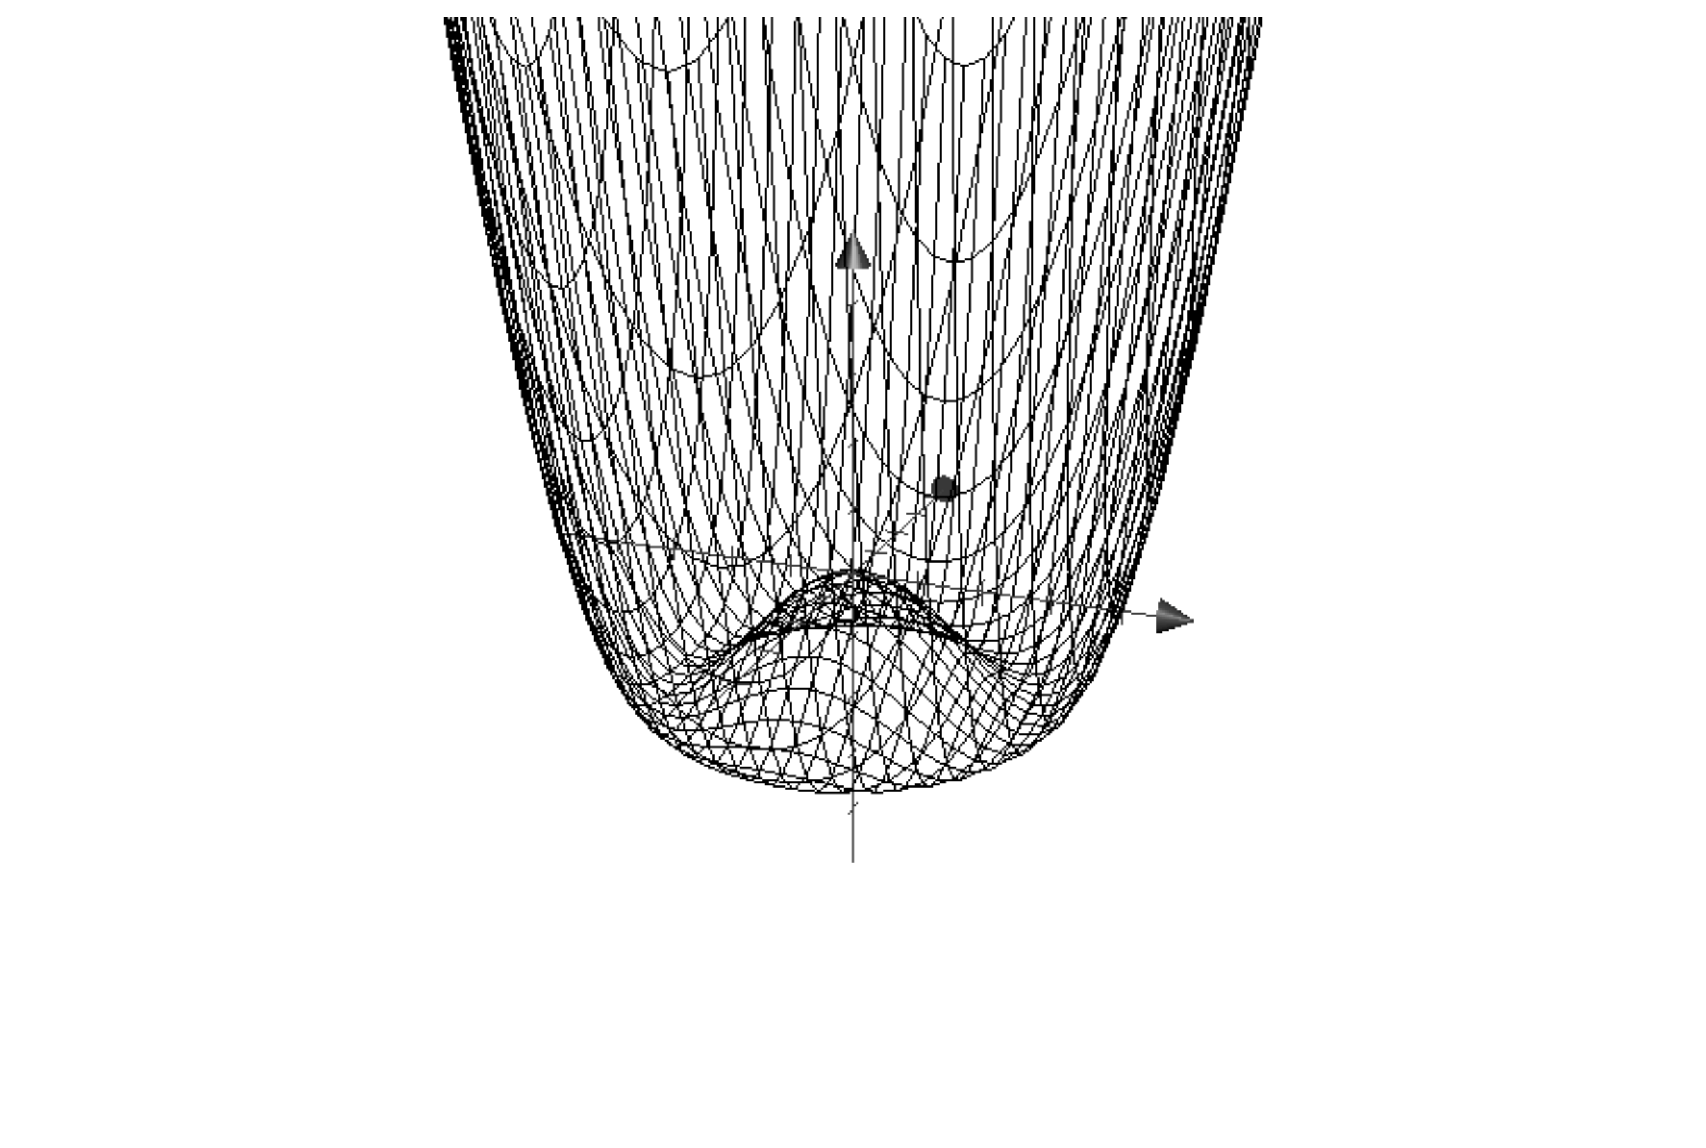
\includegraphics[width = 10cm]{Pictures/SM/mexHat.eps}
      \caption{Higgs potential $V(\phi)$ for $\mu^2 < 0$.}
      \label{fig:scalarPotential}
      \end{figure}

      \todo{Yukawa couplings with fermions}

  \section{Beyond the Standard Model}

  The \gls{SM} constitutes one of the most successful achievements in modern physics.
  One of its strength is to provide an elegant theoretical framework to describe the known experimental facts about particles, but it is also able to predict the existence of a mechanism to generate the particle masses via the Higgs mechanism.
  Nevertheless, a lot of mysteries in the Universe are not explained by this theory. 
  
    \subsection{Limitations of the Standard Model}

    Despite the fact that the experimental results are in good agreement with the \gls{SM} predictions, this theory does not provide answers to may questions.
    The particle physics community tries to unify theories.

      \subsubsection{Free parameters}

      Up to 19 free parameters are used in the \gls{SM} and this theory does not explain their existence.
      Even if it is not as major problem for the physics itself, the particle physics community has a lack of understanding and explaining these values.
      The free parameters are: 
      \begin{itemize}
        \item the masses of the nine fermions,
        \item the coupling constants $g$ and $g'$ of the $U(1)$, $SU(2)$ groups,
        \item the coupling constant of the strong interaction $\alpha_s$,
        \item the three mixing angles, as well as the CP-violating phase of the CKM matrix,
        \item the Higgs boson mass and the expected vacuum value for the Higgs field $vev$,
        \item $\theta^{\rm{QCD}}_{\rm{CP}}$, a parameter that allows the CP violation in \gls{QCD}.
      \end{itemize}

      To this 19 free parameters, 7 other parameters can be considered, thus increasing the number of parameters to 26.
      This parameters are the masses of the three neutrinos, as well as the four parameters of the \textit{Pontecovro-Maki-Nakagawa-Sakata} matrix\footnote{equivalent of the CKM matrix for the neutrinos' mass}.
    
      \subsubsection{Hierarchy problem}

      The hierarchy problem refers to two main energy scales problem of the \gls{SM}.

      First of all, the difference between the energy scale of the \gls{SM} and the Planck scale is of seventeen orders of magnitude.
      No "intermediate" physics has been found between the two scales.

      A second problem occurs while considering the Higgs boson mass.
      The \gls{SM} does not predict its mass, but it sets some theoretical bounds with respect to $\Lambda$, the energy scale at which the \gls{SM} is not valid anymore.
      The theoretical Higgs boson mass is higher than what it should be compared to the EW scale.
      The Higgs boson interacts with the particles of the \gls{SM} (fermions, $W$ and $Z$ boson), but it also interacts with itself.
      Due to the scalar nature of the boson, there are quartic divergences while calculating the loop corrections.
      The quantum corrections, which take into account the coupling of the Higgs boson, are $\Lambda^2$ divergent and lead to a huge Higgs boson mass.
      To avoid that, delicate cancellations should occur between the quantum corrections.
      These cancellations are known as the fine-tuning problem. 
      
      \subsubsection{Gravitation}

      Although particle physicists are dreaming of a "theory of everything" that will unify the electroweak, strong and gravitational interactions, there is no viable theory to describe the gravity in a quantum point of view to include it in the \gls{SM} and which would be still valid at a macroscopic scale.

      \subsubsection{Neutrino mass}

      The neutrinos defined by the \gls{SM} are assumed to be exactly massless.
      Nevertheless at the end of the year 1990, the Super Kamiokande experiment had surprising results \cite{Super-Kamiokande-Oscillation}.
      The measured flux of solar and atmosphere neutrons was lower than expected.
      The result was interpreted by an oscillation of neutrinos between the three leptonic flavors.
      However, the oscillation is possible only if the neutrino has a mass.
      That phenomenon could be considered as a proof of physics beyond the \gls{SM}.

      \subsubsection{Matter-antimatter asymmetry}

      As discussed at the beginning of this chapter, the \gls{SM} defines an equal number types of particles and anti-particles. 
      In the case of the Big Bang theory, it is assumed that the matter and antimatter were created in an exactly equal amount, but a mechanism has favoured electrons, protons, and neutrons with respect to positrons, antiprotons and antineutrons.
      If the amount of matter and antimatter was equal, our Universe would have been completely annihilated.
      The matter domination could be a local phenomenon with an antimatter surrounding the region. 
      However, the region of contact between matter and antimatter would be a violent place of interaction, which would disturb the cosmic microwave background.

      An assumption to explain the asymmetry is that the antimatter was produced in an infinity proportion compared to the matter.
      Hence, the annihilation as lead to create a Universe only made of matter.
      A mechanism which tends to prefer the matter has been observed in the study of the kaon oscillation.
      This particle is able to transform spontaneously to its own anti-particle and vice-versa.
      Nevertheless, this transformation is not symmetric: the kaon is slower to turn into an anti-kaon than the inverse transformation.
 
      \subsubsection{Dark Matter and dark energy}
      
     % \todo{Rephrase dark matter and dark energy}
      Several astrophysical observations are indicating that the Universe is made not only of visible matter but also of matter that seems to be invisible to the electromagnetic interaction and is called the dark matter.
      In 1933, a measurement of the galaxies velocities in the Coma cluster to determine the cluster mass gives a surprising result.
      The mass was more than two orders of magnitude bigger than the mass of visible stars in the cluster.
      It was found that the matter of the \gls{SM} describes only $5~\%$ of the Universe content. 
      The rest of the Universe is made of $22~\%$ of dark matter and around $73~\%$ of dark energy.
      The neutrinos are possible candidates to dark matter, as they couple to \gls{SM} matter only via weak interaction, but they cannot account for the entire density of the universe.
      Nowadays only twelve particles (plus the anti-particles associated) have been observed. 

    \subsection{Theories beyond the Standard Model}

      \subsubsection{Supersymmetry}
    
      The \gls{SUSY} is a \gls{QFT}, that relates the elementary fermions known to corresponding bosons, called sfermions and the bosons to corresponding fermions, called sbosons \cite{Signer2009}.
      The new particles introduced are called super-partners.
      They have the same mass, the same quantum numbers but the spin is differing by a half factor.
      \gls{SUSY} is a broken symmetry. 
      This will allow the super-particles to acquire very high masses.

      \gls{SUSY} is a good candidate for physics beyond the \gls{SM}, as it could solve the hierarchy problem without any fine tuning.
      For example, the loop contributions of one particle to the Higgs are cancelled by the loop contributions of its super-partner.
      It would be able to provide a framework for the unification of the three gauge interactions at a GUT scale.
      The lightest super-particle is a good candidate for the Dark Matter.

      Despite it will answer many questions from the \gls{SM}, there is a lack of understanding why \gls{SUSY} is a broken symmetry.
      
      \subsubsection{Grand unification theory}
      
      After the success of the electroweak unification, the next step is to include the strong interaction to build the \gls{GUT}, an extension of the \gls{SM}.
      In this framework, the three forces are different manifestations of a single interaction. 
      It includes the $\rm{SU}(3)_{\rm{C}} \otimes \rm{SU}(2)_{\rm{L}} \otimes \rm{U}(1)_{\rm{Y}}$ symmetry group into a larger $\rm{SU}(5)$ group. 
      The quarks and leptons are ordered in left-handed decuplets and right-handed quintets.
      The coupling constants are described by only one parameter.  
      There are 24 mediators, the 12 mediators of the \gls{SM} plus 6 $X$ mediators (charge $\pm4/3$ and 3 colors) and 6 $Y$ mediators (charge $\pm1/3$ and 3 colors).
      It predicts the existence of new particles as leptoquarks\footnote{Coupling between a lepton and a quark}, multiple Higgs bosons and new currents.

      Unfortunately, the theory is not validated because of its prediction of the proton lifetime. 
      The first \gls{GUT} was introduced by Georgi and Glashow in 1974 and predicted the decay of the proton \cite{Georgi:1974sy}. 
      The actual experimental limit of the proton lifetime is of $5 \times 10^{32}$ years, whereas the predicted lifetime defined by the $\rm{SU}(5)$ group is one order of magnitude lower \cite{Agashe:2014kda}.

      \subsubsection{Technicolor}

      The technicolor is a theory that explains the mass generation.
      Contrary to the \gls{EW} symmetry, the masses of particles are not generated by the spontaneous symmetry breaking but they are generated by a strong gauge interaction.
      This interaction is strong and confined at the energy that has been experimentally probed.
      The approach of the theory avoids the hierarchy problem induced by the \gls{SM}.
      
      \subsubsection{String theory}

      The particle physicists have the dream of unifying the forces of the nature to have only one single interaction with four different manifestations.
      The string theory proposes a framework for the "theory of everything".
      The basic unit of matter is no more considered as particles but one-dimensional strings of which particles are various vibrational modes.

      The string theory is a theory of quantum gravity.
      It tries to unify the gravitation to the quantum 
      Extra dimensions of $10-11$ space-time dimensions.
      Possible explanation for the hierarchy problem.

  \section{Conclusions}

  Along this chapter, the successes and limits of the \gls{SM} were discussed.
  The high energy physics community is trying to study as far as possible the limit of the \gls{SM} and is also trying to find some proof of new physics beyond the \gls{SM}.
  The \gls{LHC} at CERN has permitted in 2012 to point out the existence of a Higgs boson.  
  Nevertheless, the beam structure of the LHC is not efficient enough to perform very precise measurements.
  Because of the collision between protons, the energy of the collision can't be exactly known.
  The next chapter deals with a future experiment in high energy physics, where electrons and positrons are used to probe the matter instead of protons and anti-protons.


	  
    \chapter{The future of high-energy physics: the ILC}

 %Introduction on the limits of the LHC and why a new colliding experiment is needed
 % First part: describing the main characteristics of the ILC (energy scale, legnth, luminosity)
 %   -> Design (e+/e- sources, damping ring, main linacs, beam delivery system and interaction region )
 %   -> Beam properties
 %   -> Background: beam-beam interaction (luminosity enhancement ~2 BUT hard bremstrahlung that degrades the energy spectrum), pair background (coherent and incoherent production of e+e-)
 % Second part: Detector
 %   -> Option for two experiments (PUSH-PULL)
 %   -> Main differences between the ILD and the SiD
 %   -> Talking about the ILD (VTX, SIT, TPC, f)


  The LHC has started in 2008. The energy scales reaches by the LHC has permitted the discovery of the Higgs boson, but also a spin-3 particles with the LHCb experiment.
  The LHC was designed to be a really challenging machine with a record centre-of-mass energy of collisions on Earth.
  It consists of ??? kilometer ring that provides collision of 14 TeV. 
  Unfortunately, the collision are not well known due to the structure of the proton. 
  Only an estimation of the energy collision is know and the huge QCD background limit the precision of measurement.
  The LHC is the most powerful tool for direct discovery

  A lepton collider is running at lower energy to perform high sensitivity investigations.
  
  The high energy physics community is thinking about a future accelerator which would work as a complement of the LHC.


  Since the beginning of the 2000, the high energy physics community is thinking about a future accelerator to work in complement of the LHC.


  Two projects are considered for the future: the ILC and CLIC (far future).
  Due to the purpose of this thesis, only the ILC project will be presented. 
  
  
   
  \section{The ILC machine}

  \begin{figure}
    \centering
    \missingfigure{Design of the ILC}
    \caption{Basic design of the International Linear Collider}
    \label{fig:ILC}
  \end{figure}
  \section{The SiD}

  \section{The ILD}


    \chapter{Physics at the ILC}
\label{chap:phyics}

  In chapter~\ref{chap:SM}, the framework of particles physics was described. 
  Since the beginning of the high-energy physics, different experiments have been performed to confirm the exactness of the \acrfull{SM} and to try to find traces of new physics beyond the \gls{SM}.
  Depending on the type of colliders used, the measurements do not achieved the same precision. 
  %The beam structure of the different colliders allow to perform different measurements with different precision. 
  For example, the \gls{LHC} with its high luminosity and high energy beam, is able to reach new energy scales, whereas the \gls{ILC} with its electron/positron interaction at lower energy beam is able to perform more precise measurements, due to the known initial state and the free \gls{QCD} background. 
  Along this chapter, the physics scenarios that are scheduled at the \gls{ILC} are discussed. 
  Afterward, the emphasis will be on the Higgs physics and the measurement that would be performed at the \gls{ILC}. 
  The last section aims to introduce a physics analysis scenario to study the processes leading to a Higgs boson and two neutrinos in the final state.
 
 \minitoc

  \section{Potential studies}

  As seen in chapter \ref{chap:ILC}, the \gls{ILC} will have a vast and variable tunable centre-of-mass energy.
  Due to the features of an $e^-e^+$ collider, there is no contribution from strong interaction background and the initial state of collision is well defined, contrary to the \gls{LHC}.
  Moreover, the electroweak background is calculable and controlled.
  All the conditions are reunite to perform precise physics measurements and to look for an evidence of new physics beyond the \gls{SM}.
  The different measurements which will be performed are presented below.

   First of all, a study of the $Z$ boson at the centre-of-mass energy of $\sqrt{s} = 91~\rm{GeV}$ around the $Z$ resonance is scheduled. 
   This program called \textit{GigaZ} will be able to collect more $Z$ boson events than the Large Electron Positron collider (LEP) did, because of a luminosity two to three times higher than what was achieved. 
   The data collected will allow a study on the asymmetries of the $Z$ boson couplings. 
   A second program, called \textit{MegaW}, will be performed at the centre-of-mass energy of $\sqrt{s} = 160~\rm{GeV}$ reaching the $WW$ production threshold and trying to measure the $W$ boson mass with a precision of $\rm{MeV/c}^2$.
   At higher energy, it will also be possible to measure more precisely the $W$ boson couplings.

   Afterward, the centre-of-mass energy will be adjusted to $\sqrt{s} = 250~\rm{GeV}$ to perform a study on the Higgs boson couplings, as well to measure the quantum numbers associated to the boson.
   At this energy, the Higgs boson is mainly procduced via Higgs-strahlung.
   The measurement is done thanks to the recoil mass independently of the Higgs decay products.
 
   Then, for a centre-of-mass energy between 350 and 400 GeV, two studies are achievable. 
   The $WW$-fusion process starts to rise and permits to measure the couplings of the Higgs boson to the $W$ ones in order to look for deviation from the Standard Model. 
   Moreover, this channel allows to study some rare decays. 
   This energy range corresponds also to the threshold of the top quark pairs production.
   Due to the top quark life-time, the two quarks created are not in a bounded-state.
   By performing a threshold scan, the mass of the top quark can be measured with a precision reaching 100 $\rm{MeV/c}^2$.

   The nominal energy of the \gls{ILC} is achieved at $\sqrt{s} = 500~\rm{GeV}$.
   This energy scale is suitable to look for supersymmetry candidates and possible extended states of the Higgs boson.

   An upgrade of the ILC to reach the centre-of-mass energy $\sqrt{s} = 1~\rm{TeV}$ is also scheduled.
   Up to 1 TeV, new measurements are possible, such as the coupling of the Higgs boson to the top quark, the Higgs boson self-coupling, or its compositeness.
   Although, search for new exotic particles and physics beyond the \gls{SM} is possible.
    
   The table~\ref{tab:physicsAtIlc} summarises the different physics programs at the \gls{ILC} for the different energy reachable.  

  \begin{table}[h]
    \begin{center}
    \begin{tabular}{c c c}
      \hline %----------------------------
      Energy (GeV) &  Reaction  &  Physics Goal \tabularnewline
      \hline %----------------------------
      \hline %----------------------------
      91  &  $e^+e^- \rightarrow $Z$ $ & ultra-precision electroweak \tabularnewline
      \hline %----------------------------
      160 & $e^+e^- \rightarrow WW $ & ultra-precision $W$ mass \tabularnewline
      \hline %----------------------------
      250 & $e^+e^- \rightarrow Zh$ & precision Higgs coupling \tabularnewline
      \hline %---------------------------- 
      \multirow{3}*{350 - 400} & $e^+e^- \rightarrow t\overline{t}$ & top quark mass and couplings \tabularnewline
                               & $e^+e^- \rightarrow WW $ & precision $W$ couplings \tabularnewline
                               & $e^+e^- \rightarrow \nu\overline{\nu}h$ & precision Higgs couplings\tabularnewline
      \hline %----------------------------
      \multirow{5}*{500} & $e^+e^- \rightarrow f\overline{f}$ & precision search for Z' \tabularnewline
                         & $e^+e^- \rightarrow t\overline{t}h $ & Higgs coupling to top \tabularnewline
                         & $e^+e^- \rightarrow Zhh $ & Higgs self-coupling \tabularnewline
                         & $e^+e^- \rightarrow \tilde{\chi}\tilde{\chi} $ & search for supersymmetry  \tabularnewline
                         & $e^+e^- \rightarrow AH, H^+ H^-$ & search for extended Higgs states \tabularnewline
      \hline %----------------------------
      \multirow{4}*{700 - 1000} & $e^+e^- \rightarrow \nu\overline{\nu}hh$ & Higgs self-coupling\tabularnewline
                              & $e^+e^- \rightarrow \nu\overline{\nu}VV$ & composite Higgs sector\tabularnewline
                              & $e^+e^- \rightarrow \nu\overline{\nu}t\overline{t}$ & composite Higgs and top\tabularnewline
                              & $e^+e^- \rightarrow \overline{t}\overline{t}^*$ & search for supersymmetry\tabularnewline
      \hline %----------------------------
    \end{tabular}
    \end{center}
      \caption{Summary of the major processes that will be studied at the ILC for different energies \cite{Baer2013}.}
      \label{tab:physicsAtIlc}
  \end{table}
  
  \section{Higgs physics}

  The Higgs boson found at the \gls{LHC} has to be characterised more precisely.
  One of the goal study at the \gls{ILC} is to determine if the particle found is compatible with the one defined by the Standard Model, or if other states exist.
  The measurement of the Higgs boson couplings to the Standard Model particles is one of the key to verify the exactness of the mass generation mechanism described by this theory and to open the door to any proof of physics beyond the Standard Model.
  The production, the decay modes of the Higgs boson, as well as the measurement feasible are presented below in the case of the \gls{ILC}.

    \subsection{Production of the Higgs at the ILC}

    Due to the beam structure at the \gls{ILC}, the Higgs boson is accessible by direct measurement.
    The production of the Higgs boson defined by the Standard Model is done via three major processes: the Higgs-strahlung (see figure~\ref{fig:higgsStrahlung}), the $WW$-fusion (see figure~\ref{fig:WW-fusion}) and the $ZZ$-fusion (see figure~\ref{fig:ZZ-fusion}).

    \begin{description}
      \centering
      \item[Higgs-strahlung:] $e^+e^- \rightarrow ZH \rightarrow f\overline{f}X$
      \item[$WW$-fusion:] $e^+e^- \rightarrow \nu_{e} \overline{\nu_{e}} W^+W^- \rightarrow \nu \overline{\nu} H$
      \item[$ZZ$-fusion:] $e^+e^- \rightarrow e^+e^- ZZ \rightarrow e^+e^- H$
    \end{description}

   % The figure~\ref{fig:higgsProduction} summarises the different Feynman diagrams of the Higgs boson production.

    At the centre-of-mass energy $\sqrt{s} = 250~\rm{GeV}$, the Higgs-strahlung is the dominant process and occurs via a s-channel. 
    Its cross-section falls off as 1/s as the centre-of-mass energy $\sqrt{s}$ increases.
    Contrary to the Higgs-strahlung, the $WW$-fusion and the $ZZ$-fusion are t-channel processes which have a cross-section growing logarithmically with the centre-of-mass energy.
    Thus, at $250~\rm{GeV}$, the cross-section of the $WW$-fusion is one order smaller than the Higgs-strahlung and the $ZZ$-fusion is negligible.
    Nevertheless, around $500~\rm{GeV}$, the $WW$-fusion and the Higgs-strahlung have the same cross-section, which is around 120 fb.
    The figure~\ref{fig:higgsXsec} shows the cross-section production of the Higgs at the ILC regarding the energy of the collision.
    
    \begin{figure}  
        \centering
        \begin{subfigure}[t]{0.3\textwidth}
            \includegraphics[width = 0.9\textwidth]{Pictures/Higgs/Chapter_Theory_figs_ZHdiagram.png}
            \caption{Higgs-Strahlung}
            \label{fig:higgsStrahlung}
        \end{subfigure}
        ~%\qquad
         %add desired spacing between images, e. g. ~, \quad, \qquad, \hfill etc. 
          %(or a blank line to force the subfigure onto a new line)
        \begin{subfigure}[t]{0.3\textwidth}
            \includegraphics[width = 0.9\textwidth]{Pictures/Higgs/Chapter_Theory_figs_nunuHdiagram.png}
            \caption{$WW$-fusion}
            \label{fig:WW-fusion}
        \end{subfigure}
        ~%\qquad
         %add desired spacing between images, e. g. ~, \quad, \qquad, \hfill etc. 
          %(or a blank line to force the subfigure onto a new line)
        \begin{subfigure}[t]{0.3\textwidth}
            \includegraphics[width = 0.9\textwidth]{Pictures/Higgs/HiggsProd_eeH.png}
            \caption{$ZZ$-fusion}
            \label{fig:ZZ-fusion}
        \end{subfigure}
        \caption{Feynman diagrams of the main Higgs production at the ILC \cite{Asner2013}\cite{tian}.}
        \label{fig:higgsProduction}
    \end{figure}    
    
    The $WW$-fusion occurs only with left-handed electrons associated to right-handed positrons.
    Thus, by modifying the beam's polarisation, the signal mixture can be changed, as well as the background processes.

    \begin{figure}[!h]
      \centering
      \includegraphics[width = 0.65\textwidth]{Pictures/Higgs/higgs_xsec_P-8_3.png}
      \caption{The cross section production of the Higgs boson with a mass of 125 GeV \cite{Asner2013}.}
      \label{fig:higgsXsec}
    \end{figure}

    \begin{figure}[!h]
      \centering
      \includegraphics[width = 0.7\textwidth]{Pictures/Higgs/BRTotalUncertBands_lm.png}
      \caption{The Higgs branching ratio with the branching ratio uncertainties for the Higgs mass varying from 80 to 200 GeV \cite{Denner:2011mq}.}
      \label{fig:higgsProd}
    \end{figure}

%    \subsection{Decays of the Higgs}
%    
%    Although the decay $H \rightarrow b\overline{b}$ is the dominant decay mode of the Higgs at hadrons colliders, the existence of the boson was observed by studying the di-photons channel.
%    \todo{H decays at LHC: bb, WW, tau tau, gamma gamma, gg and ZZ}
%    %The Higgs boson discovered at the \gls{LHC} was observed by studying its decay to two photons.
%    %At the \gls{LHC}, the decay $H \rightarrow b\overline{b}$ is observed under special kinematics. 
%    The other decay states are challenging to separate from the background.
%    The properties of the \gls{ILC} beam allow to perform measurements of the Higgs couplings to the particles defined in the \gls{SM}.
%    Thus, the following decay modes are available: $b\overline{b}$, $WW$, $ZZ$, $gg$, $c\overline{c}$, $\tau \tau$, $\gamma \gamma$, $\gamma Z$.
%    The observation of the $H \rightarrow c\overline{c}$ is one of the constraint parameter to build the detectors, specifically, the vertex detector that should be able to distinguish the vertices coming from the $b$-quarks to the ones coming from the $c$-quarks.
%    The figure~\ref{fig:coupling} depicts the mass-coupling relation of the Higgs boson to the particles of the \gls{SM}.
%    Any deviations from the Higgs fermionic coupling would indicate multiple states for the Higgs boson.\todo{Not clear enough}
%%    The study of the Higgs fermionic coupling is a good test to know the nature of the Higgs.
%%    The \gls{SM} nature of the Higgs boson will be tested by looking for any deviations from its fermionic coupling.
%%    A deviation might indicate multiple states for the Higgs boson. \todo{Not clear enough}
%
%    \begin{figure}[!h]
%      \centering
%      \includegraphics[width = 0.5\textwidth]{Pictures/Higgs/Chapter_Theory_figs_mass-coupling1TeV.png}
%      \caption{Mass-coupling relation of the Higgs boson to the particles defined in the standard model\cite{tian}.}
%      \label{fig:coupling}
%    \end{figure}

    \subsection{Higgs studies}

    This section gives few ideas of possible Higgs physics studies.

    \subsubsection{Mass measurement}

    The first study will be at the peak production of the Higgs-strahlung. 
    The well defined four-momentum initial state allows to measure the Higgs boson mass regardless its decay products.
    The Higgs invariant mass $M_H$ can be calculated by using the recoil technique:

    \begin{equation}
      M^2_H = s + M^2_Z - 2 \sqrt{s}\left(E_{1} + E_{2}\right),
    \end{equation}

    where $M_Z$ is the mass of the $Z$ boson, $E_1$ and $E_2$ are the energy of the $Z$ decay products. 
    This technique works well for the $Z$ boson decaying into leptons at the centre-of-mass energy $\sqrt{s} = 250~\rm{GeV}$.
    However, this method can not be performed for a Higgs decaying into quarks at the same energy. 
    The $Z$ and the Higgs bosons are produced almost at rest, thus, the identification of the jets coming from the $Z$ boson to the ones coming from the Higgs is more difficult.
    Nevertheless, at higher energy ($\sqrt{s} = 500~\rm{GeV}$), the two bosons are enough boosted to separate their jets and then to apply again the recoil mass.
    Depending on the decay channel of the $Z$ boson, the statistical precision on the mass measurement varies between 40 MeV (for $Z \rightarrow \mu^+\mu^-$) to 80 MeV (for $Z \rightarrow e^+e^-$) and can reach 32 MeV by combining the two results.

    \subsubsection{Spin measurement}

    At the thresholds production of the Higgs-strahlung ($\sqrt{s} = 250~\rm{GeV}$), besides the mass measurement, the determination of the spin and the CP-violation are scheduled.
    From the \gls{LHC} analysis, it has been determined that a spin-1 Higgs boson is forbidden because of the di-photon channel observation \cite{TheATLASCollaboration2013}.
    The spin will be determined by studying the Higgs-strahlung production mode.
    Indeed, the cross-section has different behaviour, depending on the spin and the CP-violation.
    For a spin-0 and CP-even Higgs boson, the production cross-section follows $s$, whereas for CP-odd, it has a $\sqrt{s}^3$ dependency.

    \subsubsection{Branching ratio measurement}

    Although the decay $H \rightarrow b\overline{b}$ is the dominant decay mode of the Higgs at hadrons colliders, the existence of the boson was observed by studying the di-photons channel.
    \todo{H decays at LHC: bb, $WW$, tau tau, gamma gamma, gg and ZZ}
    %The Higgs boson discovered at the \gls{LHC} was observed by studying its decay to two photons.
    %At the \gls{LHC}, the decay $H \rightarrow b\overline{b}$ is observed under special kinematics. 
    The other decay states are challenging to separate from the background.
    The properties of the \gls{ILC} beam allow to perform measurements of the Higgs couplings to the particles defined in the \gls{SM}.
    Thus, the following decay modes are available: $b\overline{b}$, $WW$, $ZZ$, $gg$, $c\overline{c}$, $\tau \tau$, $\gamma \gamma$, $\gamma Z$.
    The observation of the $H \rightarrow c\overline{c}$ is one of the constraint parameter to build the detectors, specifically, the vertex detector that should be able to distinguish the vertices coming from the $b$-quarks to the ones coming from the $c$-quarks.
    The figure~\ref{fig:coupling} depicts the mass-coupling relation of the Higgs boson to the particles of the \gls{SM}.
    Any deviations from the Higgs fermionic coupling would indicate multiple states for the Higgs boson.\todo{Not clear enough}
%    The study of the Higgs fermionic coupling is a good test to know the nature of the Higgs.
%    The \gls{SM} nature of the Higgs boson will be tested by looking for any deviations from its fermionic coupling.
%    A deviation might indicate multiple states for the Higgs boson. \todo{Not clear enough}

    \begin{figure}[!h]
      \centering
      \includegraphics[width = 0.5\textwidth]{Pictures/Higgs/Chapter_Theory_figs_mass-coupling1TeV.png}
      \caption{Mass-coupling relation of the Higgs boson to the particles defined in the standard model \cite{tian}.}
      \label{fig:coupling}
    \end{figure}


 
    %Complementary test at the centre-of-mass energy $\sqrt{s} = 250~\rm{GeV}$ will be conducted to measure the spin and the CP-violation.
    %The \gls{LHC} analysis has permit to exclude a spin-1 Higgs boson with the observation of di-photon events.
    %%Indeed, this energy corresponds to the thresholds production of the Higgs-strahlung. 
    %Depending on the spin and the CP-violation, this production mode has different behaviors.
    %For a spin 0 and CP-even, the production cross-section follows $s$, whereas for CP-odd, it has a $\sqrt{s}^3$ dependency.

  \section{Analysis of simulated data}
  
    Due to the restricted time to conduct the thesis, this section is introducing the tools to perform an analysis of simulated data at the ILD. 
    The results shown here are not the last update and are already demonstrated \cite{Mueller}. 
    Nevertheless, the philosophy to perform a study of the Higgs production at the center-of-mass energy $\sqrt{s} = 350$ GeV and a luminosity of 250 $\text{fb}^{-1}$ is here presented.
  
  \subsection{Simulation set-up}  
  \label{subsec:ILCSOFT}

    The physics events are generated with Monte-Carlo simulation tools and is performed with different software.
    The collisions of electrons and positrons is done with the software WHIZARD \cite{WHIZARD}.
    It supports the \gls{SM} processes, as well as a large variety of BSM models.
    For linear collider physics, the beamstrahlung, the \gls{ISR} and the beam polarisation are simulated, but the hadronisation and fragmentation are not implemented and the simulation of this events was performed with PYTHIA \cite{PYTHIA}.
  
    The linear collider community has developed Monte-Carlo simulation and analysis software frameworks dedicated for a future linear collider, such as the \gls{ILC}. 
    The different packages developed by the community are grouped into the ILCSoft framework \cite{ilcsoft}.
    %The ILCSoft provides a large variety of software packages which were developed for the linear collider community\cite{ilcsoft}.
    It includes software for Monte-Carlo simulation, as software for test beam analysis (see chapter~\ref{chap:X0}) and other tools.
    The main package is the \gls{LCIO}, a persistence framework and event data model for the linear collider detector studies \cite{lcio}. 
    It provides a common data format and event data model for both the simulation studies and the analysis framework in order to share results and compare reconstruction algorithms.

    %The Monte-Carlo simulation is performed in three steps.
    %The first one consists to generate the physics events of electron/positron collisions.
    %The generation of Mont-Carlo events are performed with WHIZARD\cite{WHIZARD}.
    %This software includes \gls{SM} processes, as well as a large variety of BSM models.
    %For the purpose of the \gls{ILC}, it can simulate the beamstrahlung, the \gls{ISR} and the beam polarisation.
    %Although the hard interaction are simulated with WHIZARD, the hadronisation and fragmentation are implemented by using PYTHIA\cite{PYTHIA}.

    Afterward the physics events are generated, the particle interaction inside the detector is simulated with Mokka \cite{Mokka}.
    The software is based on GEANT4 simulation toolkit \cite{GEANT4} and is part of the ILCSoft.
    For the analysis, the detector model used is ILD\_o1\_v05.
    This model simulates the dead areas due to cabling, cooling system and mechanical structure and has a silicon-tungsten electromagnetic calorimeter, as well as an analog hadronic calorimeter.
    
    The detector geometry is described by a XML steering file and is used as an interface during the data reconstruction and analysis.
    This is managed by the \gls{GEAR} software \cite{GEAR}.

    Finally, the events are reconstructed with the \gls{Marlin} package \cite{MARLIN}.
    It is a C++ software framework used for the data reconstruction and the data analysis and it handles \gls{LCIO} data format.
    The different steps of the analysis or the reconstruction are grouped into modules, also called processors that read an input file, perform the defined tasks and write an output file that could be processes by another \gls{Marlin} module.
    A steering file written in XML is used to select the processors to use and the order of their execution time.

  \subsection{Event generation}
     
     \subsubsection{Event samples}

     The \gls{ILD} generator group has produced signal and background samples for two different polarisations:  $\mathcal{P}_{e^-,e^+} = (-1,+1)$ and $\mathcal{P}_{e^-,e^+} = (+1,-1)$.
     Although the scheduled polarisation are $\mathcal{P}_{e^-,e^+} = (-0.8,+0.3)$ and  $\mathcal{P}_{e^-,e^+} = (+0.8,-0.3)$, the simulated beam polarisation is re-weighted according to:
     
     \begin{equation}
       \begin{array}{lrc}
       \sigma_{\mathcal{P}_{e^-,e^+}} & = & \frac{(1 - P_{e^-})(1+P_{e^+})}{2} \sigma_{LR} + \frac{(1+P_{e^-})(1-P_{e^+})}{2} \sigma_{RL}, \\
       \sigma_{-0.8,+0.3} & = & 0.585 \times \sigma_{LR} + 0.035 \times \sigma_{RL}, \\
       \sigma_{+0.8,-0.3} & = & 0.035 \times \sigma_{LR} + 0.585 \times \sigma_{RL}.
       \end{array}
     \end{equation}

     The cross-section $\sigma_{LR}$ is for the polarisation $\mathcal{P}_{e^-,e^+} = (-1,+1)$, whereas $\sigma_{RL}$ is the cross-section of the polarisation $\mathcal{P}_{e^-,e^+} = (+1,-1)$.
     On the one hand, the Higgs-strahlung and the $WW$-fusion processes are equally important for the beam polarisation  $\mathcal{P}_{e^-,e^+} = (-0.8,+0.3)$, leading to a larger $\nu\overline{\nu} H$ cross-section.
     On the other hand, the polarisation $\mathcal{P}_{e^-,e^+} = (-0.8,+0.3)$ is used to perform a cross-check measurement.
     Indeed, the $W$-boson cannot couple to right-handed electrons and left-handed positrons.
     Thus, the $WW$-fusion process is largely suppressed.
     Besides, the $Z$-boson depends on the isospin and the Higgs-strahlung contribution is also reduced but not suppressed.
     The same effect occurs on the backgrounds leading to a smaller background contamination on the signal and a cleaner signal sample for the Higgs-strahlung.

     The data set are scaled to an integrated luminosity of $250~\rm{fb}^{-1}$ for each beam polarisation.

  \subsubsection{Signal}

    The signal to study is the final state $\nu\overline{\nu}H$, on which the Higgs boson decays into a pair of quarks, such as $H \rightarrow b\overline{b}$ and $H \rightarrow c\overline{c}$, or a pair of gluons $H \rightarrow gg$. 
    The other decay modes are considered here as a source of background. 
    The dominant production processes leading to this final state are the Higgs-strahlung and the $WW$-fusion.
    Their leading order Feynman diagrams are displayed respectively on figure~\ref{fig:higgsStrahlung} and~\ref{fig:WW-fusion}.
    Although the neutrinos produced in the $WW$-fusion process are only $\nu_{\rm{e}}$ and all neutrino flavors are equi-probable in the Higgs-strahlung, the neutrino flavors cannot be detect and only the missing energy is the signature of neutrino production.

    \begin{figure}[!h]
      \centering
      \includegraphics[width = 0.9\textwidth]{Pictures/Higgs/mMiss.png}
      \caption{Distribution of the missing mass with different beam polarisations and for the Higgs-strahlung and $WW$-fusion leading to $\nu\overline{\nu}H$ final state.
      The background contribution is not taken into account here.}
      \label{fig:mMiss}
    \end{figure}

    The figure~\ref{fig:mMiss} represents the distribution of the missing mass for the signal events for the two polarisations considered at the \gls{ILC}.
    The first effect of the polarisation is the suppression of the $WW$-fusion contribution and also a reduction of the Higgs-strahlung for right-handed electrons and left-handed positrons.
    For the other polarisation, the missing mass distribution shows three peaks. 
    Once centered around $90~\rm{GeV}$ corresponding to the decay of the Z-boson into a pair of neutrinos.
    The second peak is broader and its maximum is at $200~\rm{GeV}$.
    This comes from the $WW$-fusion.
    A third peak is visible at $300~\rm{GeV}$ and is coming from the Higgs boson decaying not hadronically and is considered as a source of background.    

  \subsubsection{Background processes}

    The signal hypothesis is that the final state is consisting of two jets coming from the hadronic decay of the Higgs boson, as well as missing energy coming from the undetected neutrinos produced by the $Z$ boson decay.
    Nonetheless, this signal is drown into the background processes.
    The background consists to the events with the same final states as the signal, called irreducible background and the events with a similar detector response.
    Their contributions depend on the beam polarisation.
    For example, the cross-section for a beam polarisation $\mathcal{P}_{e^-,e^+} = (+0.8,-0.3)$ is smaller by an order of magnitude due to the $W$ boson.

    Two irreducible backgrounds are considered here, the one involving a $W$-boson exchange and the one with a $Z$-boson exchange.
    The cross-section of this processes is few times larger than the signal one.
    For both, single $W$-boson and $Z$-boson exchange, the final state contains two jets with missing energy.
    Nevertheless, the final state with quarks is more likely than the final state with two gluons due to the loop formed in the final state on which the gluons are emitted.

    The background involving $W$-bosons, such as $e^{-}e^{+} \rightarrow W^{\pm}e^{\pm}\nu_{e} \rightarrow e^{\pm}\nu_{e}q\overline{q}$ is two orders magnitude bigger than the signal cross-section.
    The neutrino produced carries a large transverse momentum, whereas the electron or positron has a low transverse momentum.
    Hence, it can be undetected and be considered as a missing energy.
    
    The $W$-pair production can lead to semi-leptonic, hadronic and leptonic decay modes.
    The semi-leptonic mode consists of two jets and a lepton with its associated neutrino ($e^{+}e^{-} \rightarrow W^+W^- \rightarrow \nu_{l}l^{\pm}q\overline{q}$) and it is the major background process for the $W$-pair production.
    This background is detected by looking for an isolated lepton.
    Nevertheless, the lepton could escape the detector undetected or be inside a jet.
    The second $W$-pair production is the hadronic decay on which there is no missing energy ($e^{+}e^{-} \rightarrow W^+W^- \rightarrow q\overline{q} q\overline{q}$).
    This background is reduced by applying cuts on the missing momentum and the di-jet invariant mass.
    The last contribution is the leptonic final state, which is easy to distinguish from the signal.
    Thus, it is not considered in the study. 

    The $Z$-pair background is ten times smaller than the $W$-pair production.
    The  $e^+e^- \rightarrow ZZ \rightarrow \nu_{l}\overline{\nu_{l}}q \overline{q}$ process is an irreducible background.
    The hadronic decay $e^+e^- \rightarrow ZZ \rightarrow q\overline{q} q\overline{q}$ is reduced by cutting on the missing momentum and the di-jet invariant mass.
    The semi-leptonic process $e^+e^- \rightarrow ZZ \rightarrow l^+l^- q\overline{q}$ is easier to detect because of the second isolated lepton in the event.

    Finally, the last background to take into account is the one with the Higgs boson produced in the final state.
    The Higgs-strahlung can lead to $q\overline{q}H$ and $l^{\pm}l^{\mp}H$ has cross-section three times larger than the signal, but it is easily identify due to the absence of neutrino.
    All the decay mode of the Higgs different from $H \rightarrow b\overline{b}$, $H \rightarrow c\overline{c}$ and $H \rightarrow gg$ are considered as part of the background.

    \begin{figure}[!h]
      \centering
      \includegraphics[width = 0.9\textwidth]{Pictures/Higgs/mVis_all.png}
      \caption{Distribution of the visible mass for the signal and background together and the polarisation $\mathcal{P}_{e^-,e^+} = (-0.8,+0.3)$.}
      \label{fig:mVisAll}
    \end{figure}

    The figure~\ref{fig:mVisAll} displays the distribution of the visible mass for all the processes taken into account during the analysis and a beam polarisation $\mathcal{P}_{e^-,e^+} = (-0.8,+0.3)$.
    A selection has to be performed in order to isolate the peak at $125~\rm{GeV}$.

  \section{Results}
 
    \subsection{Event reconstruction}

    The assumption to study the $H \nu\nu$ channel is to reconstruct a final state which is giving a two jets and missing energy in the detector response.
    The reconstruction consists to select and highlight this detector response.

    The first step consists to identify in the events the presence of isolated leptons in the final state and to remove them from the physics list.
    The lepton detected outside a jet are considered as a source of background.
    Thus, a neural network is used to identify in an event the different leptons and checks if they belong to a jet.
    This selection is based on different criteria, like the vertex information, the energy deposited inside the \gls{ECAL}, the \gls{HCAL} and the muon system. 
    The processor used for the identification is called \textit{IsolatedLeptonTagger} and has a veto efficiency of roughly $90~\%$.
    The $10~\%$ of leptons undetected are coming from events in which the leptons are moving into the forward region and they could escape the detector without being identify by the processor.
    A better selection is done after the jet reconstruction and is discussed later.

    A second source of background is coming from the $\gamma \gamma$ interactions which produce low $p_{t}$ hadrons.
    This hadrons with a small transverse momenta and a small relative angle to the beam axis are detected as jet-like objects in the forward region of the detector.
    The identification of the beam jets is based on the $k_{T}$ algorithm \cite{Cacciari2008}.
    It consists to define a "distance" $d_{ij}$ between two particles and to find the first closest constituent.
    
    \begin{equation}
      \begin{array}{lcl}
        d_{ij} & = & \frac{\rm{min}\left(p^2_{T_i}, p^2_{T_j}\right) \cdot \Delta R^2_{ij}}{R^2}, \\
        d_{i}  & = & p^2_{T_i},
      \end{array}
    \end{equation}

    with $\Delta R^2_{ij} = \left( y_{i} - y_{j}\right)^2 + \left( \phi_{i} - \phi_{j}\right)^2$, $y_{i}$ the pseudo rapidity, $\phi_{i}$ the azimuthal angle and $p_{T_i}$ the transverse momentum of the particle studied.
    The minimum between $d_{ij}$ and $d_{i}$ is calculated.
    If $d_{ij}$ is the minimum value, then, the particles $i$ and $j$ are merged into a jet candidate, they are then removed from the physics list and the jet candidate is added instead.
    If the minimum value is $d_{i}$, the particle is considered to be part of the beam jet and is removed from the particle lists.
    This algorithm is repeated iteratively until the number of jets created is equal to the number of jets expected.
   
    After removing the isolated leptons and the low $p_{t}$ hadrons from the physics list, the jet clustering and the flavor tagging processors are applied. 
    Because of the $k_{T}$ algorithm, which removes particle from the physics list, the vertex finder is run again before to use the jet clustering algorithm.

  \subsection{Event selection}

  To improve the signal to noise ratio, an event selection is performed by applying different cuts that reduce the background contribution.
  The order and the performances of the selection cuts are determined by maximising the significance $s$, which is:

  \begin{equation}
    s = \frac{\rm{N_{sig}}}{\sqrt{\rm{N_{sig}}+ \rm{N_{bg}}}},
  \end{equation}

  with, $\rm{N_{bg}}$ the number of remaining background and $\rm{N_{sig}}$, the number of remaining signal.
  The maximisation of $s$ is needed to minimise the statistical error.
  Firstly, the procedure starts with the definition of a collection of observables that could help to discriminate the signal from the background.
  Then, a test of the possible cut values is performed in a given range and for a given step size.
  The value leading to the largest significance is chosen as the optimum observable and is the first selection variable which is applied to a signal sample (containing $WW$-fusion and Higgs-strahlung processes) and the least tight constraint is selected in order to maintain a good signal efficiency.
  Finally, the cut values of this optimum observable is applied on the complete data set and the procedure is applied again.

  The first observable to be applied is the veto information used to find any isolated lepton.
  As already mentioned, the \textit{IsolatedLeptonTagger} processor has a veto efficiency of roughly $90~\%$. 

  The second observable is the visible transverse momentum $P_{\rm{t,vis}}$ of the di-jets. 
  \begin{equation}
    \begin{array}{lcl}
      P_{\rm{t,vis}} = \sqrt{P^2_{x,vis} + P^2_{y,vis}}, \\
      P_{\rm{x/y,vis}} = P_{\rm{x/y,j1}} + P_{\rm{x/y,j2}}. 
    \end{array}
  \end{equation}
 
  $ P_{\rm{x/y,j1}}$ and $ P_{\rm{x/y,j2}}$ are the visible momentum in the $x$ and $y$-directions for the two jets $j1$ and $j2$.

  The third observable is the invariant visible mass $m_{\rm{vis}}$, which is the signal signature.

  \begin{equation}
   \rm{m_{vis}} = \sqrt{E^2_{\rm{vis}} - \overrightarrow{P}^{\,2}_{\rm{vis}}},
  \end{equation}

  with $E_{\rm{vis}}$ and $P_{\rm{vis}}$ the visible energy and momentum of the event.
  The expected visible mass is $\rm{m_H} = 125~\rm{GeV}$ and its width is mainly driven by the jet energy resolution.

%    \begin{sidewaystable}
%    \scriptsize{
%    \flushleft
%      \begin{tabular}{c c c c c c c}
%           \hline
%           {Process} & {Cross Section (fb)} & {Events number} & \text{No isolated leptons} & {$35 <~\rm{{P}_{t}^{vis}} < 155~\rm{GeV} $} & {$95 <~\rm{m_{vis}}< 140~\rm{GeV}$} & {$-1 <~\rm{\cos{\alpha}}< 0.22$} \tabularnewline \hline
%           \hline
%           Zhad            &$ 3.86\times 10^{4} $&$	1.27\times 10^{7} $&$ 1.26\times 10^{7} $&$ 1.09\times 10^{5} $&$ 5.79\times 10^{2} $ &$	5.05\times 10^{2}  $\tabularnewline 
%           WW had          &$ 6.53\times 10^{3} $&$	2.16\times 10^{6} $&$	2.14\times 10^{6} $&$	5.27\times 10^{3} $&$	6.29              $ &$	6.29               $\tabularnewline 
%           WW semilep      &$ 8.16\times 10^{3} $&$	2.69\times 10^{6} $&$	1.17\times 10^{6} $&$	6.38\times 10^{5} $&$	1.13\times 10^{5} $ &$  6.26\times 10^{4}  $\tabularnewline 
%           ZZ had          &$ 6.01\times 10^{2} $&$	1.98\times 10^{5} $&$	1.97\times 10^{5} $&$	2.74\times 10^{3} $&$	1.20              $ &$  6.20\times 10^{-1} $\tabularnewline 
%           ZZ semilep      &$ 5.65\times 10^{2} $&$ 1.86\times 10^{5} $&$ 1.40\times 10^{5} $&$ 7.49\times 10^{4} $&$ 1.46\times 10^{4} $ &$  8.20\times 10^{3}  $\tabularnewline 
%           singleW semilep &$ 1.63\times 10^{3} $&$ 5.36\times 10^{5} $&$	2.24\times 10^{4} $&$	8.79\times 10^{3} $&$	1.65\times 10^{3} $ &$	1.63\times 10^{3}  $\tabularnewline 
%           singleZee semi  &$ 3.10\times 10^{2} $&$	1.02\times 10^{5} $&$	1.30\times 10^{4} $&$	2.17\times 10^{1} $&$	7.00\times 10^{-2}$ &$	7.00\times 10^{-2} $\tabularnewline 
%           singleZnn semi  &$ 3.55\times 10^{2} $&$	1.17\times 10^{5} $&$ 1.17\times 10^{5} $&$	8.38\times 10^{4} $&$	1.62\times 10^{4} $ &$	1.19\times 10^{4}  $\tabularnewline 
%           Higgs BG        &$ 1.62\times 10^{2} $&$	5.34\times 10^{4} $&$ 4.19\times 10^{4} $&$ 4.59\times 10^{3} $&$	1.93\times 10^{2} $ &$	1.43\times 10^{2}  $\tabularnewline 
%           HiggsToOther    &$ 3.05\times 10^{1} $&$	1.01\times 10^{4} $&$	6.66\times 10^{3} $&$	4.95\times 10^{3} $&$ 3.45\times 10^{3} $ &$	2.64\times 10^{3}  $\tabularnewline 
%           \hline						
%           Background     &$ 5.69\times 10^{4} $&$  1.88\times 10^{7} $&$	1.65\times 10^{7} $&$	9.31\times 10^{5} $&$ 1.50\times 10^{5} $ &$  8.76\times 10^{4}  $\tabularnewline 
%           Signal	        &$ 6.82\times 10^{2} $&$  2.25\times 10^{4} $&$	2.23\times 10^{4} $&$	1.82\times 10^{4} $&$	1.66\times 10^{4} $ &$	1.57\times 10^{4}  $\tabularnewline 
%           Significance   &                     &$	5.19              $&$	5.48 $             &$	1.87\times 10^{1} $&$	4.06\times 10^{1} $ &$  4.88\times 10^{1}  $\tabularnewline 
%     \end{tabular}
%    }
%    \caption{Cut flow chart with three first cuts applied.}
%    \label{tab:cutFlow}
%  \end{sidewaystable}

  \begin{table}
    \begin{tabular}{c c c c}
      \hline
      Process                                     & Background          & Signal              & Significance  \tabularnewline
      \hline
      \hline
      Cross-section (fb)                          & $5.69 \cdot 10^{4}$ & $6.82 \cdot 10^{2}$ &               \tabularnewline
      \hline
      Expected event number                       & $1.88 \cdot 10^{7}$ & $2.25 \cdot 10^{4}$ & $5.2$         \tabularnewline
      No isolated leptons                         & $1.65 \cdot 10^{7}$ & $2.23 \cdot 10^{4}$ & $5.5$         \tabularnewline
      {$35 <~\rm{{P}_{t}^{vis}} < 155~\rm{GeV} $} & $9.31 \cdot 10^{5}$ & $1.82 \cdot 10^{4}$ & $18.7$        \tabularnewline
      {$95 <~\rm{m_{vis}}< 140~\rm{GeV}$}         & $1.50 \cdot 10^{5}$ & $1.66 \cdot 10^{4}$ & $40.6$        \tabularnewline
      {$-1 <~\rm{\cos{\alpha}}< 0.22$}            & $8.76 \cdot 10^{4}$ & $1.57 \cdot 10^{4}$ & $48.8$        \tabularnewline
      $26 < (\rm{N.R.C > 1GeV}) < 99$             & $2.25 \cdot 10^{4}$ & $1.19 \cdot 10^{4}$ & $56.3$        \tabularnewline
      $0.11 < \rm{DurhamjD2ym} < 1$               & $1.78 \cdot 10^{4}$ & $1.05 \cdot 10^{4}$ & $62.3$        \tabularnewline
      $0 < \rm{abs(RefinedjPzvis)} < 113~\rm{GeV}$& $1.51 \cdot 10^{4}$ & $1.01 \cdot 10^{4}$ & $63.5$        \tabularnewline
      $156 < \rm{RefinedjEmiss} < 230~\rm{GeV}$   & $1.37 \cdot 10^{4}$ & $9.85 \cdot 10^{3}$ & $64.1$        \tabularnewline      
      \hline %----------------------------
    \end{tabular}
    \caption{Cut-flow table for a beam polarisation $\mathcal{P}_{e^{-},e^{+}} = (-0.8, +0.3)$.}
    \label{tab:cutFlow}
  \end{table}

  The table~\ref{tab:cutFlow} summarises the order of the different cut selection for different observables applied on the simulated data set.
  After eight consecutively cuts, the background contribution is three orders smaller, whereas the signal is almost one order smaller than the beginning.
  Nevertheless, the significance is still less than 70 and applying more cuts is affecting strongly the signal.

  \section{Outlooks}

  To preserve the sample quality, it is rather better to use a \gls{MVA} method to extract the signal from the background.
  The complete information is then used simultaneously to find the best sets of variable.
  This analysis was already performed and a \gls{MVA} method was used, achieving a significance above $70$.

  The next step of this analysis is to focus on the decay mode of the Higgs boson into two pairs of charmed quarks and to optimise the flavor tagging performances to separate more accurately the $b$ and $c$ quarks events.
  For the events and the detector simulated in this chapter, the vertex detector geometry was not optimised and was made of five single sided layers.
  Nevertheless, the double sided option has to be investigated.
  This geometry offers multiple possibilities, like using two different types of sensors on the same ladder or the possibility of two point measurements per ladder for a track.
  One side could be equipped with ultra-fast integration time ($\mathcal{O} \sim 1~\rm{\mu s}$) sensors, whereas the other side could embed sensors with an excellent pointing resolution ($\sigma_{\rm{s.p}} \leq 3~\rm{\mu m}$).
  With two sensors on the same mechanical structure, a track is reconstructed by two points of measurement.
  Thus, these two measurements could be combined together to form "mini-vectors".
  Studying the "mini-vectors" could help to identify the beam-strahlung from the collision events.



  %This is important to determine the geometry configuration and the technology used to build the vertex detector.
  %The study could consist first to compare the branching ratio measured with two different detector geometries. 
  %The one used in this analysis was made of a five single sided layers, but to decide which structure, like single or double-sided ladder, the analysis as to be ran again.
  %One possible vertex detector considered is made of three double-sided layers.
  %On one side of a ladder, sensors with an ultra-fast integration time ($\mathcal{O} \sim 1~\rm{\mu s}$) and on the other side, sensors with an excellent pointing resolution ($\sigma_{\rm{s.p}} \leq 3~\rm{\mu m}$).



    \chapter{Double-sided VXD: PLUME}
\label{chap:vxd}

%  The signature of physics interest is essentially done by heavy flavour study.
%  To study the Higgs boson and to understand more precisely the nature of this boson, its coupling with the other \gls{SM} particles is important.
%  The capacity of identifying and being able to reconstruct the decay of t, b, c quarks and $\tau$ leptons is mandatory for a future high energy physics experiment.
%  Contrary to the \gls{LHC}, the vertex detector at the \gls{ILC} should be able to distinguish the c quark from the b quark.
%  This chapter deals with the requirements for a vertex tracker able to extrapolate particle tracks back to their production.
%  Firstly, the main parameters that lead the building of a vertex detector are introduced. 
%  Then, the different options for the \gls{ILD} are shown to focus on the double-sided options developed by the \gls{PLUME} collaboration.
%  To finish, the principle of \gls{CMOS} sensors and their use in physics are described.

  The aim of the \gls{ILC} is to perform precise measurement of new and already known particles. 
  It can be achieved only by a proper detector design, driven by flagship measurements like the Higgs coupling to quarks and bosons.
  In fact, the complex events generated at the \gls{LHC} hide the possibility of a direct measurement of the Higgs.
  The vertex detector at the \gls{ILC} should be able to perform an efficient B-meson tagging and to separate $b$ and $c$ quarks.
  The measurement of heavy quark jets and their decay vertices will play a crucial role in the \gls{ILC} physics.
  Along this chapter, the role of the vertex detector and the physics requirements to build one suited for the \gls{ILC} will be presented.
  Then, the different options for the \gls{ILD} are shown to focus on the double-sided options developed by the PLUME collaboration.
  To finish, the principle of \gls{CMOS} sensors and their use in physics are described.

  Since the 1970's, the development of position sensitive silicon radiation sensors has permit to confirm the prediction of the \gls{SM} with a high precision, as well as the discovery of the $t$ quarks.
  At the \gls{ILC} flagship measurements sch as the Higgs coupling to the quarks and bosons are driving the development of the vertex detector.
  For example, to separate $b$ (1.3 10-12)and $c$ (1.1 10-12)quarks
  To measure particles with a short life-time ($\simeq 10^{12}$s) that have a decay length between 150 and 500 $\mu$m, 


  The sub-detector has to be able to separate particles with a time life $\simeq 10^{-12}$s  


  The \gls{ILC} is aiming to perform more precise measurements of new and already known particles. 

  \minitoc
  
  \section{The ILD vertex detector specifications}
   

    %For the ILD, the resolution at the interaction point should be given by the equation~\ref{eq:resIP}

    %\begin{equation}
    %  \sigma_{IP} = 5 \mu\text{m} \oplus \frac{10 \ - \ 15 \mu\text{m}}{p \sin{\theta}^{3/2} }
    %  \label{eq:resIP}
    %\end{equation}
\todo{Reference : Marco Battaglia - Vertex Tracking at a Future Linear Collider}

    %Where the first term is the impact parameter resolution which depends on the radii of the inner and outer layers and the single point resolution. 
    %In the case of the ILD, the single point resolution should not be higher than $\sigma_{sp} \simeq 3 \mu\text{m}$.
    %The second term is related to the multiple scattering. 

  % \subsection{Role of a VXD}

    Motivations: flavour tagging and life-time measurements via secondary and tertiary vertex finding. 
    To measure lifetime in pico-second regime, on needs spatial resolution of the order of 5-300 microns.
    Typical parameters are thickness, pitch and resolution.
    

    The \gls{VXD} is the closest sub-detector to the \gls{IP} in charge of reconstructing the vertex by extrapolating particles back to their origin of production. 
    This detector should be optimised to track particles in a high density environment and to able to extract the tracks from the different kind of particles, especially the b and c quarks in the case of the \gls{ILC}.
    The reconstruction of the displaced vertices should be efficient enough to perform a good flavour tagging.
    The minimum distance of the first \gls{VXD} layer is determined by the background induced by beamstrahlung.
    This sub-detector has a central role in track reconstruction.
    Depending on the option chosen, the \gls{VXD} has to provide five or six points of measurement with very high precise spatial resolution.
    For the studies requiring vertex charge identification, it should be able to reconstruct low-momentum and very forward tracks.
   

   \subsection{Physics requirements}

   %The design of the \gls{VXD} is constrained by the physics requirement to get an excellent flavour tagging ability.
   %The measurement of the vertex charge and the reconstruction of the displaced vertices is ... 
   The ideal \gls{VXD} should embed sensors with fine granularity to be able to distinguish two nearest particle.
   The structure should be as light as possible to minimize the interaction of particles before their are flying to the other detectors.
   The first layer has to be as close as possible to the \gls{IP} and the lowest power consumption as possible
   The flavour tagging ability, vertex charge measurement and track and displaced vertices reconstruction are the main physics parameter that are driving the design of such detector.
   The distance of closest approach of particle to the colliding beam is called the impact parameter and the resolution achievable by the detector is described by the formula~\ref{eq:resIP}.
   %The resolution on the impact parameter $\sigma_{IP}$, defined as the distance of closest approach of the particle to the colliding beam can be parametrised by the formula~\ref{eq:resIP}.\todo{REPHRASE}
    
    \begin{equation}
      %\sigma_{IP} = 5 \mu\text{m} \oplus \frac{10 \ - \ 15 \mu\text{m}}{p \sin{\theta}^{3/2} }
      \sigma_{IP} = a \oplus \frac{b}{p \sin{\theta}^{k}} 
      \label{eq:resIP}
    \end{equation}
   
\todo{Reference : Marco Battaglia - Vertex Tracking at a Future Linear Collider}

   The first term $a$ is linked up to the impact parameter resolution of the sensors used for the \gls{VXD}, which depends on the radii of the inner $R_{int}$ and outer $R_{ext}$ layers and the single point resolution $\sigma_{s.p.}$.

   \begin{equation}
     a = \sigma_{s.p}\frac{R_{int} \oplus R_{ext}}{R_{ext} - R_{in}}
   \end{equation}

    In the case of the ILD, the single point resolution should not be higher than $\sigma_{sp} \simeq 3 \mu\text{m}$, leading to $a$ parameter of the order of $\simeq 5 \mu\text{m}$.
    The second term is related to the multiple scattering which induces an incertitude on the impact parameter.
    It depends on the charge $z$ of the impinging particle, the material crossed by the particle $\frac{x}{X_0 \sin{\theta}}$ and the inner radius.
    It the dominant parameter for low momentum particles or particle crossing the sub-detector with a 

    \begin{equation}
      b = R_{int} \frac{13.6 MeV/c}{\beta c}  Z \sqrt{\frac{x}{X_{0}}} \left[ 1 + 0.036 ln \left( \frac{x}{X_{0}\sin{theta}} \right) \right]
    \end{equation}
   
   For the \gls{ILC} purpose, the \gls{ILD}-\gls{VXD} should reach an impact parameter resolution better than 5 $\mu$m and a b parameter better than 10 $\mu$m GeV/c. 
   The values were never obtained before for other experiments. 
   As a comparison, the resolution parameters for the \gls{LHC} are: $a =  12 \ \mu$m and $b = 70 \ \mu$m GeV/c. 

   \subsection{Design}

   The \gls{VXD} is made of ladders arranged cylindrically in concentric layers to form barrels surrounding the \gls{IP}.
   Two different geometries are competing for the \gls{ILC}-{ILD}, nevertheless, they aimed to build long ladders 
   They are two possible geometries for the \gls{ILC}-{ILD}.
   The first option is based on five single-sided layers, whereas the second one is based on three double-sided layers.
   The material budget to be reached is 0.11 \% of $X_0$ per layer for the single-sided option and 0.16 \% of $X_0$ per layer for the double-sided.
   
   Both geometry designs will embed pixel sensors.
   They are different sensors technologies under competition:

   \begin{figure}[!h]
     \centering
     \includegraphics[width = 10 cm]{Pictures/vxd/ild_VXD.png}
     \caption{Overview of the two vertex detector option for the ILC. On the left, it is made of five single sided layers, whereas the right one represents three double-sided layers.}
   \end{figure}
   
   They are two different geometrical designs under studied to build the \gls{VXD}. 
   The first idea is to have a \gls{VXD} with five single-sided layers with a radii range from 15 to 60 mm.
   The other option is to have three double-sided layers, which will have pixel sensors on both side separated by a mechanical structure of 2 mm thickness. 
   The radii range is from 16 to 60 mm.
    
   Different detector technologies are under competition:

   \subsubsection{FPCCD}
   The \gls{FPCCD} has a small pitch {$\simeq 5 \mu\text{m}$} which gives a sub-micron spatial resolution and an excellent capability to separate two near tracks.
   In order to limit the charge spread, the $15 \mu\text{m}$ epitaxial layer (the sensitive volume) is completely depleted.

   \subsubsection{DEPFET}
    
    The \gls{DEPFET} is an active pixel detector in which field effect transistors are incorporated into each pixel.
    The sensor is completed depleted of free charged carries thanks to a voltage applied over the thickness.

    Rapid and efficient collection of signal on a deep implant underneath the field effect transistor
    Inside pixel: first amplification of signal
    Columns readout by two auxiliary \glspl{ASIC} while rows read out in rolling shutter mode.

   \subsubsection{CMOS}

   A third option is the integration of \gls{CMOS} pixel sensors. 
   The STAR experiment at RHIC is the first one to get an entire vertex detector made of ULTIMATE-MIMOSA28 CMOS sensors.
   One of the technology developed is described in section~\ref{sec:CMOS}.

  \section{PLUME}


  The \gls{PLUME} project is studying the feasibility to build double-sided vertex detector using \glspl{MAPS} sensors matching the \gls{ILC} requirements and is exploring the benefits of this design.
  A small collaboration involving three labs in the Europe, the IPHC-PICSEL of Strasbourg, the University of Bristol and the DESY-Hamburg lab, is studying that...

  

    \subsection{Design and goals}

    The figure~\ref{fig:PLUME} illustrate the design of a PLUME ladder.
    The mechanical structure is made of a 2 mm thick silicon-carbide foam which have a density varying between 8\% for the prototype build before 2011 and 4\% for the new ones.
    On each side, a low mass flex-cable is glued to power and to manage sensors from outside, via a connector on one edge.
    It is made of copper traces (prototype before 2011) or aluminum traces (new prototypes) coated in Kapton. 
    The ladder embeds twelve sensors, six on each face, that are glued and connected to the flex cable.
    At the moment, the design is dedicated to the MIMOSA-26 sensors but it could evolve to any kind of \gls{MAPS} sensors. 
    Although the MIMOSA-26 has a spatial resolution better than 3 $\mu$m, the integration time is not suited for the bunch train structures of the \gls{ILC}.

    The aims of the collaboration are to build ladders with a material budget better than 0.35 \% of $X_0$ for a spatial resolution better than 3 $\mu$m.

    \begin{figure}[!h]
      \centering
      \includegraphics[width = 15 cm]{Pictures/vxd/plume_finalGoal.png}
      \label{fig:PLUME}
      \caption{Side view (transversal and longitudinal) of the PLUME mechanical structure.}
    \end{figure}

    \subsection{Prototypes}

    Before to reach the lightest ladder with a material budget of only 0.35 \%, the collaboration has studied the design, production and impact of the mechanical structure, but also how to power and control the sensors.
    
    The first ladder prototype (here labelled V0) was developed and test in 2009.
    It has two MIMOSA-20 analog output sensors on each side of a stiffener, providing a $1 \times 4 \text{ cm}^2$ sensitive area.
    As the purpose of this prototype was to settle the fabrication and the beam test procedure, the sensors and the flex-cables were not optimised.
     
    The second prototype featuring the final device design (V1) was developed in 2010. 
    The material budget is estimated to be 0.65 \% of $X_0$ in the sensor's sensitive area. 
    It is the first version to embed six MIMOSA-26 binary output sensors on each side of the stiffener that were working simultaneously.
    Two ladders were tested, one with 120 GeV pions at CERN-SPS in 2011 and the second one with positrons up to 5 GeV at DESY.
    The test beam at DESY is presented in chapter ... and some results of sensor's deformation observed at CERN are discussed in chapter ...

    The third prototype was mounted at the beginning of 2016 and has not been yet tested. 
    The traces thickness was reduced, the flex-cable width was adjust to the sensors width and the stiffener was made of a lower density Silicon Carbide foam reducing the material budget and the dead areas.

    \begin{table}
      \begin{center}
        \begin{tabular}{c c c c c c c}
        \hline %----------------------------
        \multirow{2}*{Layer}  & \multicolumn{3}{ c }{budget (\% X$_0$)}  \tabularnewline
                              &  V0 & V1 & Goal \tabularnewline
        \hline %----------------------------
        \hline %----------------------------
        Sensor                 & 0.053 & 0.053 & 0.053 \tabularnewline
        Flex                  & 0.524 & 0.150 & 0.034 \tabularnewline
        Passive components    & 0     & 0.033 & 0.033 \tabularnewline
        Stiffener (foam)      & 0.764 & 0.175 & 0.087 \tabularnewline
        Total                 & 1.926 & 0.654 & 0.334 \tabularnewline
        \hline %----------------------------
        \end{tabular}
        \label{tab:X0}
        \caption{Estimation of the material budget for the different prototypes of the PLUME ladder.}
      \end{center}
    \end{table}

    \subsection{Perspectives}

    Although the collaboration has shown their expertise to build light mechanical structures, more tests and optimisations have to be done.
    MIMOSA-26 sensors are not designed to match the \gls{ILC} specs. 
    The integration time of this sensor is 115.2 $\mu$s, whereas the bunch train last only 0.95 ms (bunch crossing spaced out by 337 ns), a new CPS with a faster integration time has to be built.
    Although some tests were performed to used the power pulsing on the Mi-26 in order to decrease the power consumption, this sensors can't be used for that purpose\todo{Reference to paper from Oleg}.  

    The collaboration has to perform power pulsing test in a strong magnetic field to study the impact of the Laplace forces on the ladder and also the impact of the power pulsing on the capacity of the sensors.

  
  \section{Integration of CMOS sensors}
  \label{sec:CMOS}

  Since the beginning of the 1990's, a new alternative to the \gls{CCD} was developed in the imaging industry: the \gls{APS} produced thanks to the \gls{CMOS} process.
  They are called active pixel sensors because the pixel is made of a photodiode  and an active amplifier. 
  This technology is well used in the industry and equipped most of the camera produced.

  The PICSEL group of the IPHC of Strasbourg is developing \gls{MAPS} for the particle physics community since 1999.
  They are called monolithic because the sensitive volume and the micro-electronic circuitry form one physical block.

  
    \subsection{Principle of a CMOS sensor}

    When a particle is traveling through matter, it loses energy via interaction with electrons and nuclei.
    For a thin layer of material, particles can cross all of the environment and lose a small fraction of their energy.
    It is admit that \gls{MIP} creates 80 e- per microns. 
    For thin layer energy lose describe by a Landau while thick material Gaussian.

    \subsection{Architecture}
    
    The \gls{CMOS} sensors developed by the IPHC of Strasbourg are called monolithic \gls{MAPS} sensors because the different layers of the sensor are made in one block of the same material.
    The structure of the sensor is highly doped P+ substrate made of a moderate quality silicon. 
    It means that their are a lot of defaults in the crystal structure.
    This implies a high recombination rate of charge carriers.
    Above the bulk a layer made of good quality silicon to avoid the recombination of the charge carriers is grown.
    It is low doped P- and is called epitaxial layer. 
    It is the sensitive part of the sensor. 
    On top of the epitaxial layer, a N-wells implant has the role of the charge collection.
    The junction between the N-wells and the epitaxial layer create a P-N junction.
    At this junction, a depleted area is created that attracts the charge carriers.
    Nevertheless, this P-N junction is only one part of the pixel.
    Next to the N-wells implants are sitting highly doped P-well that reflect the charge carriers to the N-wells implants. 
    The difference of doping between the bulk and the epitaxial layer is also used to reflect charge carriers to the collection implants.

    The typical doping concentration are $10^{15} \text{at/cm}^3$ for the epitaxial layer, $10^{19} \text{at/cm}^3$ in the substrate and $10^{17} \text{at/cm}^3$ for the other layers.
    The doping concentration defines the size of the depleted region.

    As no external voltage is applied on the sensor to increase the depleted region, the charge carriers by particles are thermally diffused inside the sensitive volume to the diode.
    Nevertheless, the different doping concentration produces a built-in voltage defined as: 

    \begin{equation}
      V_b = \frac{kT}{q}ln\left( \frac{N_{p+}}{N_{p-}}\right)
    \end{equation}
    
    The build-in voltage depends on the Boltzmann constant $k$, the temperature $T$, the elementary charge $q$ and the different concentrations doping $N_{p\pm}$ of the interface.
    The charge collection efficiency is different from a completed depleted sensor. 
    Indeed, the thermal diffusion 

    \begin{figure}
      \missingfigure{Sketch of CMOS sensor}
      \caption{Drawing of a CMOS sensor structure.}
    \end{figure}

    \begin{figure}
      \missingfigure{Electric sketch}
      \caption{Two different architectures of pixel. The left one is a pixel of type 3T, whereas the right one is a self-biased one.}
    \end{figure}

    \subsection{Using CMOS in HEP}

    The PICSEL group is developing \gls{MAPS} sensors for vertexing and tracking purposes in high energy experiment but for other fields.
    The vertex detector of the STAR experiment at RHIC is the first one ever using \gls{CMOS} sensor to take data during the whole campaign.
    
    The sensors used are the \gls{MIMOSA}-28/Ultimate chip, an extended version of the \gls{MIMOSA}-26, the chips that are equipping the telescope planes at DESY and CERN.

    \begin{figure}
      \missingfigure{Architecture of Mi26}
      \caption{Layout of the MIMOSA-26 matrix.}
    \end{figure}


    \chapter{Electrical Validation and laboratory testing}


    \chapter{Deformation studies of a ladder under the test beam}
\label{chap:deformation}

  The first full-scale prototype which embeds twelve sensors glued on a copper flex-cable and a 8 \% density \gls{SiC} foam was tested in November 2011 at \gls{CERN}-\gls{SPS} facility with a pions beam of $120~\rm{GeV}$.
  The motivations to perform such a test in real conditions are first, to make sure that individual sensor performance (detection efficiency, spatial resolution) are preserved on a ladder.
  Secondly, response homogeneity of each sensor has to be verified.
  Finally, it has to prove the benefits of a double sided measurement.
  This chapter does not aim to present fully the test beam campaign and all the results but to focus on a specific study of the ladder's deformation observed during the alignment procedure.
  More results about this test beam are presented in Loic \textsc{Cousin}'s thesis~\cite{cousin} and also in Robert \textsc{Maria}'s one~\cite{maria}.
  This chapter will present the test beam facility, as well as the experimental set-up.
  The alignment procedure is explained and some results for ladder positioned in a normal incidence, as well as ladder tilted in one direction, are discussed.
  The second part of this chapter will focus on some deviations observed during the alignment and will discuss a method to overcome these deformations.
  Finally, benefits of double-sided measurements will be introduced.
  
  \minitoc

  \section{Test beam of the full complete PLUME ladder at CERN}

    \subsection{Test beam facility and beam test set-up}

    The test beam was performed at \gls{CERN}-\gls{SPS} in the North hall on H6 beam line~\cite{SPS}.
    Negative pions with an energy of $120~\rm{GeV}$ were used.
    The spill structure was $9.6~\rm{s}$ with a dead time of $45.6~\rm{s}$. 
    The bench set-up is composed of a telescope equipped with four standard \gls{MIMOSA}-26 sensors, thinned down to $120~\rm{\mu m}$ and used as reference planes.
    It is made of two arms and the distance between two sensors of the same arm is $5~\rm{mm}$.
    The reference planes are stabilised to a temperature of $15^{\degree}\rm{C}$ and a 8 sigma S/N threshold cut was applied.
    The \gls{PLUME} ladder is positioned between the two telescope arms for the tests.
    For the rest of the chapter, the ladder is called the \gls{DUT}.
    The bench has also $7 \times 7$ scintillators used for triggering the data when the spill arrives.
    Most of the runs were taken with a trigger frequency between $2$ and $8~\rm{kHz}$, except for two days where the frequency was oscillating between $1$ and $1.3~\rm{kHz}$.
    The acquisition system is limited to eight inputs (one input per \gls{MIMOSA}-26 sensor) and four of them are used by the telescope.
    Thus, only four sensors of the \gls{DUT} were connected to the acquisition, two on each side.
    The temperature of the \gls{DUT} was stabilised using an air flow cooling system, provided by a fan.
    Air speed typically reaches few $\rm{m.s}^{-1}$.

    \subsection{Cartesian coordinate systems}

    Although the sensors have their own ID to distinguish them during the analysis, the position of each plane has to be known at the micrometer level.
    Two Cartesian coordinate systems are then defined.
    The first one is the global one and is determined by the position of each sensor of the telescope in the laboratory.
    The notation used for this coordinate system is $(x,y,z)$.
    The $x$-axis corresponds to the horizontal direction, the $y$-axis is the vertical one and the $z$-axis is along the beam direction.
    The origin $(0,0,0)$ of the system is usually defined by the position of the first plane along the beam path.
    The second coordinate system is the local one and is determined by the position of the pixels of a single sensor inside this sensor.
    To differentiate this reference system to the other one, the $(u,v,w)$ notation is used.
    The $u$-axis corresponds to the pixel rows, the $v$-axis is along the pixel columns and the $w$-axis is perpendicular to the matrix.
    The origin of the local system is the center of the pixel matrix.
    Figure~\ref{fig:labCoordinates} summarises the definition of the two coordinate systems.

    \begin{figure}[!h]
      \centering
      \includegraphics[width = 0.7\textwidth]{Pictures/deformation/lab_frame.png}
      \caption{Drawing of the laboratory coordinates. The $x$ and $z$-axes define the horizontal plane. If detector planes (reference or DUT) are not rotated, then $(u,v,w)$ directions match $(x,y,z)$ directions.}
      \label{fig:labCoordinates}
    \end{figure}

    \subsection{Measurements}

    The prototype validation was done under several conditions and with three different geometrical configurations.
    On the first one presented on figure~\ref{fig:tbNormal}, the \gls{DUT} is parallel to the telescope planes and the beam is impinging the device at normal incidence.
    The ladder is placed in between the two arms.
    The middle of the foam is at equal distance from both inner telescope planes.
    For the second configuration, as shown on figure~\ref{fig:tilt36}, the distances between the telescope planes are the same, but the \gls{DUT} is tilted between $28$ and $40^{\degree}$ around the $y$-axis.
    Runs with a larger angle ($60^{\degree}$) were done.
    Due to the size of the variation elements, the \gls{PLUME} box, the cabling for the acquisition, the air cooling system and the design of the telescope stage, limiting the spacing between the two arms, the \gls{DUT} was placed behind the two arms, as presented on figure~\ref{fig:tilt60}.
    For both configurations, different parameters were modified.
    The thresholds were set to $5$ and $6~\rm{mV}$, different sensors were aimed and the air flow speed was set to $3~\rm{m.s}^{-1}$ and $6~\rm{m.s}^{-1}$.

    \begin{figure}[!h]
      \centering
      \begin{subfigure}[t]{0.9\textwidth}
        \centering
        \includegraphics[width = 0.5 \textwidth]{Pictures/deformation/tb_cern_11_sketch_normal.pdf}
        \caption{Configuration for normal incidence with respect to the beam direction.}
        \label{fig:tbNormal}
      \end{subfigure}

      \begin{subfigure}[t]{0.45\textwidth}
        \centering
        \includegraphics[width=0.8\textwidth]{Pictures/deformation/tb_cern_11_sketch_tilted.pdf}
        \caption{Configuration for an angle between $28$ and $40^{\degree}$.}
        \label{fig:tilt36}
      \end{subfigure}
      ~%\quad
       %add desired spacing between images, e. g. ~, \quad, \qquad, \hfill etc. 
        %(or a blank line to force the subfigure onto a new line)
      \begin{subfigure}[t]{0.45\textwidth}
        \centering
        \includegraphics[width=0.95\textwidth]{Pictures/deformation/tb_cern_11_sketch_tilted120mm.pdf}
        \caption{Configuration for an angle of $60^{\degree}$.}
        \label{fig:tilt60}
      \end{subfigure}
      \caption{Top view sketches of the test beam configuration for different ladder positions: \ref{fig:tbNormal} is for normal incidence, \ref{fig:tilt36} and \ref{fig:tilt60} are for tilted ladder.}
      \label{fig:tilt}
    \end{figure}   

    The analysis and the results shown in the following sections were performed with \gls{TAF}, the analysis software developed by the \gls{IPHC} and presented in chapter~\ref{chap:labTests}.

  \section{Spatial resolution studies}
   
    One of the measurements performed during the analysis is to determine the spatial resolution of the sensors on each side of the ladder.
    As the sensors used are well-known, the performance of the ladder should be similar to the one expected.
    Any deviations on the resolution or the efficiency might point out an unexpected impact of the mechanical structure or the flex-cable design over the whole system.
    The alignment steps to obtained the resolution of the ladders are explained below for different run configurations. 

    \subsection{Normal incidence track}
     
    For each event, the acquisition is recording the position of the pixels hit, the frame number, as well as the sensor ID.
    The binary file created contains no information about the relative position of each sensor.
    To perform an analysis, the telescope planes have to be aligned each other.
    The hits information of every plane is combined in order to create tracks. 
    A track corresponds to the path of a particle through the system.
    Thanks to this information, the tracks are then compared to the hits position on the \gls{DUT} to give some information, such as the detection efficiency (the ratio of tracks matched to the hits on the \gls{DUT}) or the spatial resolution (minimum distance to distinguish two incoming tracks).

    The alignment procedure is done in two steps: firstly the telescope planes are aligned to minimise the mismatch of particles' tracks and to improve the tracking resolution.
    Afterward, the \gls{DUT} is aligned with respect to the information provided by the reference planes and then, the analysis itself is performed.
    Although the position of each sensor is measured during the test beam with a precision of the millimeter, for the analysis, a precision of the micron level has to be achieved.
    Three degrees of freedom were taken into account for the alignment here: two translations for the $x$ and $y$-axes and one rotation around the $z$-axis.
    The $z$ position is determined by the position measured during the test beam campaign and is not considered as a free parameter due to the beam used.

      \subsubsection{Alignment procedure and telescope alignment}

      Firstly, the data acquired during the test beam are processed to extract the signal and the hit information.
      For each frame, the position of the pixel(s) having a signal above the discriminator threshold is stored and assigned to an ID corresponding to a sensor.
      The analysis software is in charge to assign correctly the hit to the sensors and then to group the pixel fired into clusters.
      As the sensors used during the test beam have a binary output, no information on the seed pixel is available.
      Thus, the hit position is obtained from a centre-of-gravity calculation.

      Secondly, with the analysis software, one plane is considered as the origin of the telescope coordinate system and is used as a reference for the alignment.
      Usually, the first sensor hit by the beam is the main reference.
      The alignment means to correct the offset for the view angles and the hit position of the telescope planes and the \gls{DUT}.
      These offsets are found thanks to scattering plots where the residuals are represented as a function of predicted hit position.
      An alignment is considered as a good one when the residuals are not correlated to the predicted hit position.
      If it is not centered around zero, an offset has to be applied in this direction, whereas a slope indicates that a tilt has to be applied.
      First off, the hit positions of the first plane are extrapolated to the next planes in order to perform the alignment.
      These tracks extrapolated are straight lines perpendicular to the hits position.
      Thus, the hit position of the last telescope plane is adjusted to match the hit position of the first plane.
      The alignment is an iterative procedure which consists to minimise the residual. 
      It corresponds to the distance between the extrapolated track to the closest hit on the sensor.
      Afterward, the track candidates are built by matching a hit on the first plane to a hit on the last one.
      The second and third telescope planes are aligned with respect to the information provided by the extrapolated tracks.
      For example, figure~\ref{fig:alignmentPlane2} and~\ref{fig:alignmentPlane3} show the residual distributions of the second and third planes in the $u$ and $v$ direction with respect to the tracks built by the first and the last planes.

      \begin{figure}[!h]
        \centering
        \begin{subfigure}[t]{0.45\textwidth}
          \centering
          \includegraphics[width = 1.2\textwidth]{Pictures/deformation/residualUPl2_226056.pdf}
          \caption{Along $u$ direction.}
          \label{fig:alignmentPlane2}
        \end{subfigure}
        \hfill
         %add desired spacing between images, e. g. ~, \quad, \qquad, \hfill etc. 
          %(or a blank line to force the subfigure onto a new line)
        \begin{subfigure}[t]{0.45\textwidth}
          \centering
          \includegraphics[width = 1.2\textwidth]{Pictures/deformation/residualVPl2_226056.pdf}
          \caption{Along $v$ direction.}
          \label{fig:alignmentPlane3}
        \end{subfigure}
        \caption{Residual distributions in the $u$ and $v$ directions for the middle telescope planes.}
        \label{fig:alignmentTelescope}
      \end{figure}

      As already explained, the alignment is an iterative procedure.
      At the beginning, a region of interest of $1000 \times 1000~\rm{\mu m}$ around the extrapolated is used to find a matching hit.
      Step by step, this region of interest is restricted to achieve a region of six times the pitch of the sensor.
      
      After aligning the telescope, a candidate track is dismissed if it is made of less than four hits or if the $\chi^2$ fit is greater than a fixed value determined by the user. 
      Two assumptions are used during the alignment. 
      The telescope planes are parallel each other.
      Thus the alignment consists of a translation along $x$ and $y$ and a rotation around the $z$-axis.
      As the test beam was performed without a magnetic field and pions of $120~\rm{GeV}$ were used, the Coulomb multiple scattering is neglected.
      So, the tracks are perpendicular to the detectors and the alignment is not sensitive to the $z$ position.
      A precision of the millimeter level for the position does not have a huge impact on the alignment.

      \subsubsection{Alignment of the DUT}

      When the telescope alignment is done, the reference tracks reconstructed by the reference planes are used to align the \gls{DUT}.
      Its $z$ position is fixed, nonetheless, two degrees of freedom are added to the three degrees defined above, the rotations around the $x$ and $y$-axes.
      To assist the user in the alignment steps, several scatter plots are produced (see figure~\ref{fig:alignmentDUT}).
      For examples, figures~\ref{fig:alignUV} and~\ref{fig:alignVU} help to indicate a tilt in the $z$-direction, whereas figures~\ref{fig:alignUU} and~\ref{fig:alignVV} help to find shift and/or tilt in the respective $u$ and $v$-directions.
      Figures~\ref{fig:residualU} and~\ref{fig:residualV} show the residuals distribution in both direction for one sensor of the \gls{DUT}.
      The width of these distributions, called spatial residual $\sigma_{\rm{res}}$, is approximately $4.1~\rm{m}$ and is a combination of the telescope resolution $\sigma_{\rm{tel}}$, the multiple scattering $\sigma_{\rm{M.S.}}$ and the spatial resolution of the sensor $\sigma_{\rm{DUT}}$, as described in equation~\ref{eq:pointingResolution}.
      
      \begin{equation}
        \sigma_{\rm{res}}^2 = \sigma_{\rm{tel}}^2 + \sigma_{\rm{DUT}}^2 + \sigma_{\rm{M.S.}}^2.
        \label{eq:pointingResolution}
      \end{equation}

      With $120~\rm{GeV}$ pions, the effects of the Coulomb multiple scattering are neglected, thus the resolution of the sensor is:

      \begin{equation}
        \sigma_{\rm{DUT}} = \sqrt{\sigma_{\rm{res}}^2 - \sigma_{\rm{tel}}^2}.
      \end{equation}

      For the configuration of the telescope used, the spatial resolution of the whole system measured is $\sigma_{\rm{tel}} \simeq 1.8~\rm{\mu m}$, thus the sensor studied here has a resolution $\sigma_{\rm{DUT}} \simeq 3.7~\rm{\mu m}$ for a threshold of $6~\rm{mV}$.
      This result is corroborating the resolution of a single MIMOSA-26, as shown on figure~\ref{fig:mi26Perf} in chapter~\ref{chap:vxd}.

      \begin{figure}[H]
        \centering
        \begin{subfigure}[t]{0.45\textwidth}
          \centering
          \includegraphics[width = 1.2\textwidth]{Pictures/deformation/deltaUV_6_normal_incidence.pdf}
          \caption{Along $u$ direction.}
          \label{fig:alignUV}
        \end{subfigure}
        \hfill
        \begin{subfigure}[t]{0.45\textwidth}
          \centering
          \includegraphics[width = 1.2\textwidth]{Pictures/deformation/deltaVU_6_normal_incidence.pdf}
          \caption{Along $v$ direction.}
          \label{fig:alignVU}
        \end{subfigure}
        
        \begin{subfigure}[t]{0.45\textwidth}
          \centering
          \includegraphics[width = 1.2\textwidth]{Pictures/deformation/deltaUU_6_normal_incidence.pdf}
          \caption{Along $u$ direction.}
          \label{fig:alignUU}
        \end{subfigure}
        \hfill
        \begin{subfigure}[t]{0.45\textwidth}
          \centering
          \includegraphics[width = 1.2\textwidth]{Pictures/deformation/deltaVV_6_normal_incidence.pdf}
          \caption{Along $v$ direction.}
          \label{fig:alignVV}
        \end{subfigure}

       \begin{subfigure}[t]{0.45\textwidth}
          \centering
          \includegraphics[width = 1.2\textwidth]{Pictures/deformation/deltaU_6_normal_incidence.pdf}
          \caption{Along $u$ direction.}
          \label{fig:residualU}
        \end{subfigure}
        \hfill
        \begin{subfigure}[t]{0.45\textwidth}
          \centering
          \includegraphics[width = 1.2\textwidth]{Pictures/deformation/deltaV_6_normal_incidence.pdf}
          \caption{Along $v$ direction.}
          \label{fig:residualV}
        \end{subfigure}
        \caption{Results of the DUT alignment: ~\ref{fig:alignUV} is the residual $\Delta U$ as a function of the hit position on the $v$-direction, ~\ref{fig:alignVU} is the residual $\Delta V$ as a function of the hit position on the $u$-direction, ~\ref{fig:alignUU} is the residual $\Delta U$ as a function of the hit position on the same direction, ~\ref{fig:alignVV} is the same plot for the other direction,~\ref{fig:residualU} and~\ref{fig:residualV} are the residuals distributions in the two directions.}
        \label{fig:alignmentDUT}
      \end{figure}

    \subsection{Ladder tilted in one direction}
    \label{subsec:deformation}

      The performances of the \gls{DUT} are also studied for tilted tracks by rotating the ladder with respect to the beam axis around the $v$-direction.
      Three different angles were tested ($28^{\degree}$, $36^{\degree}$ and $60^{\degree}$), as well as different threshold cuts and air flow speed. 
      The results presented below are for a run with a $36^{\degree}$ tilt, a threshold sets to $5~\rm{mV}$ and an air flow speed of $3~\rm{m.s}^{-1}$.
      The same alignment procedure as presented in the subsection above is used, nevertheless, the alignment of the plane along the $u$-direction is more complicated than the other direction.
      The scatter plot in the $v$-direction for the front plane which is shown on figure~\ref{fig:scatterDVV_deformed} represents a good alignment and the spatial residual (see figure~\ref{fig:residualVDef}) is comparable to the one find for normal incidence tracks.
      But, the scatter plot $\Delta u = f(u_{\rm{hit}})$ as presented on figure~\ref{fig:scatterDUU_deformed} shows a non-trivial distribution (dubbed banana shape) that can not be flatten with a traditional alignment procedure.
      Moreover, the spatial residual measured on figure~\ref{fig:residualUDef} is larger ($6.8~\rm{\mu m}$ instead of $\sim 4~\rm{\mu m}$ in the $v$-direction) and the distribution has a large tail on the positive values.
      Concerning the back plane, the deformation is also visible on figure~\ref{fig:scatterDUU_deformed_back} but have a different form.
      The spatial residual measured for this plane is more than two times larger than the other side ($14.1~\rm{\mu m}$) as it is depicted on figure~\ref{fig:residualUDef_back}.

      \begin{figure}[!h]
        \centering
        \begin{subfigure}[t]{0.45\textwidth}
          \centering
          \includegraphics[width = 1.2\textwidth]{Pictures/deformation/deltaUV_8_deformed.pdf}
          \caption{}
          \label{fig:scatterDUV_deformed}
        \end{subfigure}
        \hfill
        \begin{subfigure}[t]{0.45\textwidth}
          \centering
          \includegraphics[width = 1.2\textwidth]{Pictures/deformation/deltaVU_8_deformed.pdf}
          \caption{}
          \label{fig:scatterDVU_deformed}
        \end{subfigure}

        \begin{subfigure}[t]{0.45\textwidth}
          \centering
          \includegraphics[width = 1.2\textwidth]{Pictures/deformation/deltaUU_8_deformed.png}
          \caption{}
          \label{fig:scatterDUU_deformed}
        \end{subfigure}
        \hfill
        \begin{subfigure}[t]{0.45\textwidth}
          \centering
          \includegraphics[width = 1.2\textwidth]{Pictures/deformation/deltaVV_8_deformed.png}
          \caption{}
          \label{fig:scatterDVV_deformed}
        \end{subfigure}

        \begin{subfigure}[t]{0.45\textwidth}
          \centering
          \includegraphics[width = 1.2\textwidth]{Pictures/deformation/deltaU_8_deformed.png}
          \caption{}
          \label{fig:residualUDef}
        \end{subfigure}
        \hfill
        \begin{subfigure}[t]{0.45\textwidth}
          \centering
          \includegraphics[width = 1.2\textwidth]{Pictures/deformation/deltaV_8_deformed.png}
          \caption{}
          \label{fig:residualVDef}
        \end{subfigure}
        \caption{Distribution of the residuals obtained for the front sensor with a tilt of $36^{\degree}$: \ref{fig:scatterDUV_deformed} $\Delta u = f(v_{\rm{hit}})$, 
        \ref{fig:scatterDVU_deformed} $\Delta v = f(u_{\rm{hit}})$, \ref{fig:scatterDUU_deformed} $\Delta u = f(u_{\rm{hit}})$,
        \ref{fig:scatterDVV_deformed} $\Delta v = f(v_{\rm{hit}})$, \ref{fig:residualUDef} distribution of the residual $\Delta u$ and \ref{fig:residualVDef} distribution of the residual $\Delta v$.
        }
        \label{fig:alignmentPlane8Deformed}
      \end{figure}

      \begin{figure}[!h]
        \centering
        \begin{subfigure}[t]{0.45\textwidth}
          \centering
          \includegraphics[width = 1.2\textwidth]{Pictures/deformation/deltaUV_6_deformed.pdf}
          \caption{}
          \label{fig:scatterDUV_deformed_back}
        \end{subfigure}
        \hfill
        \begin{subfigure}[t]{0.45\textwidth}
          \centering
          \includegraphics[width = 1.2\textwidth]{Pictures/deformation/deltaVU_6_deformed.pdf}
          \caption{}
          \label{fig:scatterDVU_deformed_back}
        \end{subfigure}

        \begin{subfigure}[t]{0.45\textwidth}
          \centering
          \includegraphics[width = 1.2\textwidth]{Pictures/deformation/deltaUU_6_deformed.pdf}
          \caption{}
          \label{fig:scatterDUU_deformed_back}
        \end{subfigure}
        \hfill
        \begin{subfigure}[t]{0.45\textwidth}
          \centering
          \includegraphics[width = 1.2\textwidth]{Pictures/deformation/deltaVV_6_deformed.pdf}
          \caption{}
          \label{fig:scatterDVV_deformed_back}
        \end{subfigure}

        \begin{subfigure}[t]{0.45\textwidth}
          \centering
          \includegraphics[width = 1.2\textwidth]{Pictures/deformation/deltaU_6_deformed.pdf}
          \caption{}
          \label{fig:residualUDef_back}
        \end{subfigure}
        \hfill
        \begin{subfigure}[t]{0.45\textwidth}
          \centering
          \includegraphics[width = 1.2\textwidth]{Pictures/deformation/deltaV_6_deformed.pdf}
          \caption{}
          \label{fig:residualVDef_back}
        \end{subfigure}
        \caption{Distribution of the residuals obtained for the back sensor with a tilt of $36^{\degree}$: \ref{fig:scatterDUV_deformed_back} $\Delta u = f(v_{\rm{hit}})$, 
        \ref{fig:scatterDVU_deformed_back} $\Delta v = f(u_{\rm{hit}})$, \ref{fig:scatterDUU_deformed_back} $\Delta u = f(u_{\rm{hit}})$,
        \ref{fig:scatterDVV_deformed_back} $\Delta v = f(v_{\rm{hit}})$, \ref{fig:residualUDef_back} distribution of the residual $\Delta u$ and \ref{fig:residualVDef_back} distribution of the residual $\Delta v$.
        }
        \label{fig:alignmentPlane8Deformed_back}
      \end{figure}

      \subsubsection{Origin of the deviations}

      The deviations observed are mainly caused by the characteristics of the ladder.
      Ultra-thin sensors with a thickness of approximately $50~\rm{\mu m}$ are used.
      Naturally, without any external mechanical constraint, the internal sensor stress tend to bend it.
      Nevertheless, the gluing procedure to the flex-cable and the \gls{SiC} foam induces permanent deformations of the surface that can not be flattened.
      Also, the foam has an open-cell structure with small bumps and the glue spots might be more or less important on some positions.
      The Bristol group has performed a mechanical survey on a mechanical prototype, which has non-functioning \gls{MIMOSA}-20 sensors.
      The chips were thinned and attached to the standard flex-circuits.
      The measurements done with a laser interferometry survey equipment have revealed a peak-to-peak flatness of the order of the $100~\rm{\mu m}$ on both sides.
      Figure~\ref{fig:mechanicalSurvey} shows the result of this survey.
      The overall shape is due to the intrinsic shape of the foam.
       
      \begin{figure}[!h]
        \centering
        \begin{subfigure}[t]{0.45\textwidth}
          \centering
          \includegraphics[width = 1.2\textwidth]{Pictures/deformation/surveyResults.pdf}
        \end{subfigure}
        \hfill
         %add desired spacing between images, e. g. ~, \quad, \qquad, \hfill etc. 
          %(or a blank line to force the subfigure onto a new line)
        \begin{subfigure}[t]{0.45\textwidth}
          \centering
          \includegraphics[width = 1.2\textwidth]{Pictures/deformation/surveyResultsB.pdf}
        \end{subfigure}

        \caption{Results of the mechanical survey of each side of a dummy PLUME mechanical prototype. The $x$ coordinate used in this plot is along the ladder length, while $y$ is along its width.}
        \label{fig:mechanicalSurvey}
      \end{figure}

      Another parameter has to be taken into account to explain the deviation observed.
      During the analysis, this non-flatness structure is not taken into account.
      The sensors are modelled as completely flat planes and the $z$-position is fixed.
      However, the sensor's position in three dimensions is actually different due to the deformations.
      When the particles are not striking the sensor in normal incidence, the hit predicted with respect to the flat plane does not have the same position anymore.
      Thus, the residual between the position of the extrapolated track and the predicted hit is increasing.
      Figure~\ref{fig:originDef} depicts the difference between the hit expected $U_{\rm{h}}$ on the flat plane and the extrapolation of the actual hit $U'_{\rm{h~extrapolated}}$.
      For a normal incidence, these two hits are at the same position, but larger is the angle, larger is the difference between the expected hit and the extrapolated one.
      The deformation height $\delta w$ can be expressed as a function of the angle $\theta$ and the residual $\delta u$ of the track:

      \begin{equation}
        \delta w = \frac{\delta u}{\tan(\theta)}.
        \label{eq:deltaW}
      \end{equation}

      Thus, the visible deformation of the surface is sensitive to the angle of the incoming track.
      In the case presented above, the angle of the incoming track is only in one direction and so, the deformations are visible only in the $u$-direction and the other one is not affected, even if the deformations are in two dimensions.

      \begin{figure}[!h]
      \centering
        \includegraphics[width = 0.8\textwidth]{Pictures/deformation/origin_deformation.png}
        \caption{Side view of the sensor's deformation.}
        \label{fig:originDef}
      \end{figure}

      \subsubsection{Algorithm to estimate the deformations}

      The sensor deformations were already studied in Strasbourg by Robert Daniel \textsc{Maria}.
      One part of the sensor was mapped for the alignment in order to remove successfully the contribution of the deviation on the residual~\cite{maria}.
      As this method is done manually and is time-consuming, an automatic method has to be implemented.
      A similar effect but over a structure composed of several modules was observed in the CMS tracker during the alignment procedure with cosmic rays and a method was developed to compensate the deformations~\cite{CMSalignment}. 
      They have used modified two-dimensions Legendre polynomials to parametrise the sensors' deformations and therefore, they were able to minimise the effect of the deviations during the alignment procedure of the tracker.
      The method implemented in \gls{TAF} was inspired by the work which was done by the CMS collaboration.
      Nonetheless, contrary to the CMS tracker, the tilt was produced only in one direction.
      Hence, the two-dimensions Legendre polynomials can not be used to parametrise the sensor's deformations, but the problem is still the same.
      Tracks with a large angle of incidence are more sensitive to the exact position of the plane in three dimensions, so the coordinates of the hits have to be exactly known.
      The deviations observed on figure~\ref{fig:scatterDUU_deformed} provide an information on the behaviour of the deformation, that is extrapolated to the position of the plane on the $w$-direction.
      Thus, the hit position is calculated again with respect to the sensor's surface shape extrapolated.
      This shape is estimated from the track-hit residuals as a function of the hit position in the same direction.
      A Legendre function is used to fit the curve and the coefficient given by the fit steps are used to calculate the deformation of the plane.
      The equation~\ref{eq:polynomials} represents the extrapolated shape of the plane in the $w$-direction calculated with respect to the expected hit position $u_{r}$, which is normalised to the sensor width.

      \begin{equation}
        w\left(u_{r}\right) = \sum_{k=0}^n \omega_{k}P_{k}\left(u_{r}\right).
        \label{eq:polynomials}
      \end{equation}
      
      The $\omega_{k}$ are the coefficients that quantify the sensor curvature and $P_{k}(u_{r})$ are the Legendre polynomials defined by the equation~\ref{eq:Legendre}:

      \begin{equation}
        P_{k}\left(u_{r}\right) = \frac{1}{2^{k}!}\frac{d^{k}}{du_{r}^{k}} \left( (u_{r}^2 - 1)^{k}\right).
        \label{eq:Legendre}
      \end{equation}

      Then, the exact hit position is calculated by correcting the hit position extrapolated by $\left(-\omega(u_{r}).\tan{\theta}\right)$, according to the equation~\ref{eq:deltaW} and the residual $\Delta u$ is determined by taking into account the tracks' angle during the analysis.      

      \begin{figure}[h]
        \centering
        \begin{subfigure}[t]{0.45\textwidth}
          \centering
          \includegraphics[width = 1.2\textwidth]{Pictures/deformation/profileFitted_pl8.png}
          \caption{}
          \label{fig:profileFitted_front}
        \end{subfigure}
        \hfill
        \begin{subfigure}[t]{0.45\textwidth}
          \centering
          \includegraphics[width = 1.2\textwidth]{Pictures/deformation/profileFitted_pl6.png}
          \caption{}
          \label{fig:profileFitted_back}
        \end{subfigure}
        \caption{Profile of the scatter plot showing the track-hit residual in the $u$-direction as a function of the hit position on the plane for the same direction: \ref{fig:profileFitted_front} is the profile of the front plane and \ref{fig:profileFitted_back} is the profile of the back plane.
        Both profiles were fitted with a sum of Legendre polynomials up to the eleventh order. 
        p1 to p10 are the coefficients ($\omega_k$ of equation~\ref{eq:polynomials}) of the polynomials.} 
        \label{fig:profileFitted}
      \end{figure}

      \subsubsection{Correction of the deformation}

      Contrary to the CMS case, the Legendre polynomials used here are calculated in one dimension as the tilt is only in one direction.
      The scatter plot displayed in section~\ref{subsec:deformation} was profiled and fitted with a Legendre function.
      The sum of Legendre polynomials up to different orders was tried to find the function fitting the best the profile.
      The coefficients obtained after fitting are used to parametrise the surface's shape and the position of the hit.
      Table~\ref{tab:chi2} summarises the different $\chi^2 \rm{/NDF}$ obtained for the different orders, as well as the residual measured in the $u$-direction after correction.

      \begin{table}[!h]
        \centering
        \begin{tabular}{c c c c c}
          \hline %----------------------------
           & \multicolumn{2}{ c }{Front plane} & \multicolumn{2}{ c }{Back plane} \tabularnewline
          \hline %----------------------------
          Order & $\chi^2 \rm{/NDF}$ & $\sigma_{U}^{\rm{front}}$ & $\chi^2 \rm{/NDF}$ & $\sigma_{U}^{\rm{back}}$ \tabularnewline
          \hline %----------------------------
          \hline %----------------------------
          3 & 21684/84 & 6.5 & 35575/72 & 13.3 \tabularnewline
          4 & 1450/83 & 6.2 & 25130/71 & 12.4 \tabularnewline
          5 & 1450/82 & 6.0 & 1719/70 & 6.9 \tabularnewline
          6 & 654/81 & 5.9 & 1481/69 & 6.8 \tabularnewline
          7 & 304/80 & 5.9 & 635/68 & 6.4 \tabularnewline
          8 & 288/79 & 5.9 & 269/67 & 6.2 \tabularnewline
          9 & 225/78 & 5.9 & 251/66 & 6.2 \tabularnewline
          10 & 225/77 & 5.9 & 152/65 & 6.2 \tabularnewline
          11 & 158/76 & 5.9 & 132/64 & 6.2 \tabularnewline
          \hline %----------------------------
         \end{tabular}
         \caption{Fit results of the scatter plot $\Delta U = f(U)$ for Legendre polynomials order and the residual obtained on each side of the PLUME ladder.}
         \label{tab:chi2}
      \end{table}
 
      A second-order Legendre function does not fit well the profile of $\Delta U=f(u_{\rm{hit}})$ and does not provide a good improvement on the compensation of deformation.
      The best improvement was achieved on both sides from the $8^{th}$ order Legendre polynomials to higher values.
      Although the $\chi^2 \text{/NDF}$ is better for higher order, the width of the residual distribution is of the same order ($\sigma_{\rm{front}}\simeq 5.9~\rm{\mu m}$ and $\sigma_{\rm{back}} \simeq 6.2~\rm{\mu m}$).
      Figure~\ref{fig:profileFitted_front} depicts the fit results for the front plane and figure~\ref{fig:profileFitted_back} is for the back plane.
      For both figures, the deviation is not well fitted for the negative values.
      The dispersion of the residuals is wider. 

      For example, using a $11^{th}$ order Legendre polynomials has improved the spatial residual for both planes. 
      Instead of $\sigma_{u} \simeq 6.8~\rm{\mu m}$ for the front plane, the spatial residual is $\sigma_{u} \simeq 5.9~\rm{\mu m}$, namely an improvement of $13.2~\%$ of the measured spatial residual and achieving a resolution of $5.6~\rm{\mu m}$ for a tilt at $36^{\degree}$.
      Concerning the back plane, the spatial residual measured was $14.1~\rm{\mu m}$ and after the correction it achieves $6.2~\rm{\mu m}$, namely an improvement of $56.0~\%$ on the measured spatial residual.
      The pointing resolution of the plane is then $5.9~\rm{\mu m}$
      As it can be seen on figure~\ref{fig:scatterDUU_corrected_front}, the deviations are reduced. 
      Nevertheless, the edges of the plot are less corrected.
      This is due to the fact that the length of the sensor used to parametrise the Legendre function is a bit different to the real size of the sensor due to the deformation.
      On the back plane, a bump is still visible in the middle of the scatter plot (see figure~\ref{fig:scatterDUU_corrected_back}).
      This may be due to a missing information on the deformation of the sensor in the other direction.

      \begin{figure}[!h]
        \centering
        \begin{subfigure}[t]{0.45\textwidth}
        \centering
          \includegraphics[width = 1.2\textwidth]{Pictures/deformation/deltaUV_8_corrected1.png}
          \caption{}
          \label{fig:scatterDUV_corrected_front}
        \end{subfigure}
        \hfill
        \begin{subfigure}[t]{0.45\textwidth}
          \centering
          \includegraphics[width = 1.2\textwidth]{Pictures/deformation/deltaVU_8_corrected1.png}
          \caption{}
          \label{fig:scatterDVU_corrected}
        \end{subfigure}

        \begin{subfigure}[t]{0.45\textwidth}
          \centering
          \includegraphics[width = 1.2\textwidth]{Pictures/deformation/deltaUU_8_corrected1.png}
          \caption{}
          \label{fig:scatterDUU_corrected_front}
        \end{subfigure}
        \hfill
        \begin{subfigure}[t]{0.45\textwidth}
          \centering
          \includegraphics[width = 1.2\textwidth]{Pictures/deformation/deltaU_8_corrected1.png}
          \caption{}
          \label{fig:residualU_corrected}
        \end{subfigure}
        \caption{Results of the alignment after applying the Legendre polynomials correction and tacking into account the angle of the incoming particles for the front sensor: \ref{fig:scatterDUU_corrected_front} $\Delta u=f(u_{\rm{hit}})$ and \ref{fig:residualU_corrected} distribution of the residuals.}
        \label{fig:alignmnetCorrected}

      \end{figure}

      \begin{figure}[!h]
        \centering
        \begin{subfigure}[t]{0.45\textwidth}
        \centering
          \includegraphics[width = 1.2\textwidth]{Pictures/deformation/deltaUV_6_corrected1.png}
          \caption{}
          \label{fig:scatterDUV_corrected_back}
        \end{subfigure}
        \hfill
        \begin{subfigure}[t]{0.45\textwidth}
          \centering
          \includegraphics[width = 1.2\textwidth]{Pictures/deformation/deltaVU_6_corrected1.png}
          \caption{}
          \label{fig:scatterDVU_corrected_back}
        \end{subfigure}

        \begin{subfigure}[t]{0.45\textwidth}
          \centering
          \includegraphics[width = 1.2\textwidth]{Pictures/deformation/deltaUU_6_corrected1.png}
          \caption{}
          \label{fig:scatterDUU_corrected_back}
        \end{subfigure}
        \hfill
        \begin{subfigure}[t]{0.45\textwidth}
          \centering
          \includegraphics[width = 1.2\textwidth]{Pictures/deformation/deltaU_6_corrected1.png}
          \caption{}
          \label{fig:residualU_corrected_back}
        \end{subfigure}
        \caption{Results of the alignment after applying the Legendre polynomials correction and tacking into account the angle of the incoming particles for the back sensor: \ref{fig:scatterDUU_corrected_back} $\Delta u=f(u_{\rm{hit}})$ and \ref{fig:residualU_corrected_back} distribution of the residuals.}
        \label{fig:alignmnetCorrected_back}

      \end{figure}

      This method was applied for different angles and the results are summarised in table~\ref{tab:correctionOfDeformation}. 
      The correction based on Legendre polynomials shows good results for the $28^{\degree}$ angle with a resolution of $4.6~\rm{\mu m}$.
      Although for larger angles the precision is not expecting to reach the normal value, the results obtained are less positive.
      For the large angle ($60^{\degree}$), the position of the \gls{DUT} on the outside of the telescope arms does not provide a good telescope resolution ($\sigma_{\rm{tel}} = 18.8~\rm{\mu m}$).
      The resolution achieved for the front and back planes are respectively $10.8~\rm{\mu m}$ and $17.7~\rm{\mu m}$.
      The sensitivity of the reconstruction to large tracks angle, as well as a unadapted telescope configuration impact severely the estimation of the spatial resolution of the sensors.

      \begin{table}[!h]
        \centering
        \begin{tabular}{c c c c c}
          \hline %----------------------------------------------------------------------------------------------------------------
          Side &  Tilted angle ($^{\degree}$)  &   $\sigma_{U}^{\rm{Def}}~(\rm{\mu m}$) &   $\sigma_{U}^{\rm{Cor}}~\rm{\mu m}$) & Improvement \\
          \hline %----------------------------------------------------------------------------------------------------------------
          \hline %----------------------------------------------------------------------------------------------------------------
          Front &      28       & $ 9.0 \ \pm \ 0.1 $ & $ 4.9 \ \pm \ 0.1 $ &    $46.6 \ \%$  \tabularnewline
          Back  &      28       & $ 5.7 \ \pm \ 0.1 $ & $ 4.7 \ \pm \ 0.1 $ &    $17.5 \ \%$  \tabularnewline
          \hline %----------------------------------------------------------------------------------------------------------------
          Front &      36       & $ 14.1 \ \pm \ 0.1 $ & $ 6.1 \ \pm \ 0.1 $ &    $56.0 \ \%$ \tabularnewline
          Back  &      36       & $ 6.8 \ \pm \ 0.1 $ & $ 5.9 \ \pm \ 0.1 $ &    $13.2 \ \%$  \tabularnewline
          \hline %----------------------------------------------------------------------------------------------------------------
          Front &      60       & $ 41.2 \ \pm \ 0.15$ & $25.8 \ \pm \ 0.2$  &    $37.4 \ \%$ \tabularnewline
          Back  &      60       & $ 23.3 \ \pm \ 0.13$ & $21.7 \ \pm \ 0.1$  &    $6.8 \ \%$  \tabularnewline
          \hline %----------------------------------------------------------------------------------------------------------------
        \end{tabular}
        \caption{Alignment results for different angles before and after using the correction based on Legendre polynomials without taking into account the resolution of the telescope.}
        \label{tab:correctionOfDeformation}
      \end{table}

    
  \section{Benefits of double-sided measurement}
  
  As two modules are sharing the same mechanical structure, the information provided by each side can be combined together.
  A mini-vector is created by connecting two hits on each side of the ladder for the same event.
  This combination gives access to a new information compared to a single sensor: the angle of the incoming particle.
  In this section, the resolution on this angle is studied.

    \subsection{Spatial resolution with mini-vectors}

    To study the benefits of the mini-vector, a virtual intermediate plane is defined at the center of the ladder.
    The two hits of each side of the \gls{DUT} are connected to form a mini-vector and the intersection of this vector to the intermediate plane is determined.
    The intersection of the extrapolated track to the intermediate plane is also performed and the distance between the position of the track and the position of the mini-vector is then measured.

    \begin{figure}[!h]
      \centering
      \includegraphics[width=0.7\textwidth]{Pictures/deformation/mini_vectors.pdf}
      \caption{Principle of the mini-vector. The two hits (in red) on the planes $x_1$ and $x_2$ are connected and the intersection on virtual intermediate plane $x_{\rm{m}}$ is then determined. The blue points represents the track extrapolated through the DUT. }
      \label{fig:MV}
    \end{figure}

    A theoretical estimation of the incertitude on the spatial resolution for the mini-vector is given by the formula below:

    \begin{equation}
      \sigma_{\rm{m}}^2 = \frac{\sigma_{\rm{front}}^2 + \sigma_{\rm{back}}^2}{(d_{\rm{front}} - d_{\rm{back}})^2} \cdot d_{\rm{m}}^2 + \sigma_{\rm{tel}}^2.
      \label{eq:resolutionMV}
    \end{equation}

    Where $\sigma_{\rm{m}}$ is the resolution on the intermediate plane, $\sigma_{\rm{front}}$ and $\sigma_{\rm{back}}$ are the resolution of the two sides of the \gls{DUT}, $\sigma_{\rm{tel}}$ the resolution of the telescope and $(d_{\rm{front}} - d_{\rm{back}})$ the distance between front and back planes and $d_{\rm{m}}^2$ the position of the intermediate plane.
    For the \gls{PLUME} ladder, the \gls{SiC} foam used has a thickness of $2~\rm{mm}$ and the intermediate plane is located in the middle.
    Equation~\ref{eq:resolutionMV} can be rewritten:

    \begin{equation}
      \sigma_{\rm{m}}^2 = \frac{\sigma_{\rm{front}}^2 + \sigma_{\rm{back}}^2}{4} + \sigma_{\rm{tel}}^2.
    \end{equation}

    Thus, if the resolution on both side of \gls{PLUME} are similar with $\sigma_{\rm{front}} = \sigma_{\rm{back}} = \sigma$, the position resolution of the mini-vector $\sigma_{\rm{res}}$ is then:

    \begin{equation}
      \sigma_{\rm{res}} = \frac{\sigma}{\sqrt{2}}.
    \end{equation}

    \begin{figure}[!h]
      \centering
      \begin{subfigure}[t]{0.45\textwidth}
        \centering
        \includegraphics[width = 1.2\textwidth]{Pictures/deformation/hxtxFront_226056.png}
      \end{subfigure}
      \quad
       %add desired spacing between images, e. g. ~, \quad, \qquad, \hfill etc. 
        %(or a blank line to force the subfigure onto a new line)
      \begin{subfigure}[t]{0.45\textwidth}
        \centering
        \includegraphics[width = 1.2\textwidth]{Pictures/deformation/hxtxBack_226056.png}
      \end{subfigure}
      \caption{Residual distribution for both side of the ladder in the $u$-direction}
      \label{fig:residualFrontBackLadder}
    \end{figure}

    \begin{figure}[!h]
      \centering
      \includegraphics[width = 0.7\textwidth]{Pictures/deformation/hDiffPosX_226056.png}
      \caption{Residual distribution of the mini-vector measured on the intermediate plane.}
      \label{fig:residualMV}
    \end{figure}

    For a run in normal incidence, the spatial resolution measured on each side is $\sigma_{\rm{front}} = \sigma_{\rm{back}} = 4 \pm 0.04~\rm{\mu m}$, according to figure~\ref{fig:residualFrontBackLadder}.
    Consequently, the uncertainty on the estimated position of the mini-vector should be $\sigma_{\rm{res}} = 2.8 \pm 0.1~\rm{\mu m}$.
    Measurement of the standard deviation of the mini-vector displayed on figure~\ref{fig:residualMV} corresponds of $\sigma_{\rm{m}} = 3.2 \pm 0.026 ~\rm{\mu m}$.
    %The measurement of the residual for the mini-vector displayed on figure~\ref{fig:residualMV} gives a residual of $\sigma_{\rm{m}} = 3.2 \pm 0.026 ~\rm{\mu m}$.
    Taking into account the telescope's resolution ($\sigma_{\rm{tel}} = 1.8 \pm 0.5~\rm{\mu m}$), the mini-vector's spatial resolution achieved is $\sigma_{\rm{res}} = 2.9 \pm 0.1~\rm{\mu m}$, when aligned with expected uncertainty.

   \subsection{Angular resolution}

   The mini-vectors give access to new information not provided by a single sensor, the particle incoming angle.
   The direction of track can be compared to the direction of mini-vector.
   The uncertainty estimation associated to the measured angle is given by:
   %The estimation of uncertainty on the estimated angle is given by:

   \begin{equation}
     \sigma_{\theta} = \frac{\sqrt{\sigma_{\rm{front}}^2 + \sigma_{\rm{back}}^2}}{d}.
     \label{eq:angularResolution}
   \end{equation}

   With $\sigma_{\rm{front}}$ and $\sigma_{\rm{back}}$ the spatial resolution on each side of the \gls{DUT} in microns and d the distance between the two sides in microns.
   The spatial resolution here is $\sigma \simeq 3.6~\rm{\mu m}$ and the distance between the two planes $2000~\rm{\mu m}$.
   The angular uncertainty is then $\sigma_{\theta} = 0.15^{\degree}$.  
   
   \begin{figure}[!h]
     \centering
     \includegraphics[width = 0.7\textwidth]{Pictures/deformation/hDiffAngleX_226056.png}
     \caption{Distribution of the angle between the tracks direction and the mini-vectors direction.}
     \label{fig:angRes}
   \end{figure}

   Figure~\ref{fig:angRes} depicts the distribution of the angle residual between tracks direction and mini-vectors direction.
   As it can be seen, several peaks are visible and the distribution cannot be reproduced by a Gaussian fit.
   To understand the origin of these peaks, a selection on the number of pixels per cluster on each side of the ladder is performed.
   
   Firstly, clusters containing only one pixel on each side are selected.
   A peak centered in zero is awaited, but during the gluing procedure, two pixels facing each other could be slightly displaced, leading to a small angle of displacement, labelled $\delta$.
   On figure~\ref{fig:angRes1x1}, this angle is represented by the projection of the pixel center on one side of the ladder to the other side.
   A thick arrow represents tracks hitting most of the time this two pixels, whereas a thinner arrow is used for tracks which hit a pixel with a displacement corresponding to a pitch size $p = 18.4~\rm{\mu m}$.
   The angle between the two displaced pixels is $\psi = 0.52^{\degree}$, leading to a smaller peak for an angle of $\delta - \psi = -0.40^{\degree}$.
   On figure~\ref{fig:1x1cluster} shows a main peak around $0.12^{\degree}$, as well as a secondary peak around $-0.40^{\degree}$.

   Secondly, a selection of clusters containing one pixel on one side and up to two pixels on the other side is performed.
   Clusters containing two pixels have a centre-of-gravity located between the two pixels.
   Thus, the angle between the two centre-of-gravities is $\psi/2 = 0.26^{\degree}$.
   Figure~\ref{fig:1x2clusters} shows this displacement. 
   Grey areas are the position of reconstructed hit, which could be in the centre of a pixel, or between two pixels. 
   In addition to the main peak at $\delta = 0.12^{\degree}$, two other peaks are awaited at $\delta - \psi/2 = -0.14^{\degree}$ and $\delta + \psi/2 = 0.38^{\degree}$.
   On figure~\ref{fig:angRes2x1}, these three peaks are visible, but a fourth one appears. 
   Due to the selection performed, there is a contamination of the one pixel clusters giving a peak at $\delta - \psi = -0.40^{\degree}$.

   Thirdly, a selection of up two pixels per cluster on each side is done.
   In addition to the main peak at $\delta = 0.12^(\degree)$, two other peaks are awaited.
   The displacement between two centre-of-gravity corresponds of a pitch size $p$ (which corresponds to an angle $\psi = 0.52^{\degree}$, see figure~\ref{fig:2x2clusters}).
   Thus, these secondary peaks will be located at $\delta - \psi = -0.40^{\degree}$ and $\delta + \psi = 0.64^{\degree}$.
   Nevertheless, on figure~\ref{fig:angRes2x2}, only peaks at $0.12^{\degree}$ and $-0.14^{\degree}$ are visible.
   It could be possible that the displacement of one pitch between the two clusters is unlikely and the peak at $-0.14^{\degree}$ comes from a contamination of smaller clusters.

   Finally, for clusters bigger than two pixels on each side, tracks reconstructed have a spread angle centered in $0^{\degree}$.
   
   \begin{figure}[!h]
     \centering
      \begin{subfigure}[t]{0.45\textwidth}
         \centering
         %\includegraphics[width = \textwidth]{Pictures/deformation/cluster_1x1.png}
         \includegraphics[width = \textwidth]{Pictures/deformation/cluster1x1_jerome.png}
         \caption{One pixel per cluster.}
         \label{fig:1x1cluster}
      \end{subfigure}
      \quad
       %add desired spacing between images, e. g. ~, \quad, \qquad, \hfill etc. 
        %(or a blank line to force the subfigure onto a new line)
      \begin{subfigure}[t]{0.45\textwidth}
        \centering
        %\includegraphics[width = \textwidth]{Pictures/deformation/cluster_1x2.png}
        \includegraphics[width = \textwidth]{Pictures/deformation/cluster1x2_jerome.png}
        \caption{$1 \times 2$ pixels per cluster.}
        \label{fig:1x2clusters}
      \end{subfigure}
      
      \begin{subfigure}[t]{0.45\textwidth}
        \centering
        \includegraphics[width = \textwidth]{Pictures/deformation/cluster2x2_jerome.png}
        \caption{$2 \times 2$ pixels per cluster.}
        \label{fig:2x2clusters}
      \end{subfigure}
      %\quad
      %\begin{subfigure}[t]{0.45\textwidth}
      %  \centering
      %  \includegraphics[width = \textwidth]{Pictures/deformation/cluster_3x3.png}
      %  \caption{$3 \times 3$ pixels per cluster.}
      %\end{subfigure}
      %\caption{Minimum distance between the cluster projected on one side to the position of the cluster of this side.}
      \caption{Representation of angle displacement between different size of clusters on each side of the ladder. A thicker arrow is the main displacement between the two pixels fired, whereas a thinner one is used for traces hitting a nearby pixel. Grey areas are the position of the reconstructed hit. It could be between two pixels or centered in one pixel, depending on the cluster size.}
      \label{fig:clusterSize}
   \end{figure}

   %Hence, for one pixel clusters, the displacement between the two pixels is the pitch $p = 18.4~\rm{\mu m}$ and the angle between the two minimal hit position is then $\theta \sim 0.52^{\degree}$.
   %A selection of the events where only clusters of 1 pixel are considered is shown on figure~\ref{fig:angRes1x1}.
   %The two peaks have a spacing close to $0.5^{\degree}$.
   %For clusters of $1 \times 2$ or $2 \times 2$ pixels, the distance between the two hit positions reconstructed via centre-of-gravity is half the pitch.
   %Hence, the peaks are two times closer with a spacing of nearly $0.25^{\degree}$, as seen on figures~\ref{fig:angRes2x1} and~\ref{fig:angRes2x2}.
   %Nevertheless, for larger cluster sizes the angular distribution has only one peak around $0^{\degree}$.


   \begin{figure}[!h]
     \centering
      \begin{subfigure}[t]{0.45\textwidth}
         \centering
         \includegraphics[width = \textwidth]{Pictures/deformation/hDiffAngleX11_226056.png}
         \caption{One pixel per cluster.}
         \label{fig:angRes1x1}
      \end{subfigure}
      \quad
       %add desired spacing between images, e. g. ~, \quad, \qquad, \hfill etc. 
        %(or a blank line to force the subfigure onto a new line)
      \begin{subfigure}[t]{0.45\textwidth}
        \centering
        \includegraphics[width = \textwidth]{Pictures/deformation/hDiffAngleX21_226056.png}
        \caption{$2 \times 1$ pixels per cluster.}
        \label{fig:angRes2x1}
      \end{subfigure}
      
      \begin{subfigure}[t]{0.45\textwidth}
        \centering
        \includegraphics[width = \textwidth]{Pictures/deformation/hDiffAngleX22_226056.png}
        \caption{$2 \times 2$ pixels per cluster.}
        \label{fig:angRes2x2}
      \end{subfigure}
      \quad
      \begin{subfigure}[t]{0.45\textwidth}
        \centering
        \includegraphics[width = \textwidth]{Pictures/deformation/hDiffAngleXg1g1_226056.png}
        \caption{Clusters bigger than $2 \times 2$ pixels.}
      \end{subfigure}
      \caption{Minimum distance between the cluster projected on one side to the position of the cluster of this side.}
      \label{fig:anglResDecomposed}
   \end{figure}
   

  \section{Conclusions}

  Along this chapter, the test beam campaign done in November 2011 at \gls{CERN} was discussed. 
  The results were focused on the alignment procedure, as well as performance of the ladder in normal and tilted positions.
  Runs in tilted position were challenging to align due to some deviations between the track-hit residual and the actual hit position on the plane.
  This has the effect of decrease the spatial residual measured.
  A wider spatial resolution is expected for bended tracks but in a smaller proportion.
  An offline algorithm using Legendre polynomials to describe the sensor's shape was discussed.
  The results obtained for small angles are close to expected value for a single \gls{MIMOSA}-26 sensor in normal incidence. 
  Nevertheless, the resolution depends strongly on incidence angle.
  For $36^{\degree}$ and higher, the correction is less efficient to achieve performance obtained in normal incidence.
  It might also be possible that the heating is increasing the deformation and that the cooling system could induce some vibrations.
  These vibrations might change locally the sensors position.
  Nevertheless, not enough data were collected to observe vibrations induced by the cooling system.

  The second part of this chapter was addressing benefits of double-sided measurements.
  For normal incidence, the resolution of mini-vector, which is the combination of the resolution on each side, is better than the spatial resolution of a single sensor.
  Moreover, mini-vectors give access to another information: the angular resolution.
  Due to binary output and the centre-of-gravity hit position reconstruction, multiple peaks are visible and a simple Gaussian fit can not be used. 
  The same work has to be done with ladder titled with respect to the beam to study the impact of deformation on mini-vectors.
  This additional study was unfortunately outside the time reach of this work.

  The first results obtained are encouraging this mechanical structure.
  Nevertheless, the material budget of the ladder is estimated theoretically.
  Next chapter will introduce a test beam performed at \gls{DESY} in 2016 and will specifically talk about measurement of the radiation length for a \gls{PLUME}-V1 prototype.



    \chapter{Test beam analysis}

  \section{PLUME-V1 tested at CERN-SPS}
    \subsection{Experimental set-up}

     \begin{itemize}
       \item Beam structure
       \item Telescopes
     \end{itemize}

    \begin{figure}
      %\centering
      \missingfigure{TB geometries}
    \end{figure}

    \subsection{Software analysis}

      TAF:
      \begin{itemize}
        \item ROOT/C++
      \end{itemize}

    \subsection{Deformation studies}
    
    This test-beam results have already been discussed (reference to paper and thesis) and results, such as the efficiency or ... are no going to be presented.

    \begin{figure}
      %\centering
      \missingfigure{Track-hit residual as a function of the hit position (normal incidence)}
    \end{figure}

    \begin{figure}
      %\centering
      \missingfigure{Track-hit residual as a function of the hit position (tilt)}
    \end{figure}

    \begin{figure}
      %\centering
      \missingfigure{Residual (tilt and normal incidence)}
    \end{figure}

    \begin{figure}
      %\centering
      \missingfigure{Explanation of deviations}
    \end{figure}
    
    \subsection{Benefits of double-sided measurement}

  %\todo{REF Loic thesis for TB@CERN results}

  \section{PLUME-V1 tested at DESY}

   A second test beam was performed in April 2016 at DESY with positrons up to 5 GeV. 
   The goal of this test beam was to study the performance of this device with low-momentum particles.
   The ladder tested as a version-1, but not the one already tested at CERN.
   The steps, from the preparation to the analysis are explained here.

    \subsection{Test beam preparation}

    The DATURA telescope was used in TB-21. 
    \begin{itemize}
      \item EUDAQ and check acquisition stability
      \item Estimation of spatial resolution for different geometries
      \item Rotation stage
    \end{itemize}

    \begin{figure}
      %\centering
      \missingfigure{Plots to estimate spatial resolution with different geometries}
    \end{figure}

    \begin{figure}
      %\centering
      \missingfigure{Mechanics}
    \end{figure}

    \subsection{experimental set-up}

    \begin{itemize}
      \item beam structure
      \item telescope
      \item Fan
    \end{itemize}
    \begin{figure}
      %\centering
      \missingfigure{Picture of telescope and PLUME}
    \end{figure}

    \subsection{Software analysis}

    Due to the specific acquisition which was done with EUDAQ, the analysis was a bit complicated.
    EUTelescope was coded to expect six telescope planes plus a single DUT.
    One way to overcome this problem was to perform a biased analysis.
    Instead of performing the alignment of the telescopes and then the DUT for an analysis, this step has to be done in one way.
    Nevertheless, the alignment procedure was not working.

    To perform the alignment, I have used a python script written by Claus Kleinwort, which reads the hit position of every sensor and use GBL and MP-II to perform the alignment.



    %\chapter*{Conclusions}
\chapter*{Conclusions\markboth{CONCLUSIONS}{CONCLUSIONS}} \addcontentsline{toc}{chapter}{\protect\numberline{}Conclusions}

This thesis was performed in the context of the \gls{ILC}.
This work addresses is mainly focused on the detector development for \gls{ILD} and gives different steps from the construction of a double-sided vertex detector to the test in real conditions.


Although the physics studied at the \gls{ILC} is presented, the thesis focuses on the detector development and presents different steps of this development.

Firstly, the physics program of the \gls{ILC} was introduced and a physics analysis was presented.


Secondly, the history of the \gls{PLUME} development was presented.
The basic assessments were explained.

Thirdly, the study of the mechanical deformation 

Finally, the radiation length measurement



%Context: ILC
%Topics: Higgs analysis
%        Lab tests
%        Mechanical deformation
%        Radiation length measurement         

    
%	  \appendix	  
    
  \backmatter
   
    \chapter{Résumé de la thèse}
%\addstarredchapter{Résumé de la thèse}

%\chapter{Résumé de la thèse\markboth{Résumé de la thèse}{Résumé de la thèse}} \addcontentsline{toc}{chapter}{\protect\numberline{}Résumé de la thèse}

  \section{Contexte de la thèse}

  Le 4 juillet 2012 au CERN à Genève (Suisse), les collaborations ATLAS et CMS ont annoncé les premiers résultats d'analyse des données acquises grâce au plus grand accélérateur de particules du monde, le \acrfull{LHC}\cite{Aad2012}\cite{Chatrchyan2012}. 
  Les deux expériences ont présenté la découverte de la signature d'une particule compatible avec le boson prédit par le mécanisme de la brisure de la symétrie électro-faible de Brout-Englert-Higgs, le boson de Higgs.
  Bien que l'augmentation de l'énergie de collision du LHC pourrait permettre une meilleure compréhension de cette nouvelle particule et de contraindre encore plus les limites du Modèle Standard, voire de découvrir des traces de physique au delà de cette théorie, la complexité des évènements générés limite l'accès à certains paramètres fondamentaux.
  %En effet, les protons sont des particules composites, c'est-à-dire constituées d'un assemblage de particules, dont leur structure cache les paramètres fondamentaux de la collision
  
  \begin{figure}[!h]
    \centering
    \includegraphics[width = 0.4\textwidth]{Pictures/ILC/ILD.jpg}
    \caption{Schéma de l'ILD, un des deux détecteurs prévus à l'ILC.}
    \label{fig:ILD_resume}
  \end{figure}
 
  Un nouveau grand projet en physique des hautes énergies est à l'étude : l'\acrfull{ILC}. 
  Ce collisionneur linéaire de 31 kilomètres de long permettra la collision d'électrons et de positrons à une échelle d'énergie comprise entre $250~\rm{GeV}$ et $500~\rm{GeV}$ et ultérieurement $1~\rm{TeV}$, pour des polarisations différentes.
  Grâce à l'étude des collisions électrons/positrons reposant sur l'identification complète des processus quantiques de chaque évènement, ce nouveau collisionneur devrait permettre de mieux caractériser les particules déjà connues, comme le boson de Higgs grâce à son couplage avec les fermions, mais aussi d'étudier la matière noire.
  Pour cela la partie centrale du détecteur, dédiée à la reconstruction des chaînes de désintégration survenues avant la première couche instrumentée, doit avoir à la fois une excellente résolution spatiale et un budget de matière ($\rm{X_0}$) ne dépassant pas quelques millièmes de la longueur de radiation. 
  Ce sous-détecteur, appelé détecteur de vertex, doit être optimisé afin de permettre la trajectométrie dans un milieu hautement dense en particules et de différencier la trajectoire des quarks $b$ et $c$.

  La collaboration PLUME, qui implique l'IPHC de Strasbourg, le DESY à Hambourg et l'université de Bristol, met en place les outils permettant de surmonter ces défis grâce à une conception innovante d'échelles de trajectométrie double face pixelisée, appelée PLUME\footnote{\textbf{P}ixelated \textbf{L}adder with \textbf{U}ltra low \textbf{M}aterial \textbf{E}mbeded}\cite{PLUME}. 
  Ce type d'objet est équipé de six capteurs à pixels CMOS ultra fins (amincis à $\sim 50~\rm{\mu m}$), alignés l'un à côté de l'autre, sur chaque face d'un support mécanique très léger et tente d'atteindre un record au niveau du budget de matière en se rapprochant de $0.35~\%$ de $\rm{X_0}$.
  La figure~\ref{fig:PLUME_resume} est un schéma représentant le principe d'une échelle double face développée par la collaboration.
  Pour chaque trajectoire, deux positions seront mesurées, une par face. 
  Elles permettront d'évaluer le point d'intersection de la particule avec le détecteur, mais aussi son mouvement et son origine. 
  Si les outils permettant cette double mesure sont maitrisés et optimisés, cela augmentera considérablement les capacités de trajectométrie de ce type d'instrument.

  \begin{figure}
    \centering
    \includegraphics[width = 0.8\textwidth]{Pictures/vxd/plume_finalGoal.png}
    \caption{Schéma du principe final de l'échelle PLUME.}
    \label{fig:PLUME_resume}
  \end{figure}

  Ma thèse vise à participer à la construction de la seconde génération de détecteurs de PLUME et à caractériser leurs performances.

  \section{Étude de la désintégration du boson de Higgs}

  Afin de comprendre les paramètres du système de détection, j'ai démarré une analyse de physique concernant la désintégration du boson de Higgs en deux paires de quarks charmé et anti-charmé à une énergie de centre de masse de $350~\rm{GeV}$ à l'ILC, avec des données simulées par méthode Monte Carlo.

    \begin{figure}  
        \centering
        \begin{subfigure}[t]{0.3\textwidth}
            \includegraphics[width = 0.8\textwidth]{Pictures/Higgs/Chapter_Theory_figs_ZHdiagram.png}
            \caption{Higgs-Strahlung.}
            \label{fig:higgsStrahlung_resume}
        \end{subfigure}
        ~%\qquad
         %add desired spacing between images, e. g. ~, \quad, \qquad, \hfill etc. 
          %(or a blank line to force the subfigure onto a new line)
        \begin{subfigure}[t]{0.3\textwidth}
            \includegraphics[width = 0.8\textwidth]{Pictures/Higgs/Chapter_Theory_figs_nunuHdiagram.png}
            \caption{Fusion de bosons W.}
            \label{fig:WW-fusion_resume}
        \end{subfigure}
        ~%\qquad
         %add desired spacing between images, e. g. ~, \quad, \qquad, \hfill etc. 
          %(or a blank line to force the subfigure onto a new line)
        \begin{subfigure}[t]{0.3\textwidth}
            \includegraphics[width = 0.8\textwidth]{Pictures/Higgs/HiggsProd_eeH.png}
            \caption{Fusion de bosons Z.}
            \label{fig:ZZ-fusion_resume}
        \end{subfigure}
        \caption{Diagrammes de Feynman des principaux processsus de production du boson de Higgs à l'ILC\cite{Asner2013}\cite{tian}.}
        \label{fig:higgsProduction_resume}
    \end{figure}    

  Contrairement aux canaux de production du boson de Higgs disponible au LHC, l'ILC est capable de produire directement le Higgs, soit par Higgs-strahlung (voir figure~\ref{fig:higgsStrahlung_resume}), soit par la fusion de bosons $W$ (voir figure~\ref{fig:WW-fusion_resume}) ou alors par la fusion de bosons $Z$ (voir figure~\ref{fig:ZZ-fusion_resume}).
  Néanmoins, à $350~\rm{GeV}$, seulement le Higgs-strahlung et la fusion $WW$ sont observables.
  Je me suis tout particulièrement intéressé à l'état final comportant un boson de Higgs et deux neutrinos.
  Ces canaux de production permettent une observation particulièrement précise des propriétés du boson de Higgs. 
  En effet, les particules détectées dans l'état final proviennent uniquement de la désintégration du boson de Higgs. 
  Par ailleurs, la production via Higgs-strahlung autorise une étude du boson de Higgs sans considérations des produits de désintégrations, en étudiant simplement la masse de recule.
  
  L'étude m'a d'abord permis de comprendre l'avantage de la polarisation des électrons et positrons sur le canal de physique que l'on souhaite étudier.
  Par exemple, la contribution de la fusion de bosons $W$ est atténuée lorsque les électrons sont droits et les positrons gauches.
  Cependant, le signal étudié est noyé dans un bruit de fond généré pas d'autres processus.
  Deux bruits de fonds sont considérés, ceux menant à un état final identique à notre signal, ou alors ceux produisant une réponse dans le détecteur similaire à celle du signal.
  Afin de différencier le signal du bruit, certains critères doivent être définis.
  Tout d'abord, nous nous attendons à observer deux jets provenant de la désintégration du boson de Higgs. 
  Ainsi, tous les évènements contenant des leptons isolés ne sont pas pris en compte.
  Puis, une sélection sur l'impulsion transverse visible est effectuée afin de réduire l'impact des hadrons produits par interaction $\gamma\gamma$.
  Ensuite, les évènements sont sélectionnés par rapport à l'hypothèse sur la structure de notre signal.
  Par exemple, la masse visible doit correspondre à la signature du boson de Higgs, qui est de $125~\rm{GeV}$.
  La résolution de ce paramètre dépend de la résolution en énergie des jets. 
  D'autres paramètres sont utilisés comme par exemple l'angle entre les deux jets $\cos{\alpha}$.
  Un critère, appelé significance, permet de déterminer la qualité d'une coupure et est défini par :
  \begin{equation}
    \rm{significance} = \frac{\rm{signal}}{\sqrt{\rm{signal} + \rm{bruit}}}
  \end{equation}
  Ainsi, si le bruit de fond est dominant, la valeur de la significance sera faible.
  Le tableau~\ref{tab:cutFlow_resume} représente le nombre d'événements correspondants au bruit et au signal après avoir appliqué plusieurs coupures.
  La significance augmente d'un facteur 10 après les trois sélections (nombre de leptons isolés, impulsion transverse, masse visible et angle entre les deux jets).
  Le bruit est ainsi diminué d'un facteur de plus de 200 et le signal qui nous intéresse a lui aussi été diminué, mais d'un facteur 1.4. 

 % \begin{sidewaystable}
 %   \scriptsize{
 %   \centering
 %     \begin{tabular}{c c c c c c c}
 %          %\begin{tabular}{|c|c|c|c|c|c|c|c|}
 %          \hline
 %          {Processus} & {Section efficace (fb)} & {Nombre d'événements} & {$\text{Leptons isolés} = 0$} & {$35 <~\rm{{P}_{t}^{vis}} < 155~\rm{GeV} $} & {$95 <~\rm{m_{vis}}< 140~\rm{GeV}$} & {$-1 <~\rm{\cos{\alpha}}< 0.22$} \tabularnewline \hline
 %          \hline
 %          Zhad            &$ 3.86\times 10^{4} $&$	1.27\times 10^{7} $&$ 1.26\times 10^{7} $&$ 1.09\times 10^{5} $&$ 5.79\times 10^{2} $ &$	5.05\times 10^{2} $\tabularnewline \hline
 %          WW had          &$ 6.53\times 10^{3} $&$	2.16\times 10^{6} $&$	2.14\times 10^{6} $&$	5.27\times 10^{3} $&$	6.29      $         &$	6.29 $\tabularnewline \hline
 %          WW semilep      &$ 8.16\times 10^{3} $&$	2.69\times 10^{6} $&$	1.17\times 10^{6} $&$	6.38\times 10^{5} $&$	1.13\times 10^{5} $ &$  6.26\times 10^{4} $\tabularnewline \hline
 %          ZZ had          &$ 6.01\times 10^{2} $&$	1.98\times 10^{5} $&$	1.97\times 10^{5} $&$	2.74\times 10^{3} $&$	1.20 $              &$  6.20\times 10^{-1} $\tabularnewline \hline
 %          ZZ semilep      &$ 5.65\times 10^{2} $&$  1.86\times 10^{5} $&$ 1.40\times 10^{5} $&$ 7.49\times 10^{4} $&$ 1.46\times 10^{4} $ &$  8.20\times 10^{3} $\tabularnewline \hline
 %          singleW semilep &$ 1.63\times 10^{3} $&$  5.36\times 10^{5} $&$	2.24\times 10^{4} $&$	8.79\times 10^{3} $&$	1.65\times 10^{3} $ &$	1.63\times 10^{3}$\tabularnewline \hline
 %          singleZee semi  &$ 3.10\times 10^{2} $&$	1.02\times 10^{5} $&$	1.30\times 10^{4} $&$	2.17\times 10^{1} $&$	7.00\times 10^{-2} $&$	7.00\times 10^{-2}$\tabularnewline \hline
 %          singleZnn semi  &$ 3.55\times 10^{2} $&$	1.17\times 10^{5} $&$ 1.17\times 10^{5} $&$	8.38\times 10^{4} $&$	1.62\times 10^{4} $ &$	1.19\times 10^{4}$\tabularnewline \hline
 %          Higgs BG        &$ 1.62\times 10^{2} $&$	5.34\times 10^{4} $&$ 4.19\times 10^{4} $&$ 4.59\times 10^{3} $&$	1.93\times 10^{2} $ &$	1.43\times 10^{2}$\tabularnewline \hline
 %          HiggsToOther    &$ 3.05\times 10^{1} $&$	1.01\times 10^{4} $&$	6.66\times 10^{3} $&$	4.95\times 10^{3} $&$ 3.45\times 10^{3} $ &$	2.64\times 10^{3}$\tabularnewline \hline
 %          \hline						
 %          Bruit          &$ 5.69\times 10^{4} $&$  1.88\times 10^{7} $&$	1.65\times 10^{7} $&$	9.31\times 10^{5} $&$ 1.50\times 10^{5} $ &$  8.76\times 10^{4} $\tabularnewline \hline
 %          Signal	        &$ 6.82\times 10^{2} $&$  2.25\times 10^{4} $&$	2.23\times 10^{4} $&$	1.82\times 10^{4} $&$	1.66\times 10^{4} $ &$	1.57\times 10^{4} $\tabularnewline \hline
 %          Significance   &                     &$	5.19              $&$	5.48 $             &$	1.87\times 10^{1} $&$	4.06\times 10^{1} $ &$  4.88\times 10^{1} $\tabularnewline \hline
 %    \end{tabular}
 %   }
 %   \caption{Sélection du signal sur le bruit en appliquant différentes coupures consécutives.}
 %   \label{tab:cutFlow}
 % \end{sidewaystable}

    \begin{table}
    \begin{tabular}{c c c c}
      \hline
      Processus                                     & Bruit        & Signal              & Significance  \tabularnewline
      \hline
      \hline
      Section efficace (fb)                          & $5.69 \cdot 10^{4}$ & $6.82 \cdot 10^{2}$ &               \tabularnewline
      Nombre d'évènements                       & $1.88 \cdot 10^{7}$ & $2.25 \cdot 10^{4}$ & $5.2$         \tabularnewline
      Sans leptons isolés                         & $1.65 \cdot 10^{7}$ & $2.23 \cdot 10^{4}$ & $5.5$         \tabularnewline
      {$35 <~\rm{{P}_{t}^{vis}} < 155~\rm{GeV} $} & $9.31 \cdot 10^{5}$ & $1.82 \cdot 10^{4}$ & $18.7$        \tabularnewline
      {$95 <~\rm{m_{vis}}< 140~\rm{GeV}$}         & $1.50 \cdot 10^{5}$ & $1.66 \cdot 10^{4}$ & $40.6$        \tabularnewline
      {$-1 <~\rm{\cos{\alpha}}< 0.22$}            & $8.76 \cdot 10^{4}$ & $1.57 \cdot 10^{4}$ & $48.8$        \tabularnewline
      $26 < (\rm{N.R.C > 1GeV}) < 99$                    & $2.25 \cdot 10^{4}$ & $1.19 \cdot 10^{4}$ & $56.3$        \tabularnewline
      $0.11 < \rm{DurhamjD2ym} < 1$               & $1.78 \cdot 10^{4}$ & $1.05 \cdot 10^{4}$ & $62.3$        \tabularnewline
      $0 < \rm{abs(RefinedjPzvis)} < 113~\rm{GeV}$& $1.51 \cdot 10^{4}$ & $1.01 \cdot 10^{4}$ & $63.5$        \tabularnewline
      $156 < \rm{RefinedjEmiss} < 230~\rm{GeV}$   & $1.37 \cdot 10^{4}$ & $9.85 \cdot 10^{3}$ & $64.1$        \tabularnewline      
    \end{tabular}
    \caption{Sélection du signal sur le bruit en appliquant différentes coupures consécutives pour une polarisation faisceau $\mathcal{P}_{e^{-},e^{+}} = (-0.8, +0.3)$.}
    \label{tab:cutFlow_resume}
  \end{table}

  La suite de ce travail consiste a étudier la capacité d'identifier les quarks charmés pour différentes géométries de détecteur de vertex. 
  Malheureusement, dû au temps qui m'a été imparti pour effectuer cette thèse, je n'ai pu effectuer cette étude.

  \section{Préparation d'une campagne de tests sous faisceaux}

    Comme décrit en introduction, l'objectif de la collaboration PLUME est d'atteindre un budget de matière se rapprochant de $0.35~\%$ de $\rm{X_0}$ pour une résolution spatiale meilleure que 4 microns.
  La structure mécanique est validée grâce à l'utilisation de MIMOSA-26, des détecteurs monolithiques complexes qui ont une résolution spatiale de $< 4~\mu\rm{m}$.
  Le traitement des données est directement intégré dans les photocites qui collectent les charges. 
  Il permet de numériser directement le signal, grâce à des discriminateurs et de réduire la bande-passante de transmission des données par le biais d'un système de suppression de zéro (ne prend pas en compte les zéros envoyés par les pixels, qui ne représentent pas un signal physique intéressant).
  Cette méthode permet d'enregistrer les informations individuelles de plus de un million d'impacts/cm$^2$/s sur un capteur contenant plus de 500000 pixels sur une surface de $2~\rm{cm}^2$.
  
   \subsection{Validation en laboratoire des échelles PLUME}

  Les échelles PLUME sont les premiers prototypes double faces associant un budget de matière se rapprochant de $0.35~\%$ de $\rm{X_0}$ et des pistes métallisées adaptées à la surface de détection de $1 \times 12~\rm{cm}^2$, afin de réduire les zones mortes du détecteurs. 
  Chaque module doit être validé en laboratoire afin de s'assurer que l'assemblage n'altère pas les capteurs utilisés.
  Après une inspection visuelle afin de contrôler l'alignement de chaque capteur l'un par rapport à l'autre et qu'aucun d'eux, ni aucune connexion n'ait été endommagé pendant l'assemblage, chaque échelle est testée électriquement.
  La consommation des capteurs, le contrôle JTAG ainsi que la présence de pixels morts sont vérifiés, pour ensuite évaluer les seuils des comparateurs qui vont permettre de discriminer le signal du bruit.
  Leur point de fonctionnement optimal, leur bruit et piédestaux sont obtenus grâce à une courbe de transfert qui représente la réponse des comparateurs à différents seuils et permet de définir un seuil où le bruit du capteur est supprimé sans en altérer ces capacités de détection.
  Ensuite, les propriétés de détection de ces capteurs sont contrôlés grâce à une analyse qui permet de déterminer le taux de fantôme de chaque capteur et de vérifier qu'ils détectent correctement une source radioactive.
  
    \subsection{Étude de la déformation des échelles lors d'une campagne de faisceau test}

  Actuellement, différentes versions des échelles PLUME existent : celles dont le budget de matière est de $0.65~\%$ de $\rm{X_0}$ utilisant uniquement des pistes métallisées en cuivre; deux nouveaux prototypes, l'un utilisant des pistes métallisées en cuivre et l'autre en aluminium et dont les zones mortes de détection ont été réduites et la densité de la mousse mécanique a été diminuée de moitié.
  Bien que différentes versions existent, seuls les modules atteignant un budget de matière de $0.65~\%$ de$ \rm{X_0}$ ont été étudiés lors de deux campagnes en faisceau test, l'une réalisée par la collaboration en 2011 au CERN et l'autre que j'ai mené en avril 2016 au DESY.
  Les résultats de la première campagne ont permis à la collaboration de mettre en avant les avantages d'une double mesure. 
  De ces résultats, je me suis intéressé à l'étude des déformations mécaniques de nos échelles et leur impact sur les résultats d'analyse.
  En effet, lorsque l'échelle est inclinée dans une direction et que le faisceau ne la touche plus en incidence normale, la résolution spatiale se dégrade dans des proportions inattendues.
  Ce comportement est dû aux contraintes mécaniques qui induisent des déformations permanentes de quelques dizaines de micromètres de la surface ne pouvant être contrôlées lors de l'assemblage.
  Apprendre à quantifier ces déformations et les prendre en compte pendant notre analyse est essentiel pour valider nos prototypes.
  Les capteurs sont modélisés par une surface parfaitement plane.
  Or, la position de ces plans en trois dimensions est différente puisque ceux-ci peuvent être plus ou moins déformés.
  Ainsi comme il a été observé, la distribution du résidu, ou distance entre la position du pixel touché et de la trace extrapolée, devient plus importante lorsque l'angle d'incidence n'est plus normal à la surface du détecteur.
  Il faut donc prendre en compte cette déformation dans notre analyse afin de recalculer la position exacte de chaque pixel en 3 dimensions et l'extrapolation exacte sur le plan de la trajectoire. 
  Grâce à une première étude réalisée par un doctorant du groupe PICSEL et un article de la collaboration CMS sur l'alignement du trajectomètre\cite{CMSalignment}, il m'a été possible de mettre en place un algorithme permettant de déterminer la forme de notre capteur à l'aide de polynômes de Legendre. 
  En prenant en compte l'angle d'incidence des particules, la résolution spatiale est améliorée. 
  Par exemple, l'analyse d'une acquisition où le module PLUME est incliné de $36^{\circ}$ , a mis en évidence une déformation en corrélant le résidu à la position de l'impact sur la matrice de détection, par rapport à une acquisition où le plan est en incidence normale.
  En ajustant la figure~\ref{fig:scatterDUU_deformed_back_resume} par un polynôme de Legendre, les coefficients obtenus permettent de paramétrer la surface du capteur et ainsi de minimiser le résidu, comme montré sur la figure~\ref{fig:scatterDUU_corrected_back_resume}. 
  La déviation standard de la distribution des résidus, qui définit la résolution spatiale, passe de $14.1~\mu\rm{m}$ à $6.2~\mu\rm{m}$.
  En prenant en compte la résolution du télescope qui est de $1.8~\mu\rm{m}$, la résolution atteinte par notre capteur est d'environ $5.9~\mu\rm{m}$. 

   \begin{figure}[!h]
    \centering
    \begin{subfigure}[t]{0.45\textwidth}
    \centering
      \includegraphics[width = \textwidth]{Pictures/deformation/deltaUU_6_deformed.png}
      \caption{}
      \label{fig:scatterDUU_deformed_back_resume}
    \end{subfigure}
    \hfill
    \begin{subfigure}[t]{0.45\textwidth}
      \centering
      \includegraphics[width = \textwidth]{Pictures/deformation/deltaUU_6_corrected1.png}
      \caption{}
      \label{fig:scatterDUU_corrected_back_resume}
    \end{subfigure}

    \begin{subfigure}[t]{0.45\textwidth}
      \centering
      \includegraphics[width = \textwidth]{Pictures/deformation/deltaU_6_deformed.pdf}
      \caption{}
      \label{fig:scatterDU_deformed_back_resume}
    \end{subfigure}
    \hfill
    \begin{subfigure}[t]{0.45\textwidth}
      \centering
      \includegraphics[width = \textwidth]{Pictures/deformation/deltaU_6_corrected1.png}
      \caption{}
      \label{fig:residualU_corrected_back_resume}
    \end{subfigure}
    %\caption{Graphiques représentant la distance point d'impact/trace sur la direction horizontale en fonction de la position du point d'impact dans la direction verticale (haut), la distance point d'impact/trace dans la direction horizontale en fonction de la position du point d'impact dans la même direction (milieu) ainsi que la distribution de la distance du point d'impact par rapport à la position de la trace (bas). La correction permet d'atteindre une résolution de $6.2~\mu\rm{m}$ au lieu de $14.1~\mu\rm{m}$.}
    \caption{Résultat de l'analyse de l'échelle inclinée à $36^{\circ}$ :~\ref{fig:scatterDUU_deformed_back_resume} résidus point d'impact/trace selon la direction $u$ en fonction de la position du point d'impact dans la même direction avant la correction, ~\ref{fig:scatterDUU_corrected_back_resume} résidu selon $u$ en fonction du point d'impact dans la même direction après prise en compte de la déformation, ~\ref{fig:scatterDU_deformed_back_resume} distribution des résidus point d'impact/trace avant correction et~\ref{fig:residualU_corrected_back_resume} distribution des résidus après correction.}
    \label{fig:defCor_resume} 
   \end{figure}

    \subsection{Estimation du budget de matière avec des électrons de basse énergie}

  Nos échelles doivent avoir des performances similaires à basse énergie à celles obtenues lors du précédent faisceau test.
  En effet, le détecteur de vertex doit être capable de mesurer les particules qui ont une grande impulsion, ainsi que celles qui ont une faible impulsion et qui ne pourront être détectées par les autres parties de ce détecteur.
  C'est pourquoi, j'ai préparé et effectué une deuxième campagne de faisceau test avec des électrons de quelques GeV au DESY en avril 2016.
  Avant de réaliser cette expérience, il m'a fallu m'assurer de l'intégration de notre détecteur au sein du système d'acquisition EUDAQ fourni par le DESY. 
  Un outil de simulation estimant la résolution spatiale en fonction de différentes géométrie de télescope m'a permis de définir une géométrie optimale pour étudier à la fois les caractéristiques attendues de l'échelle, mais aussi de pouvoir déterminer son budget de matière et le comparer aux attentes théoriques.
  Comme la technologie des capteurs utilisés pour le télescope et PLUME sont les mêmes, le système d'acquisition a été simplifié : deux plans de télescopes sont positionnés de part et d'autre du détecteur afin de mesurer la trajectoire des particules. 
  Des mesures de plusieurs heures ont permis de vérifier la stabilité du système d'acquisition. 
  En même temps, un support rotatif a été construit afin de maintenir l'échelle à la position verticale et de permettre une prise de données pour des angles variants de $0^{\circ}$ à $60^{\circ}$.
  La figure~\ref{fig:testBeam_resume} est une photographie prise durant la campagne de faisceau test et montre le positionnement de l'échelle PLUME, située au centre entre les quatre plans de référence.

  Un des objectifs de ce faisceau test est de mesuré le budget de matière de l'échelle PLUME.
  En effet, seul des calculs théoriques ont permis de déterminer cette valeur cruciale dans la fabrication d'un détecteur de vertex.
  Les particules chargées traversant un milieu sont défléchies par par de multiples diffusions coulombiennes à petits angles causées par les noyaux de la cible.
  Cette déviation est appelée \textit{Diffusion Multiple de Coulomb}.
  La projection de l'angle de déflexion dépend de l'énergie de la particule incidente ainsi que du matériau.
  Cet angle est calculé par la formule~\ref{eq:MSC}:

  \begin{equation}
    \theta_0 \simeq \frac{13.6~\rm{MeV}}{\beta c p} \left(\frac{x}{X_0}\right)^{0.555},
    \label{eq:MSC}
  \end{equation}de la manière suivante : 

  où, $\beta = v/c$, $p$ est l’impulsion de la particule en $MeV$, x la distance parcourue et $\rm{X_0}$ la longueur de radiation du milieu.
  Ce processus agissant un grand nombre de fois le long du parcours des particules dans la matière, cela a pour effet une déflexion de leur trajectoire par rapport à la direction initiale.
  Ainsi, grâce aux plans de référence utilisés en faisceau test, il est possible de mesurer le passage des particules avant et après avoir traversé notre échelle PLUME.
  En mesurant l'angle entre la trace incidente et la trace sortante, il est possible d'estimer le budget de matière du module.
  La mesure a été réalisée au niveau d'une zone comportant des capteurs sur l'échelle PLUME, pour des positrons ayant une énergie variant de 1 à 5 GeV.
  Les premiers résultats ont permis de calculer un budget de matière d'environ $1.3~\%~\rm{X_0}$.
  Bien que le résultat valide le concept de l'expérience, le budget de matière de ce prototype est estimé à $0.65~\%~\rm{X_0}$ pour la zone étudiée.
  Le facteur 2 peut être gagné en améliorant l'alignement hors-ligne du système, mais aussi en effectuant une mesure de calibration avec un matériau dont le budget de matière est précisément connu.  

  \begin{figure}
    \centering
    \includegraphics[width=0.5\textwidth]{Pictures/X0/testBeam.png}
    \caption{Photo prise pendant la campagne de faisceau test au DESY. L'échelle PLUME est montée sur un support rotatif et est située entre les quatre plans de référence.}
    \label{fig:testBeam_resume}
  \end{figure}

  \section{Conclusions}
 
  Au cours de mon travail de thèse, j'ai pu étudier l'intérêt d'un collisionneur linéaire électrons/positrons afin de réaliser des mesures précises des propriétés du boson de Higgs.
  Je me suis tout particulièrement intéressé à un canal de désintégration inaccessible au LHC où l'état final comporte le boson de Higgs ainsi que deux neutrinos. 
  Les différents critères permettant de différencier le signal étudié du bruit ont été étudiés grâce à des sélections sur la région d'intérêt.
  Malheureusement, le temps qui m'a été imparti pour réaliser mes travaux ne m'a pas permis d'étudier les performances d'identification des quarks charmés pour différentes géométries de détecteur de vertex.

  Ma recherche c'est principalement concentrée sur de l'étude et de la validation des premiers concepts d'échelles de détections double faces atteignant un budget de matière de seulement $0.35~\%~\rm{X_0}$.
  Un banc de validation a été mis en place au DESY et a permis de vérifier que les performances des capteurs utilisés ne sont pas impactées par la structure unique de ces échelles.
  Par ailleurs, les résultats de la campagne en faisceau test effectuée au CERN en 2011 ont permis de mettre en évidence l'impact de la déformation des capteurs sur la résolution spatiale de notre échelle lorsque celle-ci ne se trouve plus en incidence normale.
  L'algorithme développé qui utilise des polynômes de Legendre pour extrapoler la position des capteurs en trois dimensions a permis de réduire l'impact des déformations sur les résultats d'analyse en faisceau test.
  Bien que les résultats soient encourageants, l'algorithme peut-être amélioré en utilisant une méthode itérative afin de déterminer plus précisément la position de l'impact sur le capteur.
  
  Enfin, grâce au faisceau délivré par le DESY, ainsi que différents logiciels d'analyse ont permis à la collaboration de réaliser pour la première fois la mesure du budget de matière de nos échelles.
  Les premiers résultats devraient être obtenus afin la soumission du manuscrit et présentés lors de la soutenance de thèse.

  Le travail effectué au cours de ces trois années sont prometteurs pour une utilisation des échelles PLUMES dans le cadre de l'ILC.
  D'autres applications sont par ailleurs possibles, comme son utilisation pour l'estimation des conditions de bruit de fond machine dans l'expérience BEAST, juste avant le démarrage de Belle-II.

  \section*{Publications et conférences}

  Conférences :
  \begin{itemize}
    \item \textit{3$^{rd}$ Beam Telescopes and Test Beams Workshop}, Janvier 2015, DESY - Hambourg (Allemagne); présentation orale\\
    "Observing and correcting the surface deformation of light pixelated detection surface"
    \item \textit{2015 International Workshop on Future Linear Colliders (LCWS15)},Novembre 2015,  Whistler (Canada); présentation orale\\
    "Double-sided pixelated layers studies from the PLUME collaboration"
  \end{itemize}
  Publication :
  
  B. Boitrelle, J. Baudot, G. Claus, O. Clausse, L. Cousin, R. Gauld, M. Goffe, J. Goldsteind, I.M. Gregor, M. Imhoff, U. Koetz, R. Maria, A. Nomerotski, R. Page, M. Szelezniak and M. Winter "The PLUME performance evaluation" (en préparation)

  \section*{Formations}
 
  \begin{itemize}
    \item Linear Collider Physics School\footnote{https://indico.desy.de/conferenceDisplay.py?confId=7513} au DESY à Hambourg du 7 au 9 octobre 2013
    \item 7$^{th}$ Detector Workshop of the Terascale Alliance\footnote{https://indico.desy.de/conferenceDisplay.py?confId=9389} à Göttingen du 3 au 5 mars 2014
    \item Introduction to Terascale 2014\footnote{https://indico.desy.de/conferenceDisplay.py?confId=9263} au DESY à Hambourg du 17 au 21 mars 2014
    \item Linear Collider School 2014\footnote{https://indico.desy.de/conferenceDisplay.py?confId=9329} à Frauenchiemsee du 11 au 15 août 2014
    \item Introduction school on thermal and mechanical simulations based on finite-element calculations à Berlin du 2 au 4 Mars 2015
    \item Cours d'allemand au DESY, septembre 2013 à février 2014 (3 heures par semaine)
    \item Cours d'allemand avec la PIER school depuis avril 2015 (1 heure 30 par semaine)
  \end{itemize}

    
  \printglossary[type=\acronymtype]
  
  \bibliographystyle{plain}
	\bibliography{Bibliography/biblio}


\end{document}

